\documentclass[xetex,mathserif,serif]{beamer}
\mode<presentation> {

% The Beamer class comes with a number of default slide themes
% which change the colors and layouts of slides. Below this is a list
% of all the themes, uncomment each in turn to see what they look like.

\usetheme{Frankfurt}
\usecolortheme{lily}

%\setbeamertemplate{footline} % To remove the footer line in all slides uncomment this line
\setbeamertemplate{footline}[page number] % To replace the footer line in all slides with a simple slide count uncomment this line

\setbeamertemplate{caption}[numbered]
\setbeamertemplate{navigation symbols}[vertical]
\setbeamertemplate{navigation symbols}{\insertslidenavigationsymbol} % To remove the navigation symbols from the bottom of all slides uncomment this line
\setbeamertemplate{enumerate item}{(\arabic{enumi})}
}
\usepackage{lmodern}
\usepackage{multicol}
\usepackage{xcolor}                 % Colour
\usepackage{graphicx}
\usepackage{animate}
\usepackage{fontspec}
\usepackage[version=3]{mhchem}     % Chemistry formulae and equations.
\usepackage[comma,square,          % Citing style.
           numbers,
           sort&compress
           ]{natbib}
\usepackage{amsmath,bm,mathtools}  % Maths.
\usepackage{amsfonts}              % Special fonts.
\usepackage{amssymb}               % Symbols.
\usepackage{paralist}              % In-paragraph lists.
\usepackage{multirow}              % Multirow tables.
\usepackage{chngcntr}
\usepackage{subcaption}            % Subfigures.
\usepackage[titletoc]{appendix}    % Appendix.
\usepackage{verbatim}
 
\let\oldbibitem=\bibitem
\renewcommand{\bibitem}[2][]{\label{#2}\oldbibitem[#1]{#2}}
\let\oldcite=\cite
\renewcommand\cite[1]{\hyperlink{#1}{\oldcite{#1}}}
\let\oldcitep=\citep
\renewcommand\citep[1]{\hyperlink{#1}{\oldcitep{#1}}}
\let\oldciteauthor=\citeauthor
\renewcommand\citeauthor[1]{\hyperlink{#1}{\oldciteauthor{#1}}}

\graphicspath{{../images/}}        % Image path.

\newcommand{\dif}[2]{\frac{\textrm{d} #1}{\textrm{d} #2}}
\newcommand{\dpar}[2]{\frac{\partial #1}{\partial #2}}
\newcommand{\dpara}[4]{\left(\frac{\partial #1}{\partial #2}+\frac{\partial 
#3}{\partial #4}\right)}
\newcommand{\dpars}[4]{\left(\frac{\partial #1}{\partial #2}-\frac{\partial 
#3}{\partial #4}\right)}
\newcommand{\nnum}{\nonumber\\}
\newcommand{\roo}{$ R_{1\leftarrow1} $}
\newcommand{\rto}{$ R_{2\leftarrow1} $}
\newcommand{\too}{$ T_{1\leftarrow1} $}
\newcommand{\tto}{$ T_{2\leftarrow1} $}
\newcommand{\rot}{$ R_{1\leftarrow2} $}
\newcommand{\rtt}{$ R_{2\leftarrow2} $}
\newcommand{\tot}{$ T_{1\leftarrow2} $}
\newcommand{\ttt}{$ T_{2\leftarrow2} $}

\definecolor{grey}{gray}{0.4}
\definecolor{green}{HTML}{0D7F11}
\definecolor{purple}{RGB}{186,39,186}

\makeatletter
\newcommand*{\codefont}{\@setfontsize\codefont{8.1pt}{8.1pt}}  % Font size for code.
\makeatother

\title[]{Investigation of Miller's Recent Quasiclassical Trajectory Model: Analysis of Some Simple Model Systems.}
\author{Daniel Celis Garza}
\date{\href{http://i.imgur.com/0uDfMnJ.gif}{Thursday}, April 23\textsuperscript{rd}, 2015}

\begin{document}
{
\setbeamertemplate{headline}{}
\setbeamertemplate{navigation symbols}{}
\begin{frame}
%\begin{center}
%\vspace*{-1cm}
%\includegraphics[width=0.2\textwidth]{utaustin.png}
%\hspace{6.362cm}
%
\includegraphics[width=0.2\textwidth]{tec.eps}
%\vspace*{-1cm}
%\end{center}
\titlepage
\vspace*{-2cm}
\begin{center}
\begin{tabular}{ccc}
\includegraphics[width=0.2\textwidth]{utaustin.png}& &

\includegraphics[width=0.2\textwidth]{tec.eps}\\
& Advisers: &\\
Prof. John F. Stanton& & Prof. Marcelo Videa Vargas
\end{tabular}
\end{center}
\end{frame}
{
\addtobeamertemplate{frametitle}{\vspace*{-0.9\baselineskip}}{}
\begin{frame}
\frametitle{Content} % Table of contents slide, comment this block out o remove it
\begin{multicols}{2}
\tableofcontents
\end{multicols}
\end{frame}
}
}

\section{Introduction}
\subsection{Computational Chemistry Methods}
\begin{frame}
\frametitle{Computational Chemistry Methods}
\begin{itemize}
\item \emph{ab initio}
\item Density Functional Theory
\item Semi-empirical
\item Molecular Dynamics
\end{itemize}
\end{frame}

\subsection{Defining the Problem}
\begin{frame}
\frametitle{Defining the Problem}
\begin{itemize}
\item Atomic/molecular trajectories coupled to electronic states.
\item The quantum molecular Hamiltonian requires terms for: nuclear K.E., electronic K.E., electron-electron P.E., nucleus-electron P.E., and nucleus-nucleus P.E., as well as a few other smaller terms.
\item Quantum methods: accurate, bad scaling
\item Classical methods: inaccurate, good scaling.
\item Compromises are required.
\end{itemize}
\end{frame}

\section{MM Model}
\begin{frame}
\frametitle{Meyer-Miller Model}
\begin{itemize}
\item Classical analogue of a quantum phenomenon.
\item Molecular dynamics with electronic transitions.
\item Monte-Carlo--Deterministic hybrid.
\item Uses potential energy surfaces (PES).
\item The specific version of the model, as well as the systems studied are found in \textcolor{blue}{\cite{project}}.
\end{itemize}
\end{frame}

\subsection{Definitions}
\begin{frame}
%\alt<1>{
%\frametitle{General Aspects}
%\begin{itemize}
%\item Action-angle variables.
%\item Adjustable zero-point energy contribution parameter $ \gamma $.
%\item Atomic units simplify calculations.
%\item Potential energy surfaces (PES) act on the atom/molecule.
%\item Window functions compile initial and final values into concrete histogram bins corresponding to electronic states.
%\end{itemize}
%}{}
\frametitle{Terms and Variables}
\alt<1>{
\framesubtitle{Diabatic Hamiltonian in Action-Angle Variables}
\begin{align}\label{e:aaham}
H(\bm{P},\bm{R},\bm{n},\bm{q}) &= \overbrace{\frac{\bm{P}^{2}}{2 \mu}}^{\text{Kinetic energy.}} + \overbrace{\sum\limits_{k=1}^{F} n_{k} H_{kk}(\bm{R})}^{\text{Pure electronic states.}} \\
& + \underbrace{2 \sum\limits_{k<k'=1}^{F} \sqrt{(n_{k}+\gamma)(n_{k'}+\gamma)}
\times \cos(q_{k}-q_{k'})H_{kk'}(\bm{R})}_{\text{Electronic state interactions.}} \nonumber
\end{align}
}{\stepcounter{equation}}

\alt<2>{
\framesubtitle{Initial Conditions}
\begin{subequations}
\begin{align}
n_{k}(0) &= N_{k} + \gamma (2 \cdot RN_{k} - 1)\\
q_{k}(0) &= 2\pi \cdot RN'_{k}
\end{align}
\end{subequations}
Where:
\begin{itemize}
\item $N_{k} = \begin{cases} 0 &\equiv \text{State}~k~\text{unoccupied} \\ 1 &\equiv \text{State}~k~\text{occupied}\end{cases}$. 
\item $ RN_{k}, RN'_{k} \equiv $ uniform random numbers $ \in [0,1] $. 
\item $ n_{k} \equiv $ electronic state action variable $ k $. 
\item $ q_{k} \equiv $ electronic state angle variable $ k $. 
\item $ \gamma \equiv $ adjustable zero-point energy contribution parameter.
\end{itemize}
}{\stepcounter{equation}}

\alt<3>{
\framesubtitle{Canonical Transforms}
\begin{itemize}
\item They save computational time and make deriving the equations of motion less painful.
\end{itemize}
\begin{subequations}
\begin{align}
x_{k} &= \sqrt{2(n_{k} + \gamma)} \cos(q_{k})\label{e:aatocar1}\\
p_{k} &= -\sqrt{2(n_{k} + \gamma)} \sin(q_{k})\label{e:aatocar2}\\
n_{k} &= \frac{1}{2} p_{k}^{2} + \frac{1}{2} x_{k}^{2} - \gamma
\end{align}
\end{subequations}
}{\stepcounter{equation}}

\alt<4>{
\framesubtitle{Window Functions}
\begin{itemize}
\item Compile initial and final values into concrete histogram bins corresponding to electronic states.
\item Defined in terms of the Heaviside function $ h(z) = \begin{cases} 1 &\mbox{if } z \geq 0\\ 0 &\mbox{if } z < 0 \end{cases} $
\end{itemize}
\begin{align}\label{e:window}
W_{N_{k}}(n_{k}) = \frac{1}{\Delta n} h\left(\frac{\Delta n}{2} - |n_{k}-N_{k}|\right)
\end{align}
\begin{itemize}
\item Limits $ n_{k} \in [N_{k} - \Delta n/2,~N_{k} + \Delta n/2]$. 
\item $ \Delta n = 2 \gamma $.
\item The window function for a state $ k $ state is the product of such functions for each electronic degree of freedom.
\end{itemize}
}{\stepcounter{equation}}

\alt<5>{
\framesubtitle{Final Electronic State}
\begin{itemize}
\item The final electronic states are assigned by:
\end{itemize}
\begin{subequations}
\begin{align}
N_{k} - \gamma \le n_{k} \le N_{k} + \gamma \\
N_{k} \le \frac{1}{2} x_{k}^{2} + \frac{1}{2} p_{k}^{2} \le N_{k} + 2\gamma
\end{align}
\end{subequations}
\begin{itemize}
\item They must be simultaneously met for all $ k $ states.
\item The run is restarted if they don't.
\end{itemize}
}{\stepcounter{equation}}

\alt<6>{
\framesubtitle{Transition Probabilities}
\begin{itemize}
\item The transition probabilities from initial to final state, $ P_{f \leftarrow i} $, are calculated by multiplying the initial and final window functions, and dividing by the sum of the corresponding quantities for all possible final states.
\end{itemize}
\begin{align}\label{e:mcavg1}
P_{f \leftarrow i} = \frac{\left\langle \prod\limits_{k=1}^{F} W_{\delta_{fk}}(n_{k}(t)) \cdot \prod\limits_{k=1}^{F} W_{\delta_{ik}}(n_{k}(0)) \right\rangle}{\sum\limits_{f=1}^{F} \left\langle \prod\limits_{k=1}^{F} W_{\delta_{fk}}(n_{k}(t)) \cdot \prod\limits_{k=1}^{F} W_{\delta_{ik}}(n_{k}(0)) \right\rangle}
\end{align}
Where:
\begin{itemize}
\item $ \delta_{ij} = \begin{cases} 1 &\mbox{if } i = j\\ 0 &\mbox{if } i \neq j\end{cases}. $
\item $ \langle \cdots \rangle $ denotes Monte-Carlo (MC) averaging.
\end{itemize}
}{\stepcounter{equation}}

\alt<7>{
\framesubtitle{Transition Probabilities}
\begin{itemize}
\item Sometimes problems require us to know whether the atom/molecule was reflected or transmitted, in such cases the transition probabilities are calculated by:
\end{itemize}
\begin{align}\label{e:mcavg2}
P_{f \leftarrow i}^{a} = \frac{\left\langle \prod\limits_{k=1}^{F} W_{\delta_{fk}}(n_{k}(t)) \cdot \prod\limits_{k=1}^{F} W_{\delta_{ik}}(n_{k}(0)) \right\rangle_{a}}{\sum\limits_{a = r,~t} \left( \sum\limits_{f=1}^{F} \left\langle \prod\limits_{k=1}^{F} W_{\delta_{fk}}(n_{k}(t)) \cdot \prod\limits_{k=1}^{F} W_{\delta_{ik}}(n_{k}(0)) \right\rangle\right)_{a}}
\end{align}
Where:
\begin{itemize}
\item $ r \equiv $ reflection.
\item $ t \equiv $ transmission.
\end{itemize}
}{\stepcounter{equation}}
\end{frame}

\subsection{Diabatic Hamiltonian}
\begin{frame}
\frametitle{Diabatic Hamiltonian in Cartesian Variables}
\alt<1>{
\begin{subequations}
\begin{align}\label{e:def_diab_ham}
& H(\bm{P}, \bm{R}, \bm{p}, \bm{x}) =\frac{\bm{P}^{2}}{2\mu}+\bar{H}(\bm{R}) \\
& +\sum\limits_{k<k'=1}^{F}
\left\{
\begin{aligned}
\frac{1}{F} (H_{kk}(\bm{R})-H_{k'k'}(\bm{R}))&\cdot\left(
\frac{1}{2}p_{k}^{2}+\frac{1}{2}x_{k}^{2}-\frac{1}{2}p_{k'}^{2}-\frac{1}{2}x_{k'}^{2}\right)\nnum
+H_{kk'}(\bm{R})&\cdot(p_{k}p_{k'}+x_{k}x_{k'})\nnum
\end{aligned}
\right\}\nnum
& \bar{H}(\bm{R}) = \frac{1}{F}\sum\limits_{k=1}^{F}H_{kk}(\bm{R})
\end{align}
\end{subequations}
\begin{itemize}
\item Where $ H_{ij} $ is the $ ij $\textsuperscript{th} element of the Hamiltonian matrix.
\end{itemize}
}{\stepcounter{equation}}

\alt<2>{
\framesubtitle{Equations of Motion}
\begin{subequations}
\begin{align}\label{e:diab_motion}
\dot{\bm{R}} &= \frac{\bm{P}}{\mu}\\
\dot{\bm{P}} &= -\dpar{\bar{H}}{\bm{R}}-\sum\limits_{k<k'=1}^{F}
\left\{\begin{aligned}
\frac{1}{2F}\left(\dpar{H_{kk}}{\bm{R}}-\dpar{H_{k'k'}}{\bm{R}}\right)&(p_{k}^{2}+x_{k}^{2}-p_{k'}^{2}-x_{k'}^{2})\\
+\dpar{H_{kk'}}{\bm{R}}&(p_{k}p_{k'}+x_{k}x_{k'})
\end{aligned}\right\}\\
\dot{x}_{i} &= \sum\limits_{k<k'=1}^{F} 
\left\{\frac{1}{2F}(H_{kk}-H_{k'k'})\dpar{(p_{k}^{2}-p_{k'}^{2})}{p_{i}}+H_{kk'}\dpar{(p_{k}p_{k'})}{p_{i}}\right\}\\
\dot{p}_{i} &= -\sum\limits_{k<k'=1}^{F} 
\left\{\frac{1}{2F}(H_{kk}-H_{k'k'})\dpar{(x_{k}^{2}-x_{k'}^{2})}{x_{i}}+H_{kk'}\dpar{(x_{k}x_{k'})}{x_{i}}\right\}
\end{align}
\end{subequations}
}{\stepcounter{equation}}
\end{frame}

\subsection{Adiabatic Hamiltonian}
\begin{frame}
\frametitle{Adiabatic Hamiltonian in Cartesian Variables}
\alt<1>{
\begin{subequations}
\begin{align}\label{e:adiab_ham}
& H(\bm{P}, \bm{R}, \bm{p}, \bm{x}) = 
\frac{|\bm{P}+\nabla\bm{P}|^{2}}{2\mu}+\bar{E}(\bm{R})\\
& +\sum\limits_{k<k'=1}^{F}
\frac{1}{F} (E_{k}(\bm{R})-E_{k'}(\bm{R}))\cdot\left(
\frac{1}{2}p_{k}^{2}+\frac{1}{2}x_{k}^{2}-\frac{1}{2}p_{k'}^{2}-\frac{1}{2}x_{k'}^{2}\right)\nnum
& \bar{E}(\bm{R}) = \frac{1}{F}\sum\limits_{k=1}^{F}E_{k}(\bm{R})
\end{align}
\end{subequations}
\begin{itemize}
\item Where $ E_{k} $ is the $ kk $\textsuperscript{th} element of the adiabatic Hamiltonian matrix. This is a diagonal matrix with the eigenvalues of the diabatic one.
\end{itemize}
}{}

\alt<2>{
\begin{subequations}
\begin{align}\setcounter{equation}{2}\label{e:def_adiab_ham}
\nabla\bm{P} &\equiv \sum\limits_{k<k'=1}^{F} 
\omega(\bm{R})\cdot(p_{k}x_{k'}-p_{k'}x_{k})\\
\Delta \bm{P} &\equiv \sum\limits_{k<k'=1}^{F} 
\dpar{\omega(\bm{R})}{\bm{R}}\cdot(p_{k}x_{k'}-p_{k'}x_{k})\\
\omega(\bm{R}) &\equiv 
\frac{1}{2}\arctan\left(\frac{2H_{kk'}(\bm{R})}{H_{kk}(\bm{R})-H_{k'k'}(\bm{R})}\right)
\end{align}
\end{subequations}
}{\stepcounter{equation}}

\alt<3>{
\framesubtitle{Equations of Motion}
\begin{subequations}
\begin{align}\label{e:adiab_motion}
\dot{\bm{R}} &= \frac{\bm{P}+\nabla\bm{P}}{\mu}\\
\dot{\bm{P}} &= -\frac{\bm{P}+\nabla\bm{P}}{\mu}\cdot\Delta\bm{P}-\dpar{\bar{E}}{\bm{R}}\\
&-\sum\limits_{k<k'=1}^{F}
\frac{1}{2F}\dpars{E_{k}}{\bm{R}}{E_{k'}}{\bm{R}}(p_{k}^{2}+x_{k}^{2}-p_{k'}^{2}-x_{k'}^{2})\nnum
\dot{x}_{i} &= \frac{\bm{P}+\nabla\bm{P}}{\mu}\cdot\dpar{\nabla\bm{P}}{p_{i}}
+\sum\limits_{k<k'=1}^{F}
\frac{1}{2F}(E_{k}-E_{k'})\dpar{(p_{k}^{2}-p_{k'}^{2})}{p_{i}}\\
\dot{p}_{i} &= -\frac{\bm{P}+\nabla\bm{P}}{\mu}\cdot\dpar{\nabla\bm{P}}{x_{i}}
-\sum\limits_{k<k'=1}^{F}
\frac{1}{2F}(E_{k}-E_{k'})\dpar{(x_{k}^{2}-x_{k'}^{2})}{x_{i}}
\end{align}
\end{subequations}
}{\stepcounter{equation}}
\end{frame}

\section{Test Systems}
\subsection{Single Avoided Crossing}
\begin{frame}
\frametitle{Single Avoided Crossing}
\alt<1>{
\framesubtitle{Diabatic PES}
\begin{itemize}
\item The diabatic PES were defined by Tully \textcolor{blue}{\cite{tully}} as:
\end{itemize}
\begin{subequations}
\begin{align}\label{e:scpes}
H_{11}(R) &=
\begin{cases}
A \left(1 - e^{-B R}\right) &\mbox{if } R\geq 0\\
-A \left(1 - e^{B R}\right) &\mbox{if } R<0
\end{cases}\\
H_{22}(R) &= -H_{11}(R)\\
H_{12}(R) &= H_{21}(R) = C e^{-D R^{2}}
\end{align}
\end{subequations}
\begin{itemize}
\item Where $ A = 0.01 $, $B = 1.6$, $C = 0.005 $, $ D = 1$.
\end{itemize}
}{\stepcounter{equation}}

\only<2>{
\framesubtitle{PES Plots}
\begin{figure}
\vspace{-0.33cm}
\centering
\begin{subfigure}[t]{0.45\textwidth}
\centering
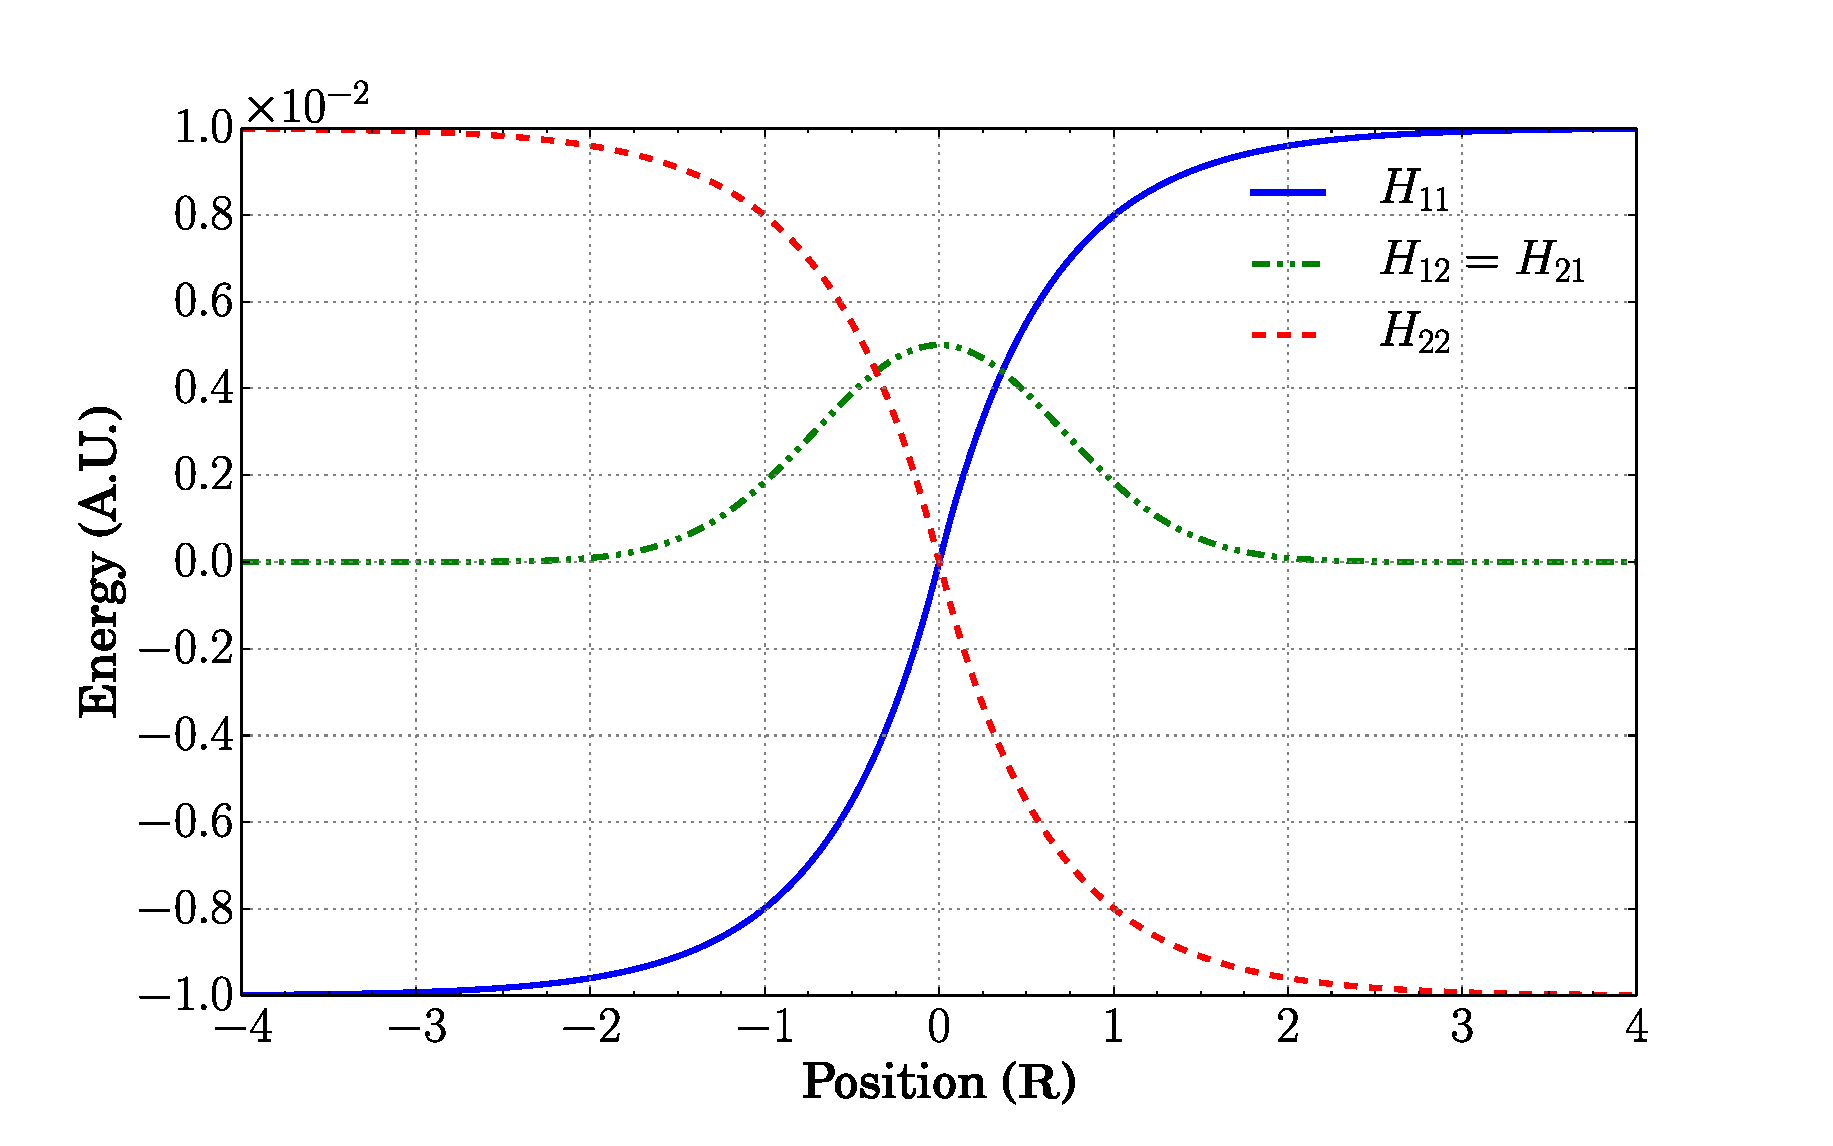
\includegraphics[width=\textwidth]{scpes.eps}
\vspace{-0.2cm}
\caption{Diabatic PES.}
\label{f:pessc}
\end{subfigure}
~
\begin{subfigure}[t]{0.45\textwidth}
\centering
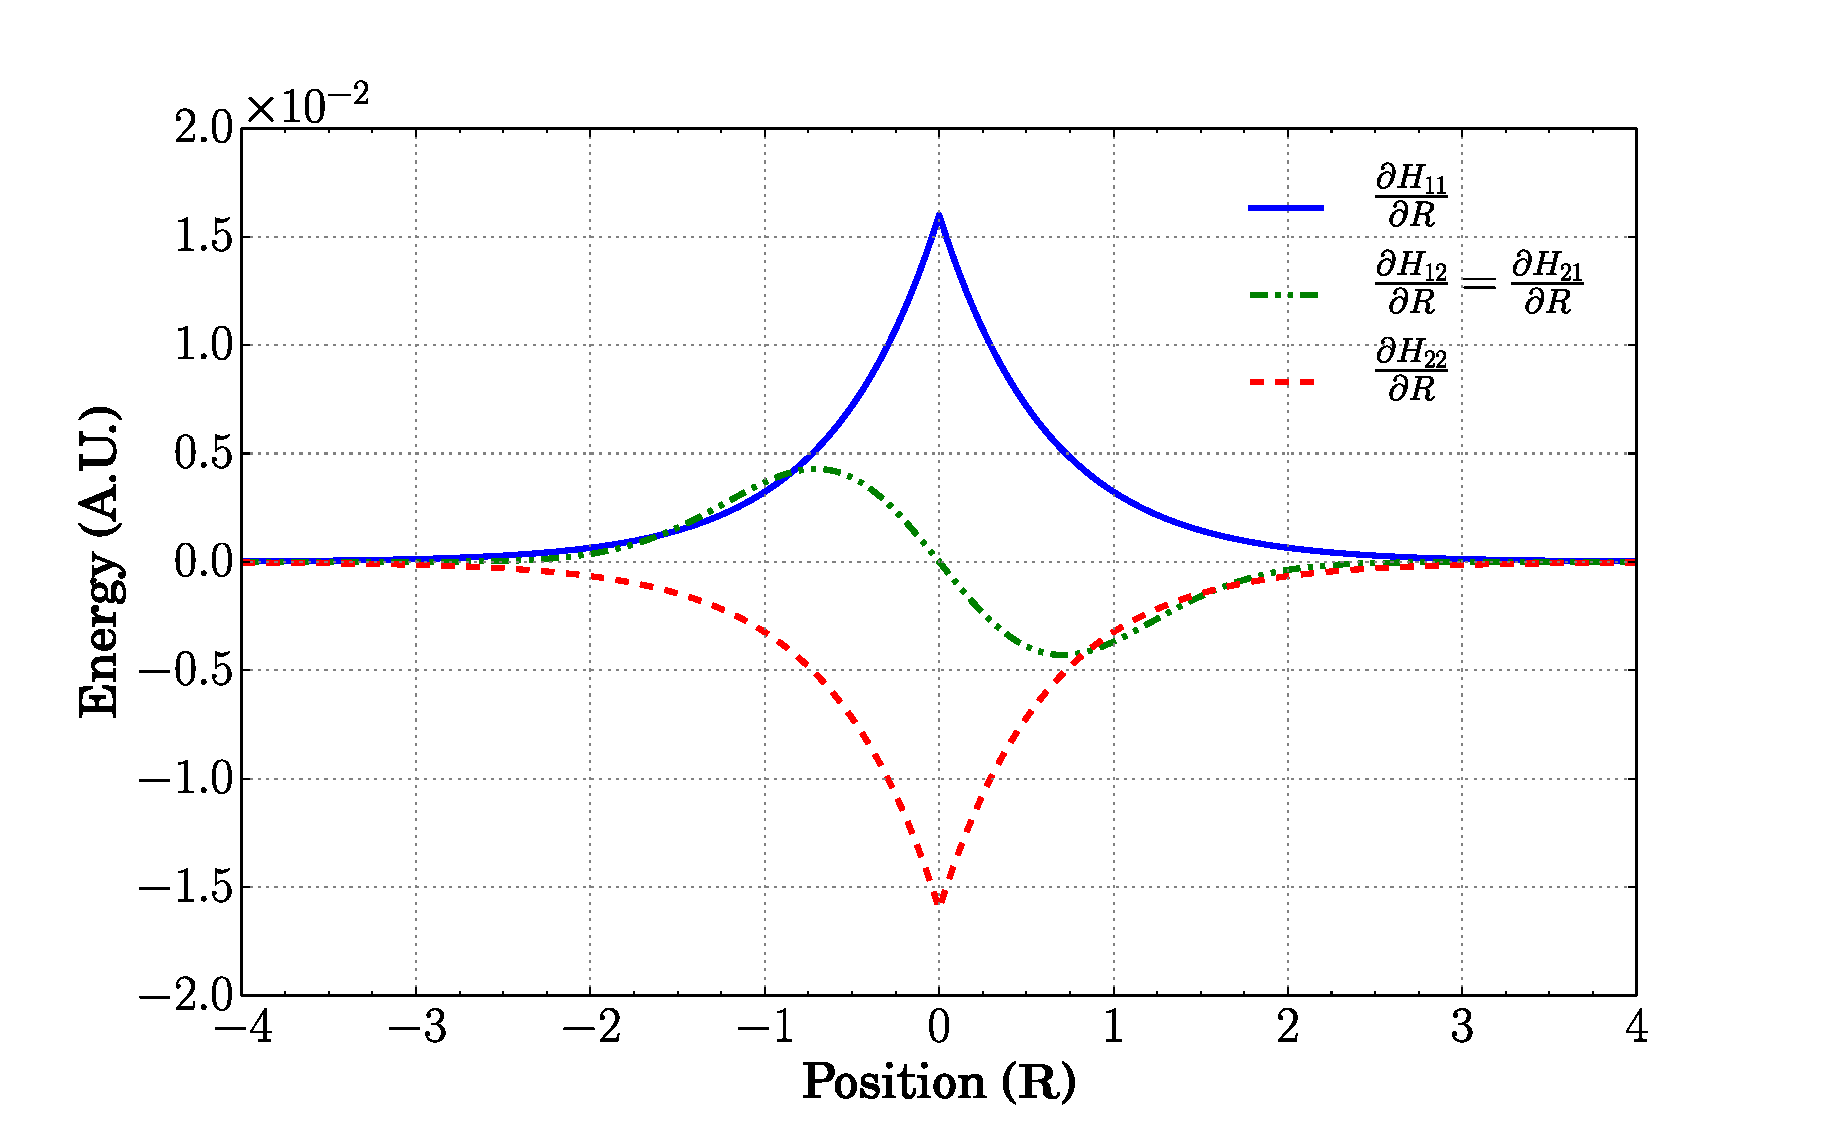
\includegraphics[width=\textwidth]{dscpes.eps}
\vspace{-0.2cm}
\caption{Diabatic PES derivatives (DPES).}
\label{f:dpessc}
\end{subfigure}
\\[-0.35cm]
\begin{subfigure}[t]{0.45\textwidth}
\centering
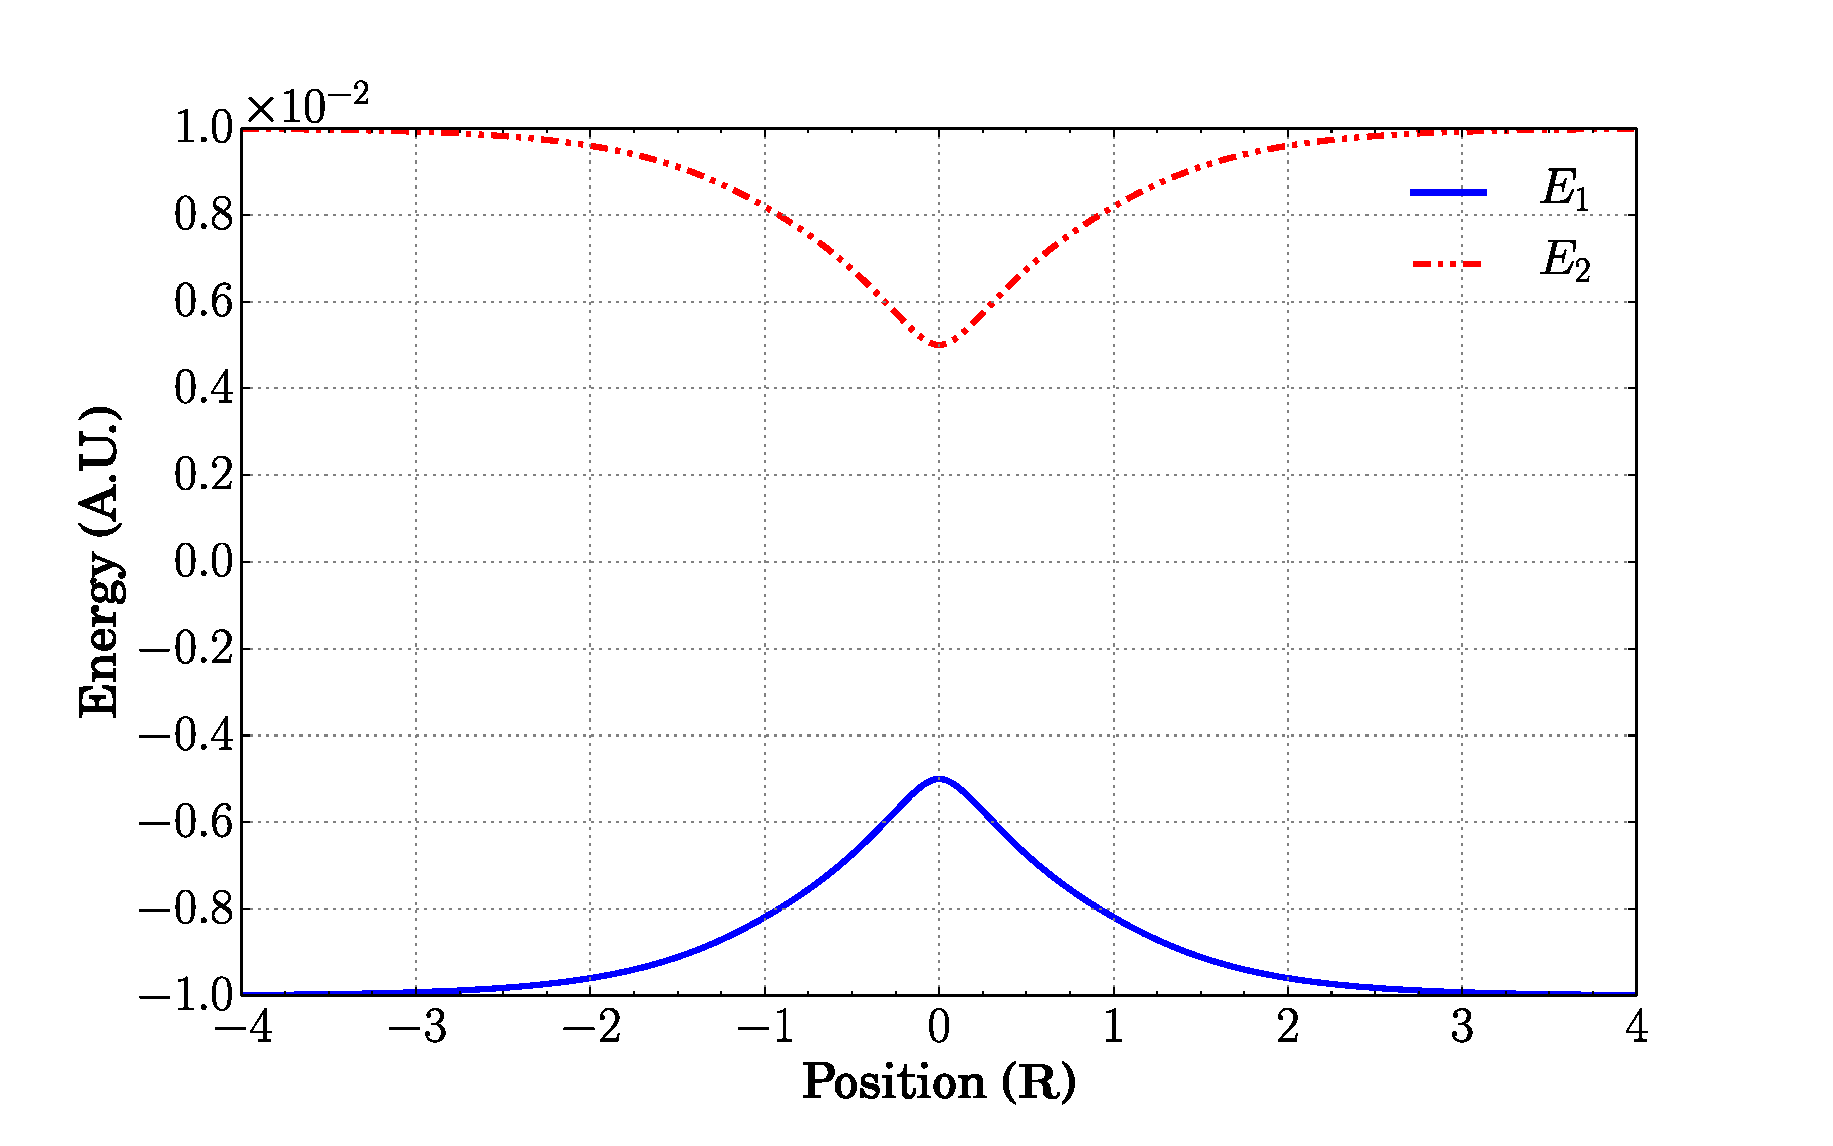
\includegraphics[width=\textwidth]{ascpes.eps}
\vspace{-0.2cm}
\caption{Adiabatic PES (APES).}
\label{f:apessc}
\end{subfigure}
~
\begin{subfigure}[t]{0.45\textwidth}
\centering
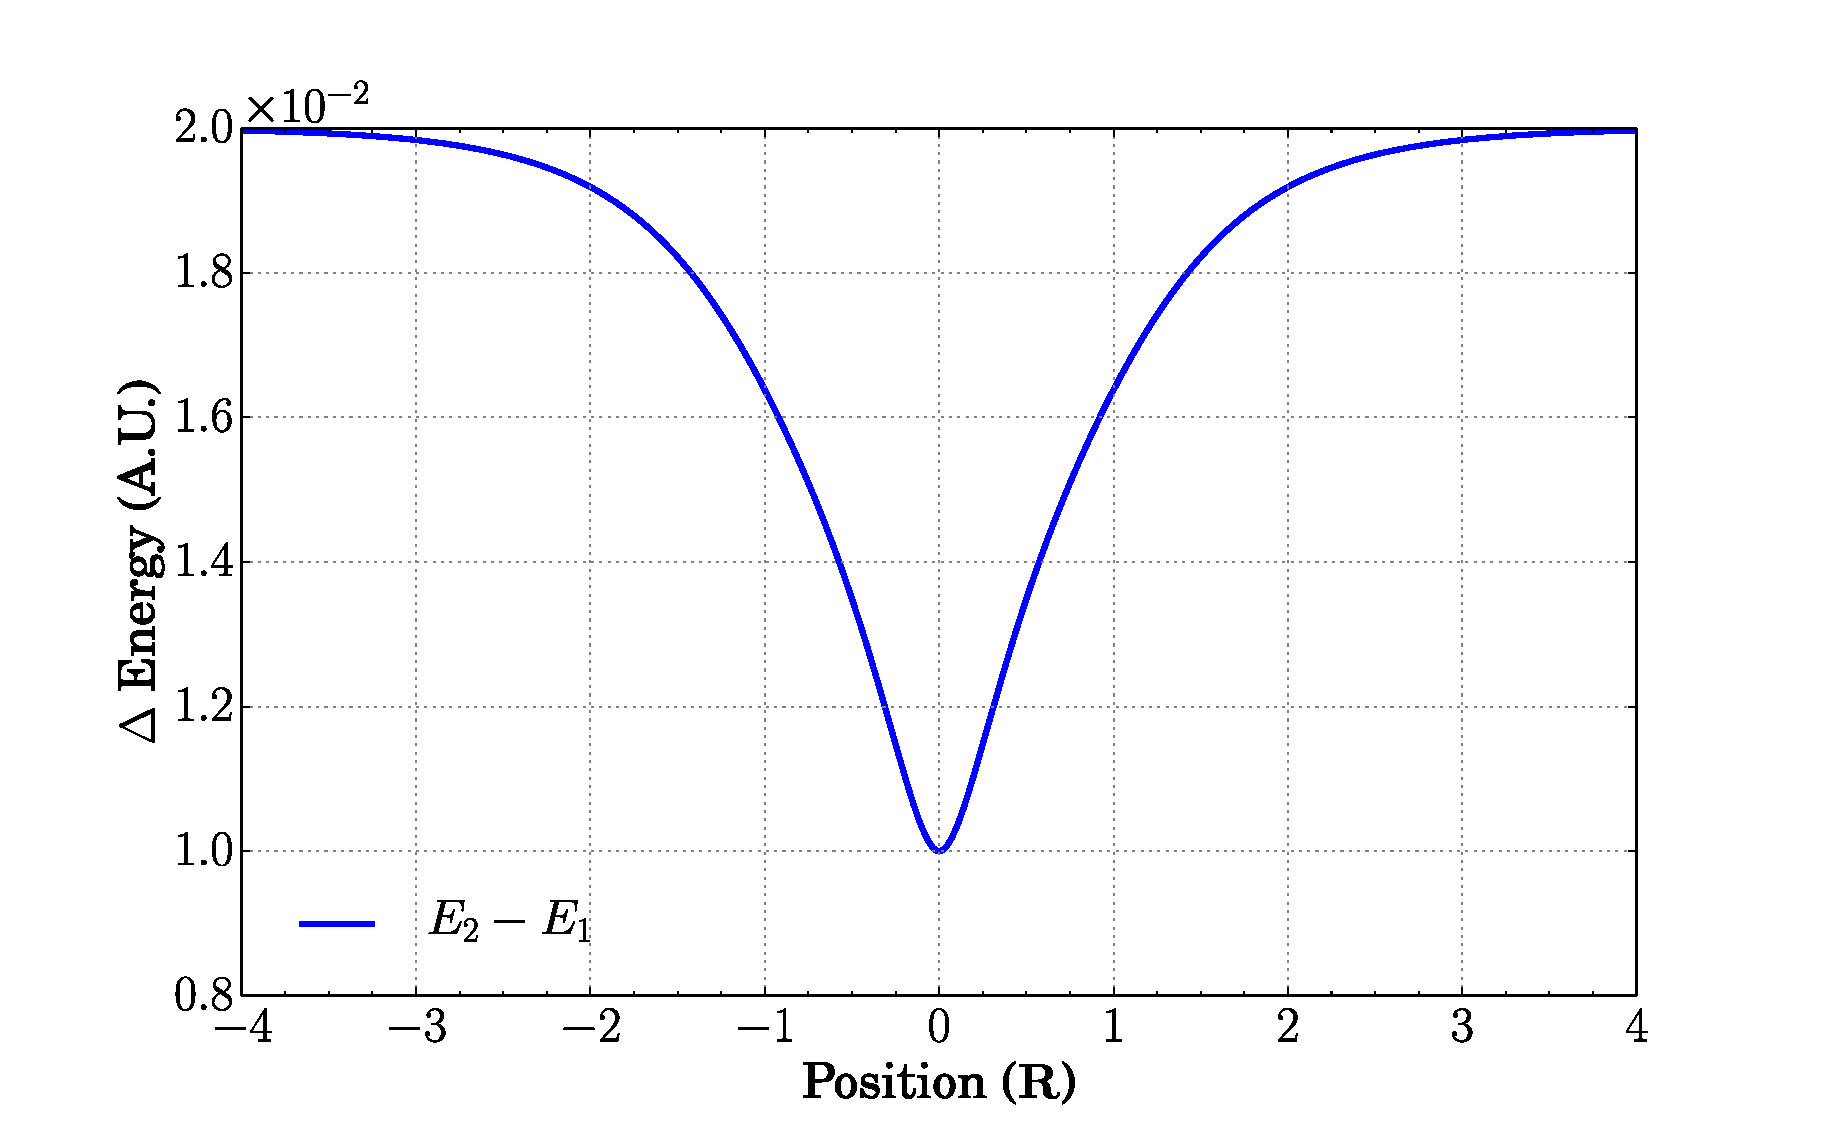
\includegraphics[width=\textwidth]{del_ascpes.eps}
\vspace{-0.2cm}
\caption{$ \Delta E$ between APES.}
\label{f:delapessc}
\end{subfigure}
\vspace{-0.35cm}
\caption{PES.}
\end{figure}
}
\end{frame}

\subsection{Double Avoided Crossing}
\begin{frame}
\frametitle{Double Avoided Crossing}
\alt<1>{
\framesubtitle{Diabatic PES}
\begin{itemize}
\item The diabatic PES were defined by Tully \textcolor{blue}{\cite{tully}} as:
\end{itemize}
\begin{subequations}
\begin{align}
H_{11}(R) &= 0 \\
H_{22}(R) &= -A e^{-B R^{2}} + E_{0}\\
H_{12}(R) &= H_{21}(R) = C e^{-D R^{2}}
\end{align}
\end{subequations}
\begin{itemize}
\item Where $ A = 0.1$, $B = 0.28$, $C = 0.015$, $D = 0.06$, $E_{0} = 0.05$.
\end{itemize}
}{\stepcounter{equation}}

\only<2>{
\framesubtitle{PES Plots}
\begin{figure}
\vspace{-0.33cm}
\centering
\begin{subfigure}[t]{0.45\textwidth}
\centering
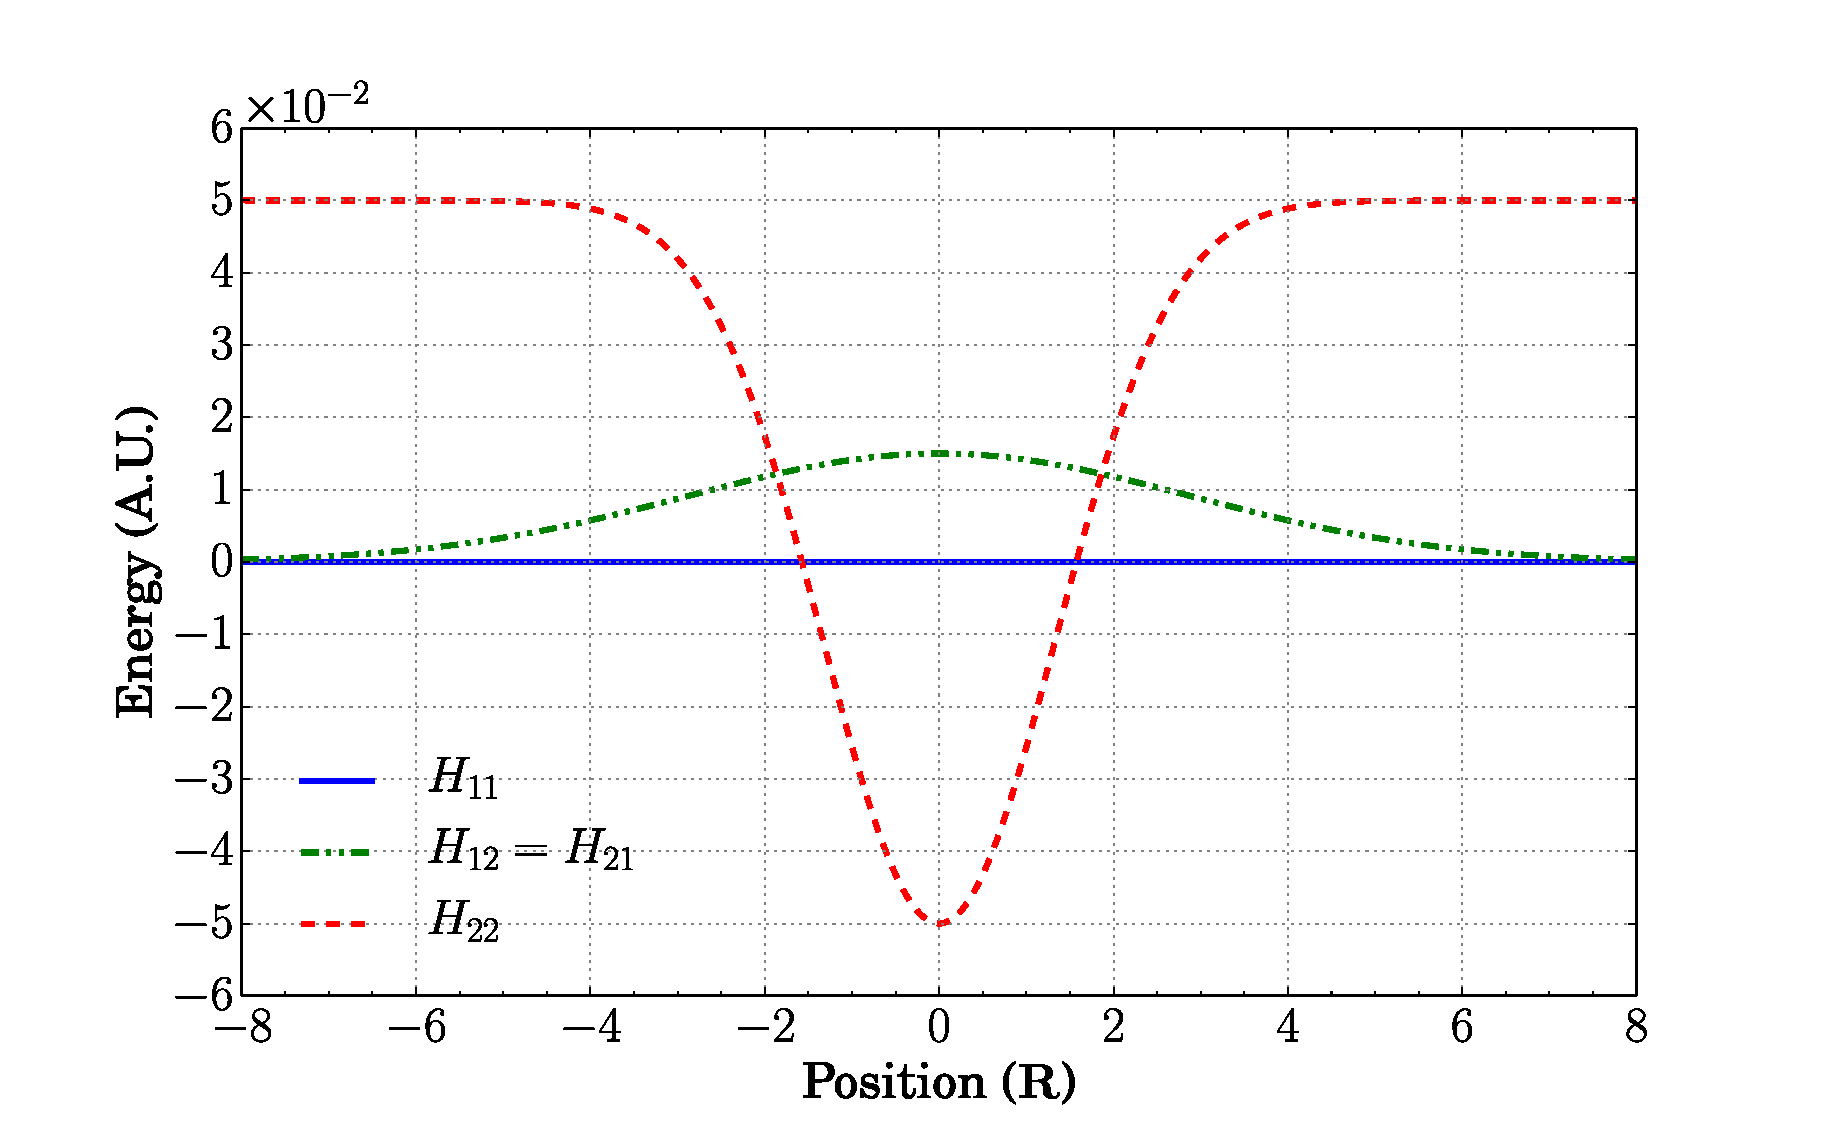
\includegraphics[width=\textwidth]{dcpes.eps}
\vspace{-0.2cm}
\caption{Diabatic PES.}
\label{f:pesdc}
\end{subfigure}
~
\begin{subfigure}[t]{0.45\textwidth}
\centering
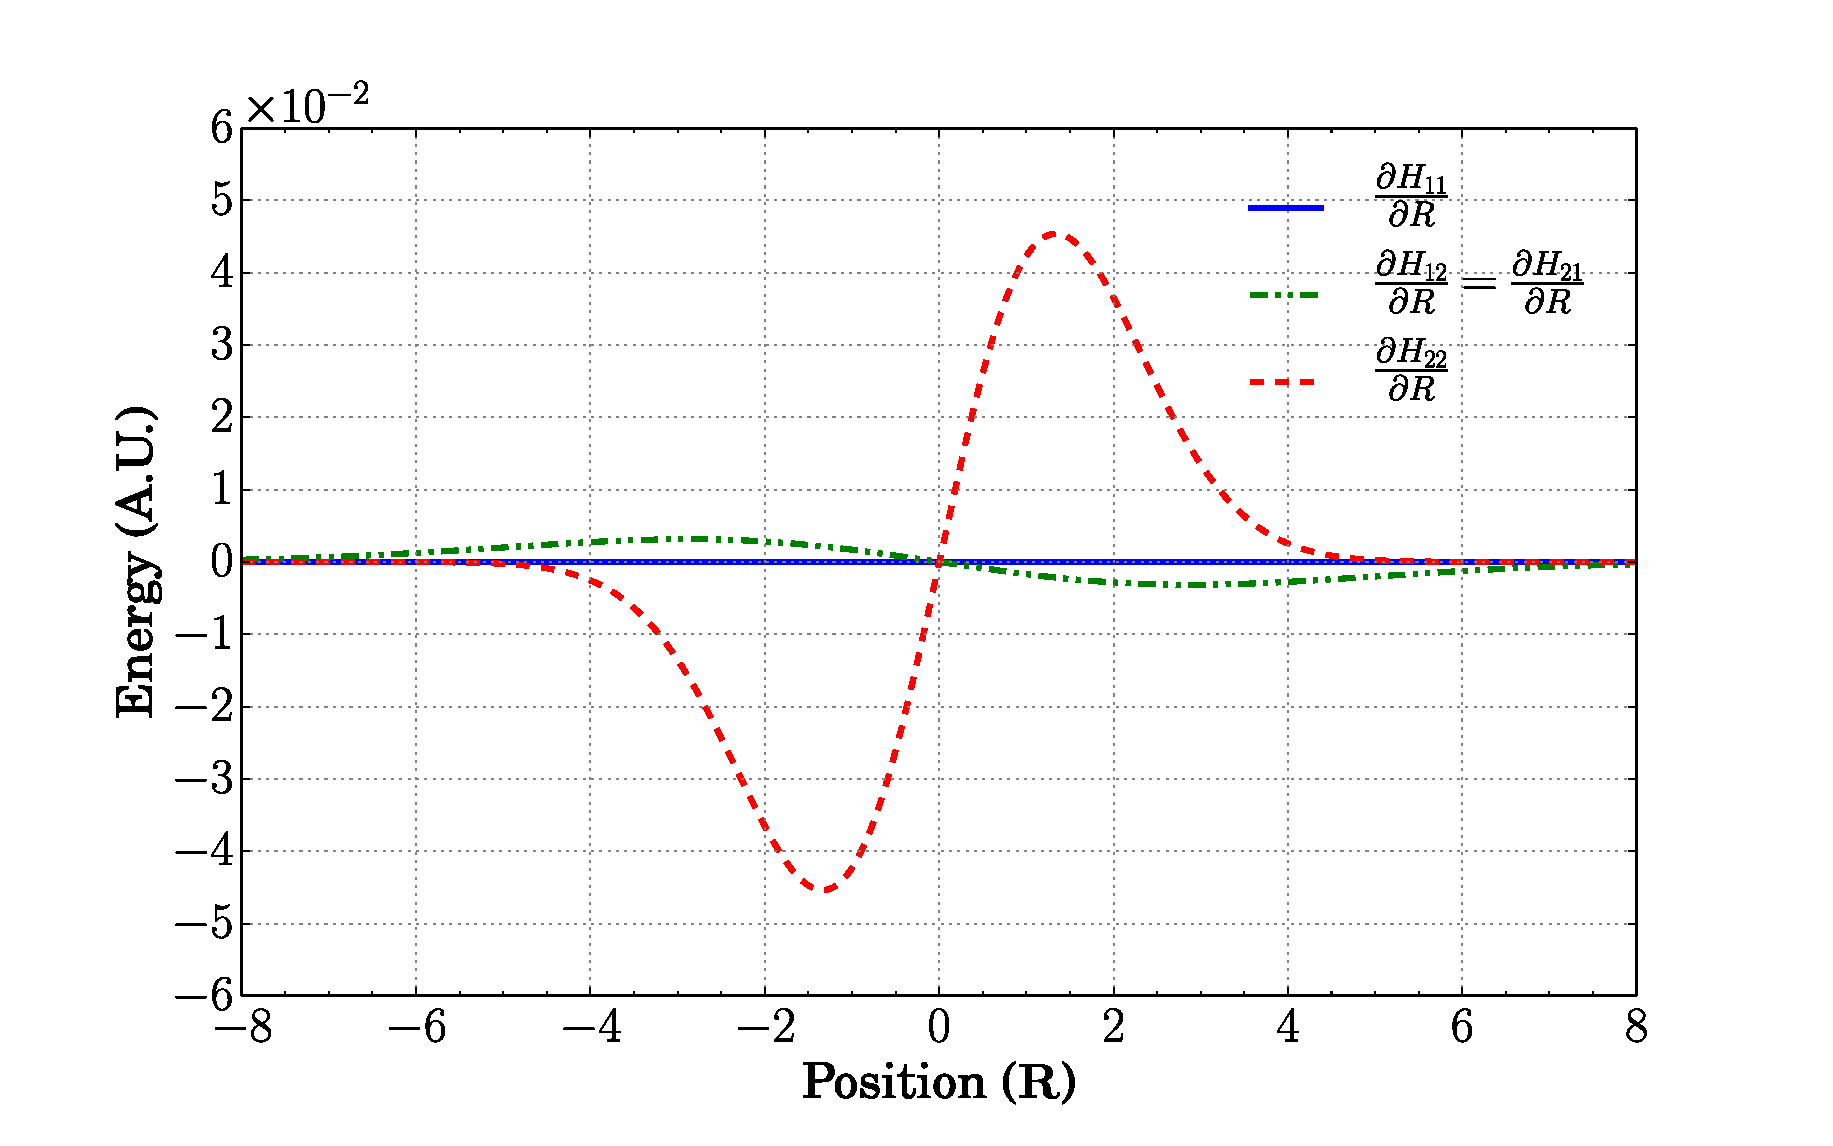
\includegraphics[width=\textwidth]{ddcpes.eps}
\vspace{-0.2cm}
\caption{Diabatic PES derivatives (DPES).}
\label{f:dpesdc}
\end{subfigure}
\\[-0.35cm]
\begin{subfigure}[t]{0.45\textwidth}
\centering
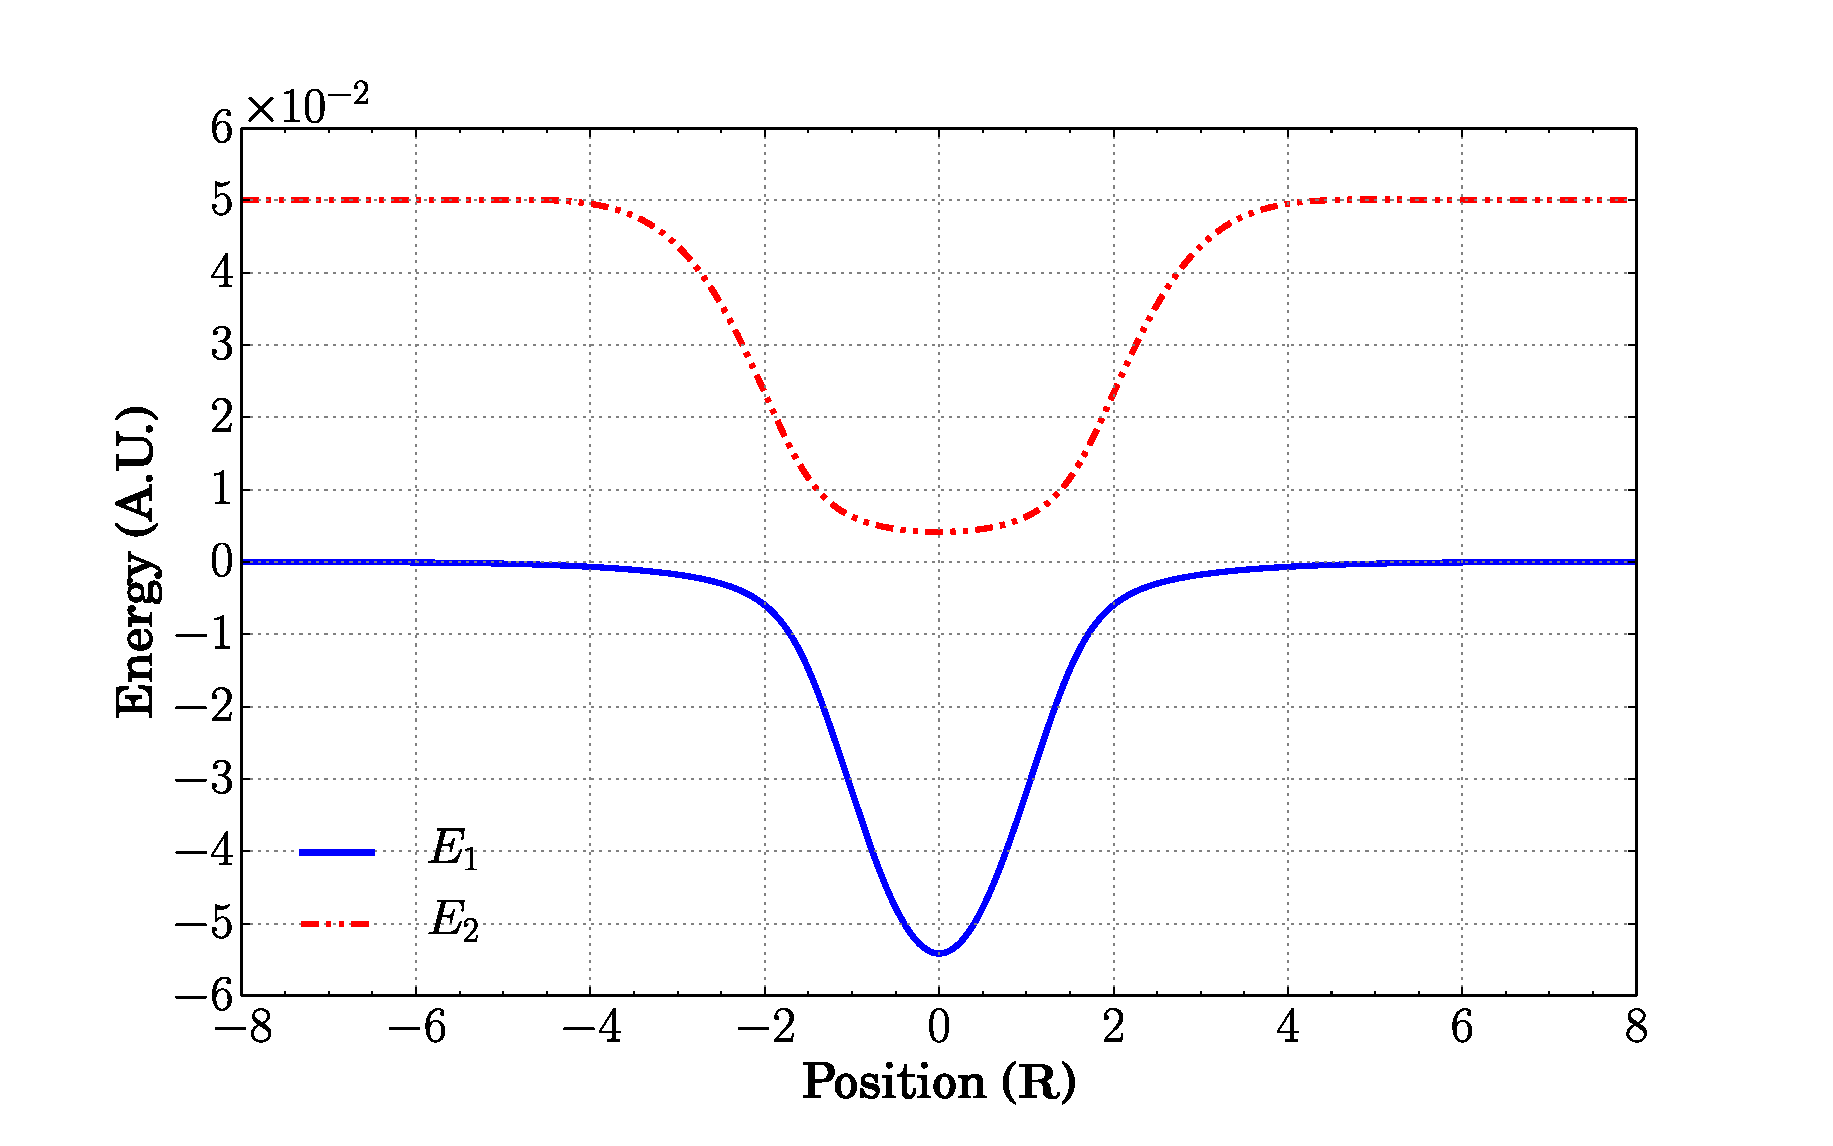
\includegraphics[width=\textwidth]{adcpes.eps}
\vspace{-0.2cm}
\caption{Adiabatic PES (APES).}
\label{f:apesdc}
\end{subfigure}
~
\begin{subfigure}[t]{0.45\textwidth}
\centering
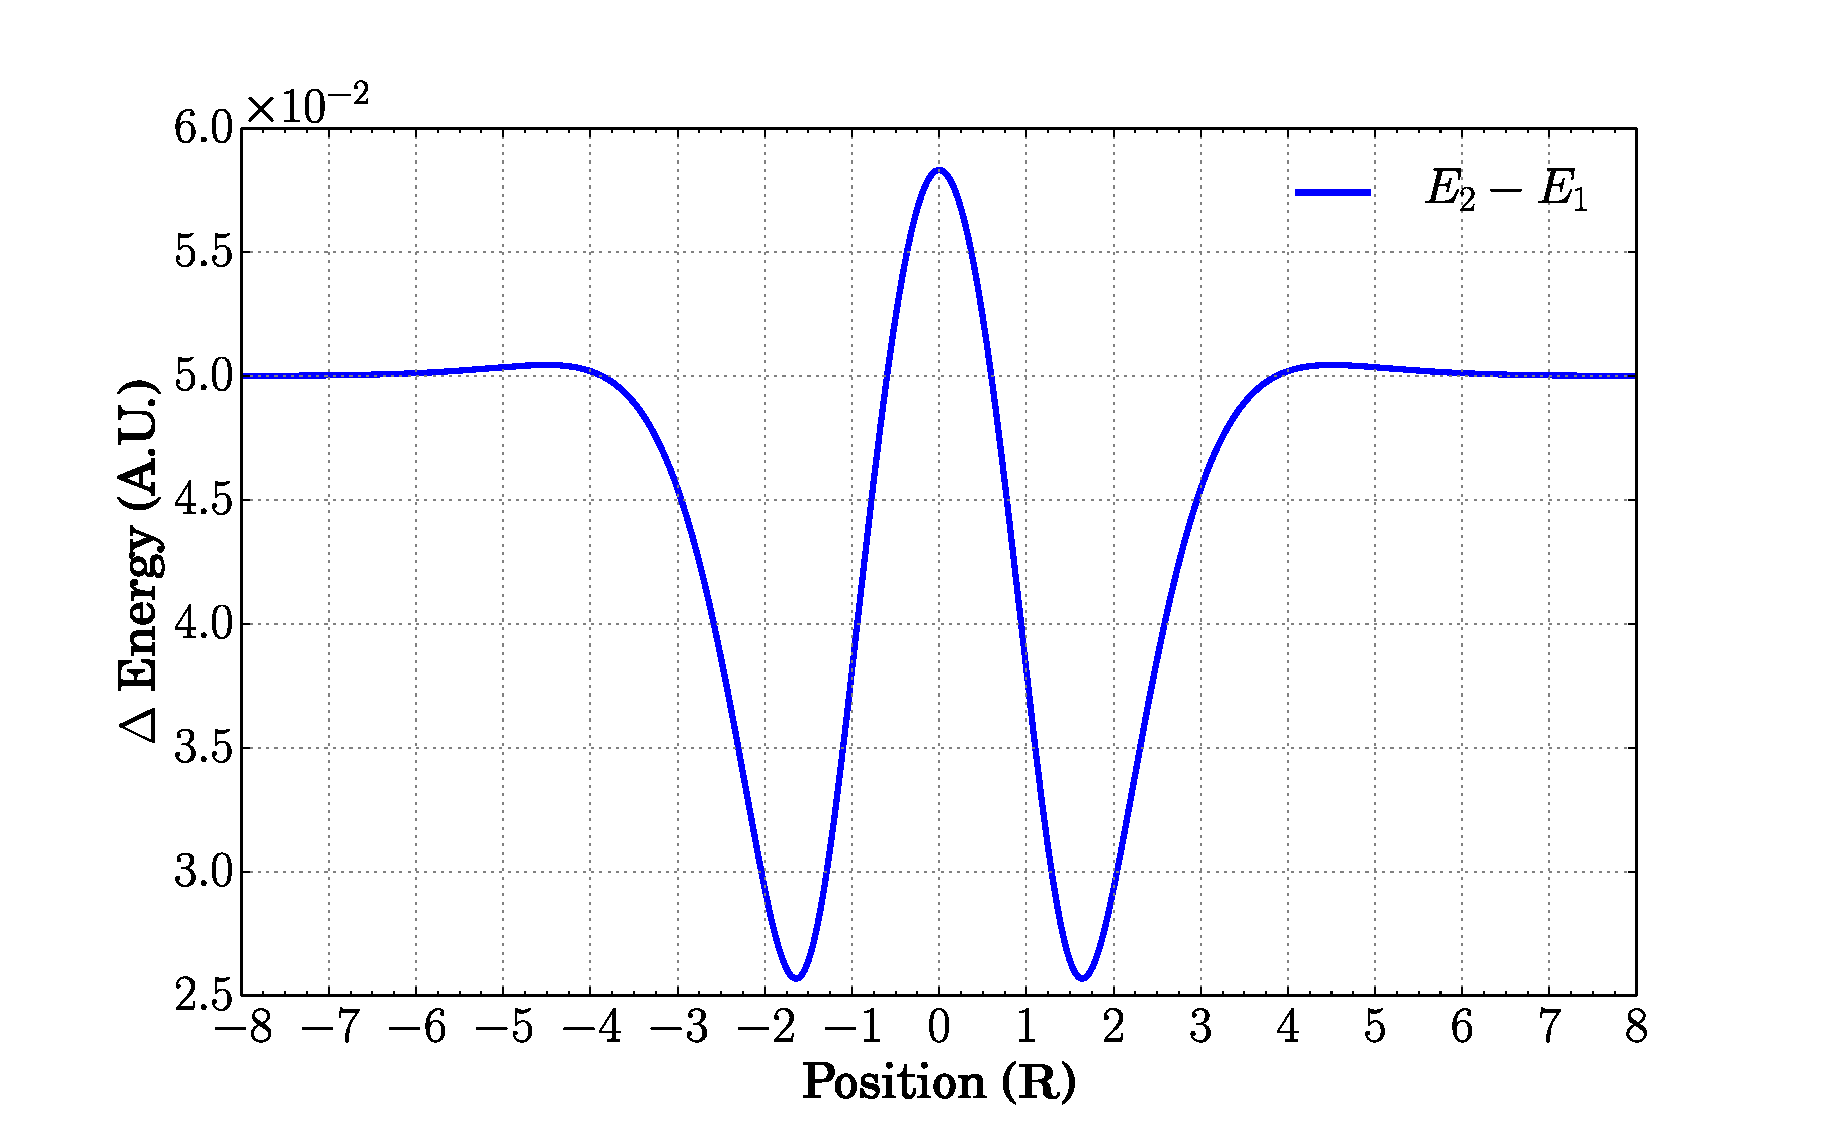
\includegraphics[width=\textwidth]{del_adcpes.eps}
\vspace{-0.2cm}
\caption{$ \Delta E$ between APES.}
\label{f:delapesdc}
\end{subfigure}
\vspace{-0.35cm}
\caption{PES.}
\end{figure}
}
\end{frame}

\subsection{Extended Coupling}
\begin{frame}
\frametitle{Extended Coupling}
\alt<1>{
\begin{itemize}
\item In order to use the diabatic Hamiltonian the non-diagonal PES must vanish as $ R \rightarrow \pm \infty $, so we will use the adiabatic version.
\end{itemize}
\framesubtitle{Diabatic PES}
\begin{itemize}
\item The diabatic PES were defined by Tully \textcolor{blue}{\cite{tully}} as:
\end{itemize}
\begin{subequations}
\begin{align}
H_{11}(R) & = -A\\
H_{22}(R) & = -H_{11}\\
H_{12}(R) & = H_{21}(R) = 
\begin{cases}
B(2 - e^{-C R}) &\mbox{if } R\geq 0 \\
B e^{C R} &\mbox{if } R<0
\end{cases}
\end{align}
\end{subequations}
\begin{itemize}
\item Where $ A = 6 \times 10^{-4}$, $B = 0.1$, $C = 0.9$.
\end{itemize}
}{\stepcounter{equation}}

\only<2>{
\framesubtitle{PES Plots}
\begin{figure}
\vspace{-0.33cm}
\centering
\begin{subfigure}[t]{0.45\textwidth}
\centering
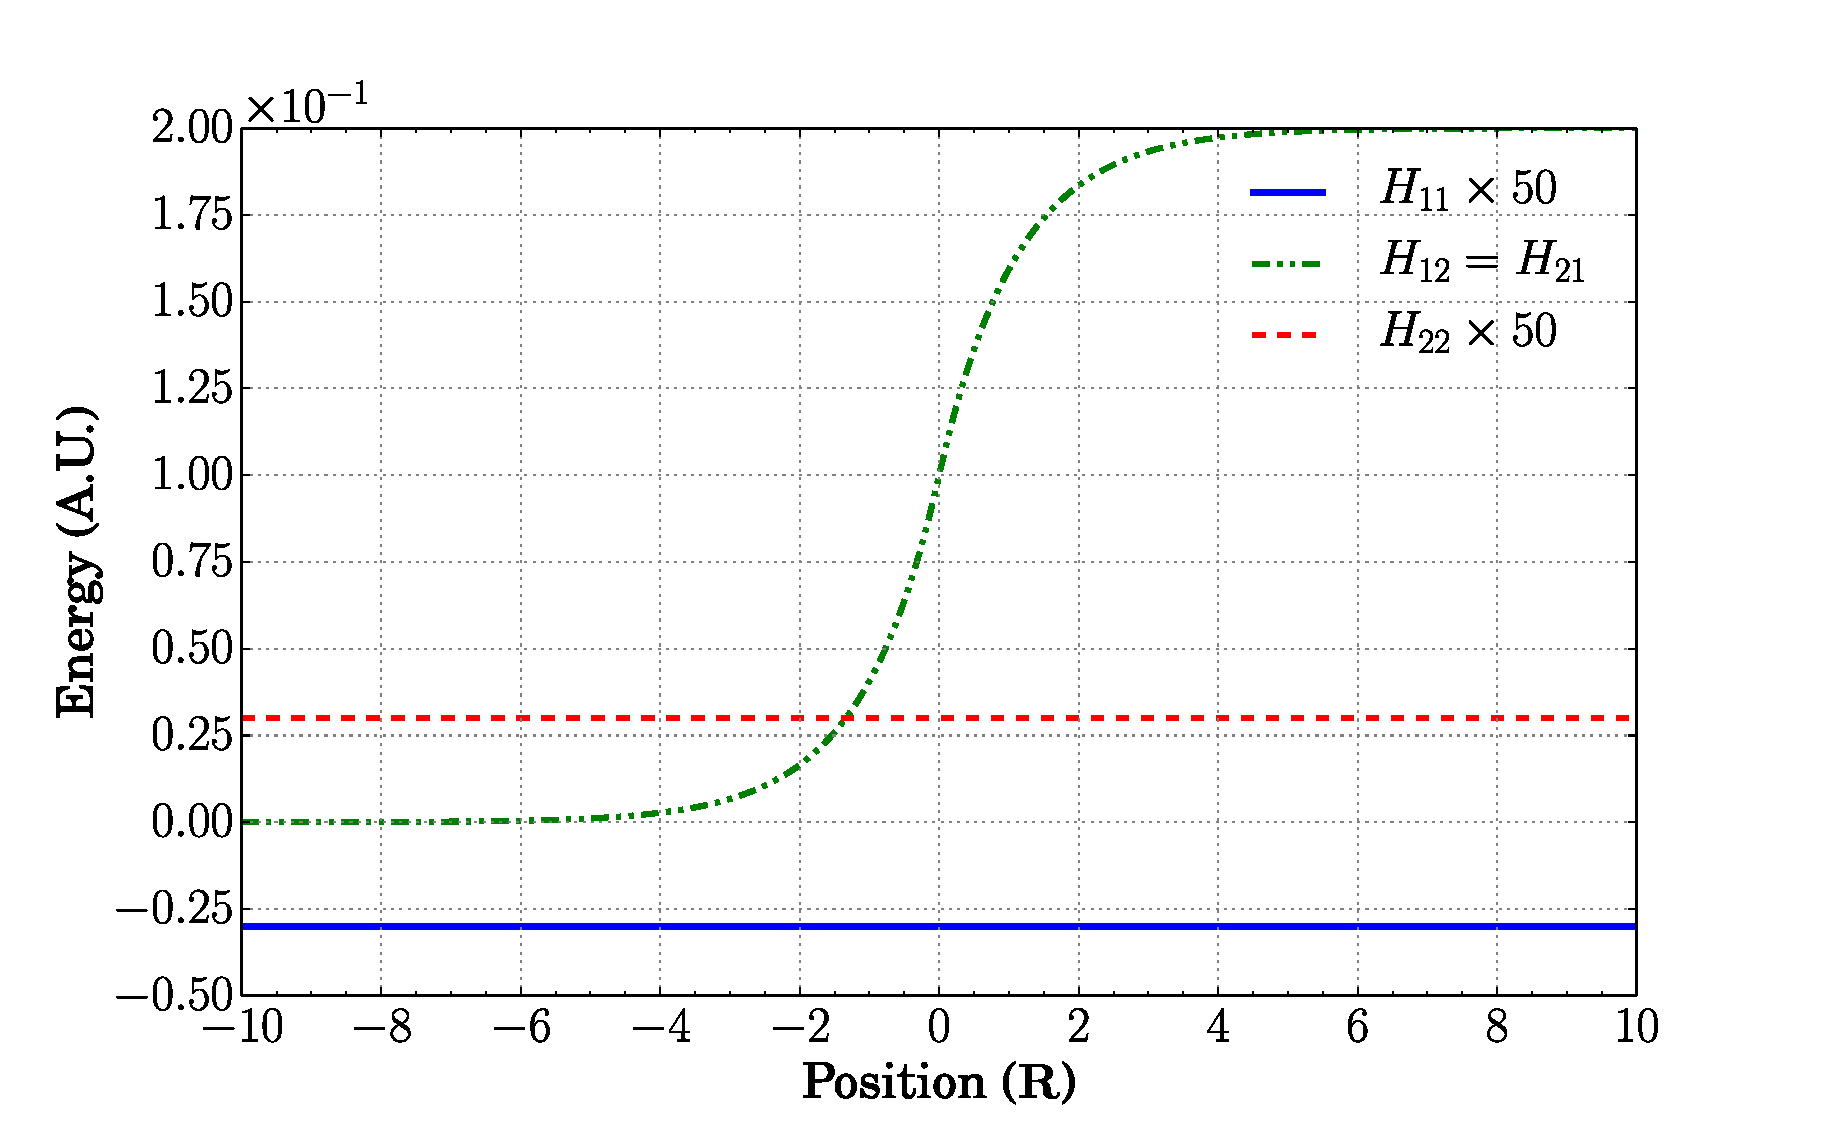
\includegraphics[width=\textwidth]{ecpes.eps}
\vspace{-0.25cm}
\caption{Diabatic PES.}
\label{f:pesec}
\end{subfigure}
~
\begin{subfigure}[t]{0.45\textwidth}
\centering
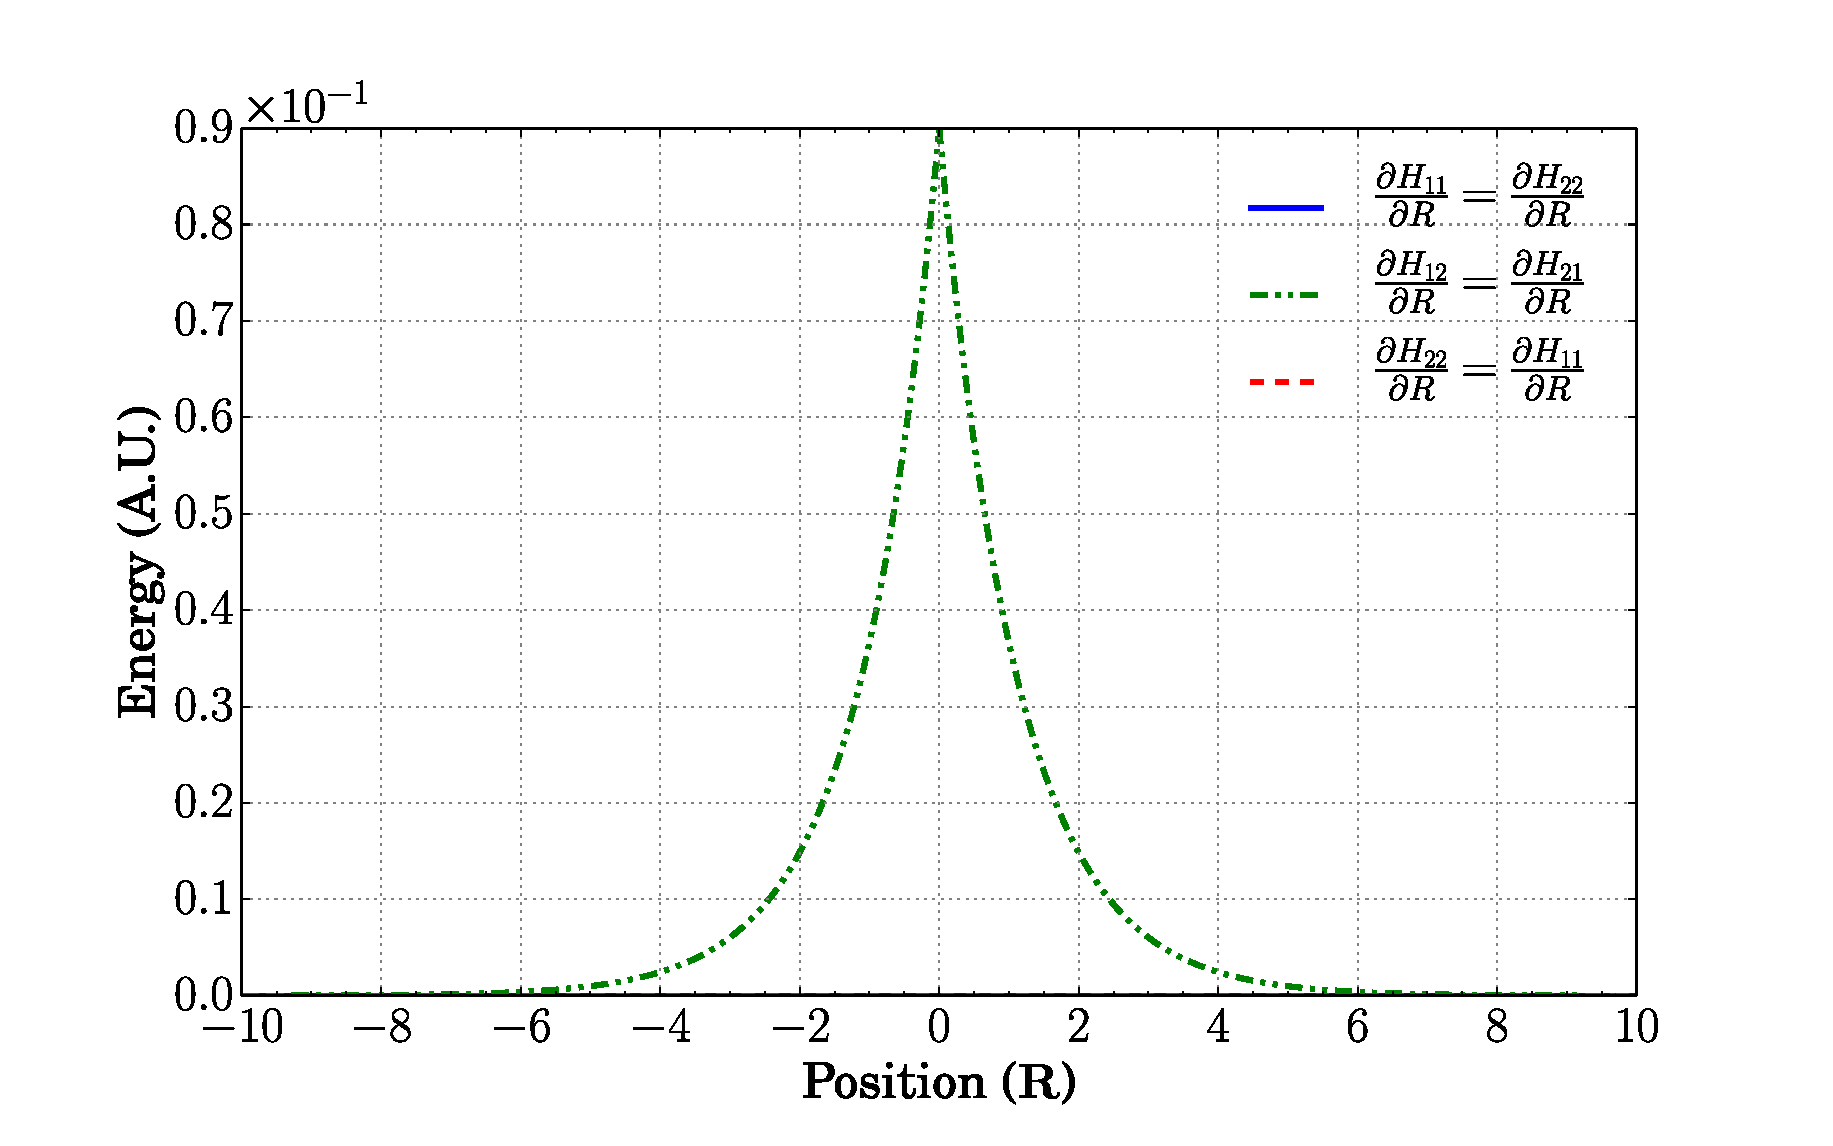
\includegraphics[width=\textwidth]{decpes.eps}
\vspace{-0.25cm}
\caption{Diabatic PES derivatives (DPES).}
\label{f:dpesec}
\end{subfigure}
\\[-0.35cm]
\begin{subfigure}[t]{0.45\textwidth}
\centering
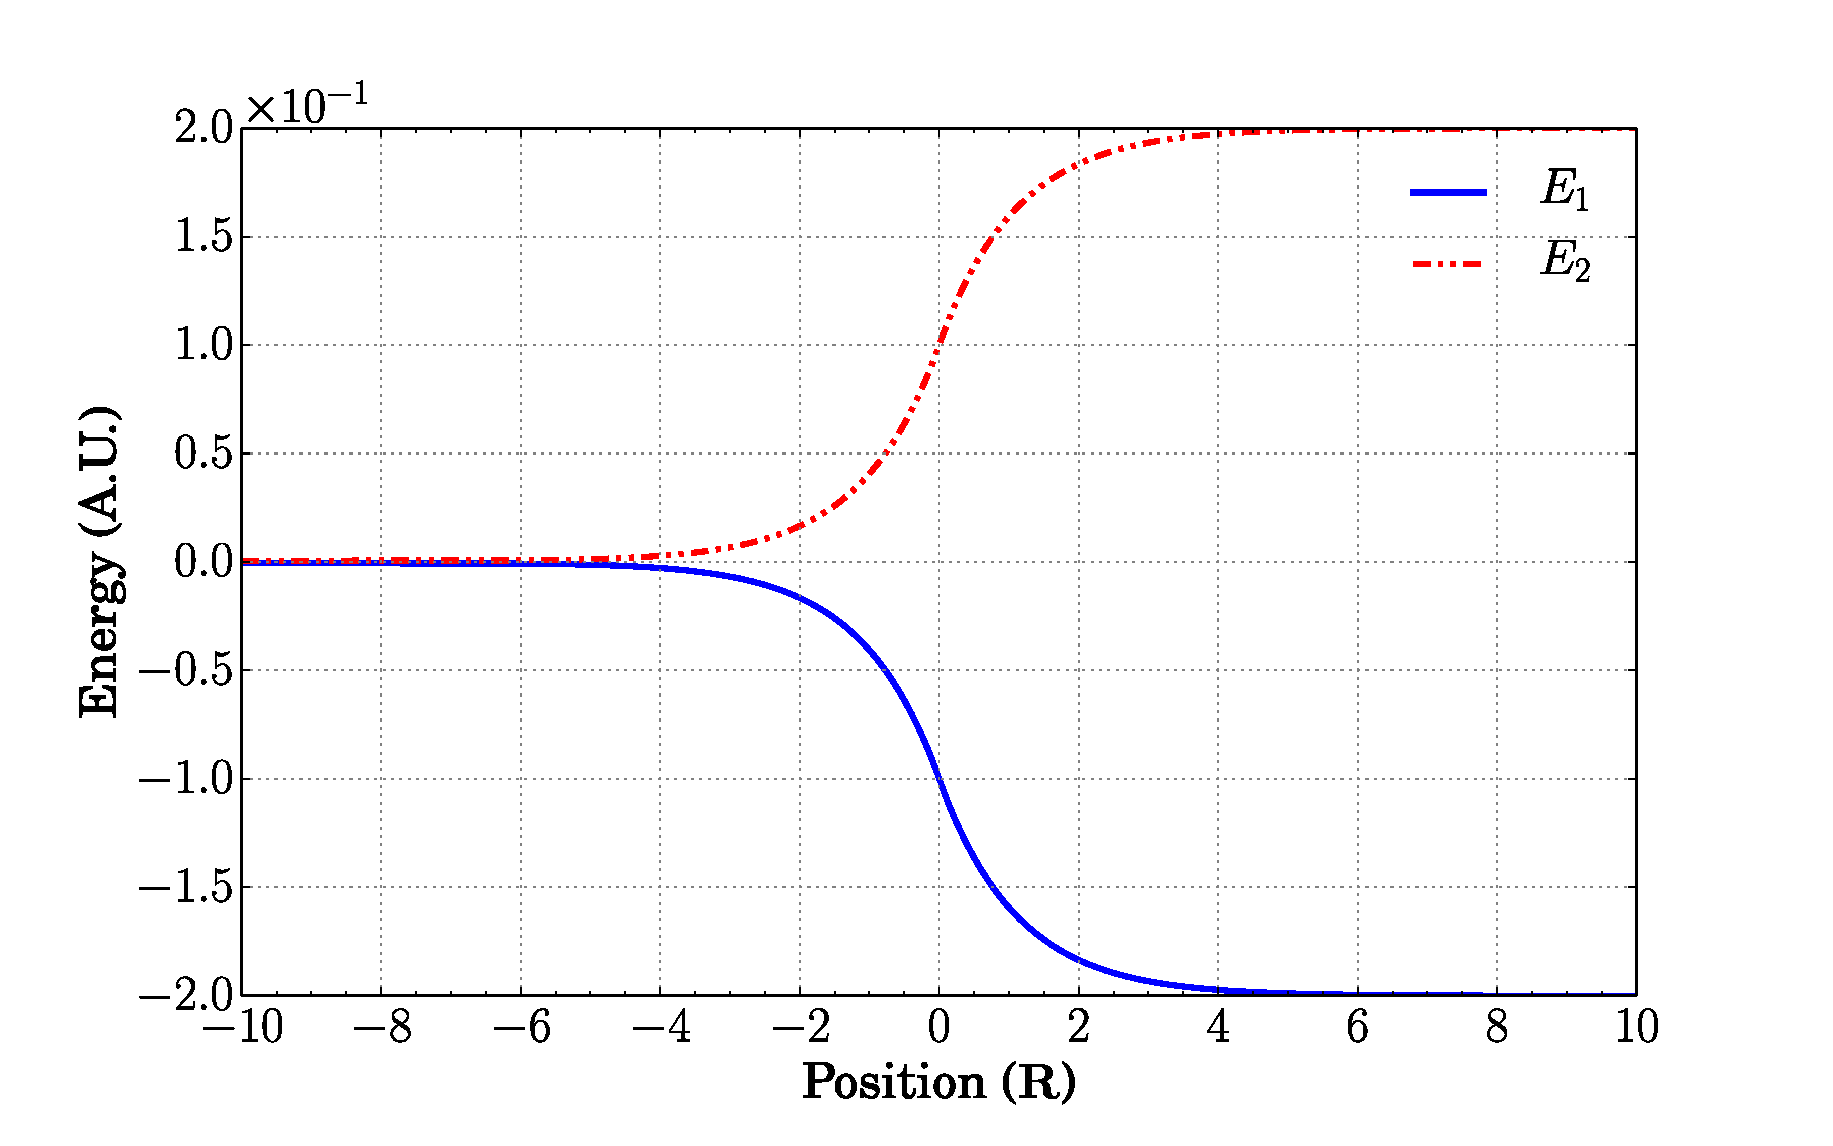
\includegraphics[width=\textwidth]{aecpes.eps}
\vspace{-0.25cm}
\caption{Adiabatic PES (APES).}
\label{f:apesec}
\end{subfigure}
~
\begin{subfigure}[t]{0.45\textwidth}
\centering
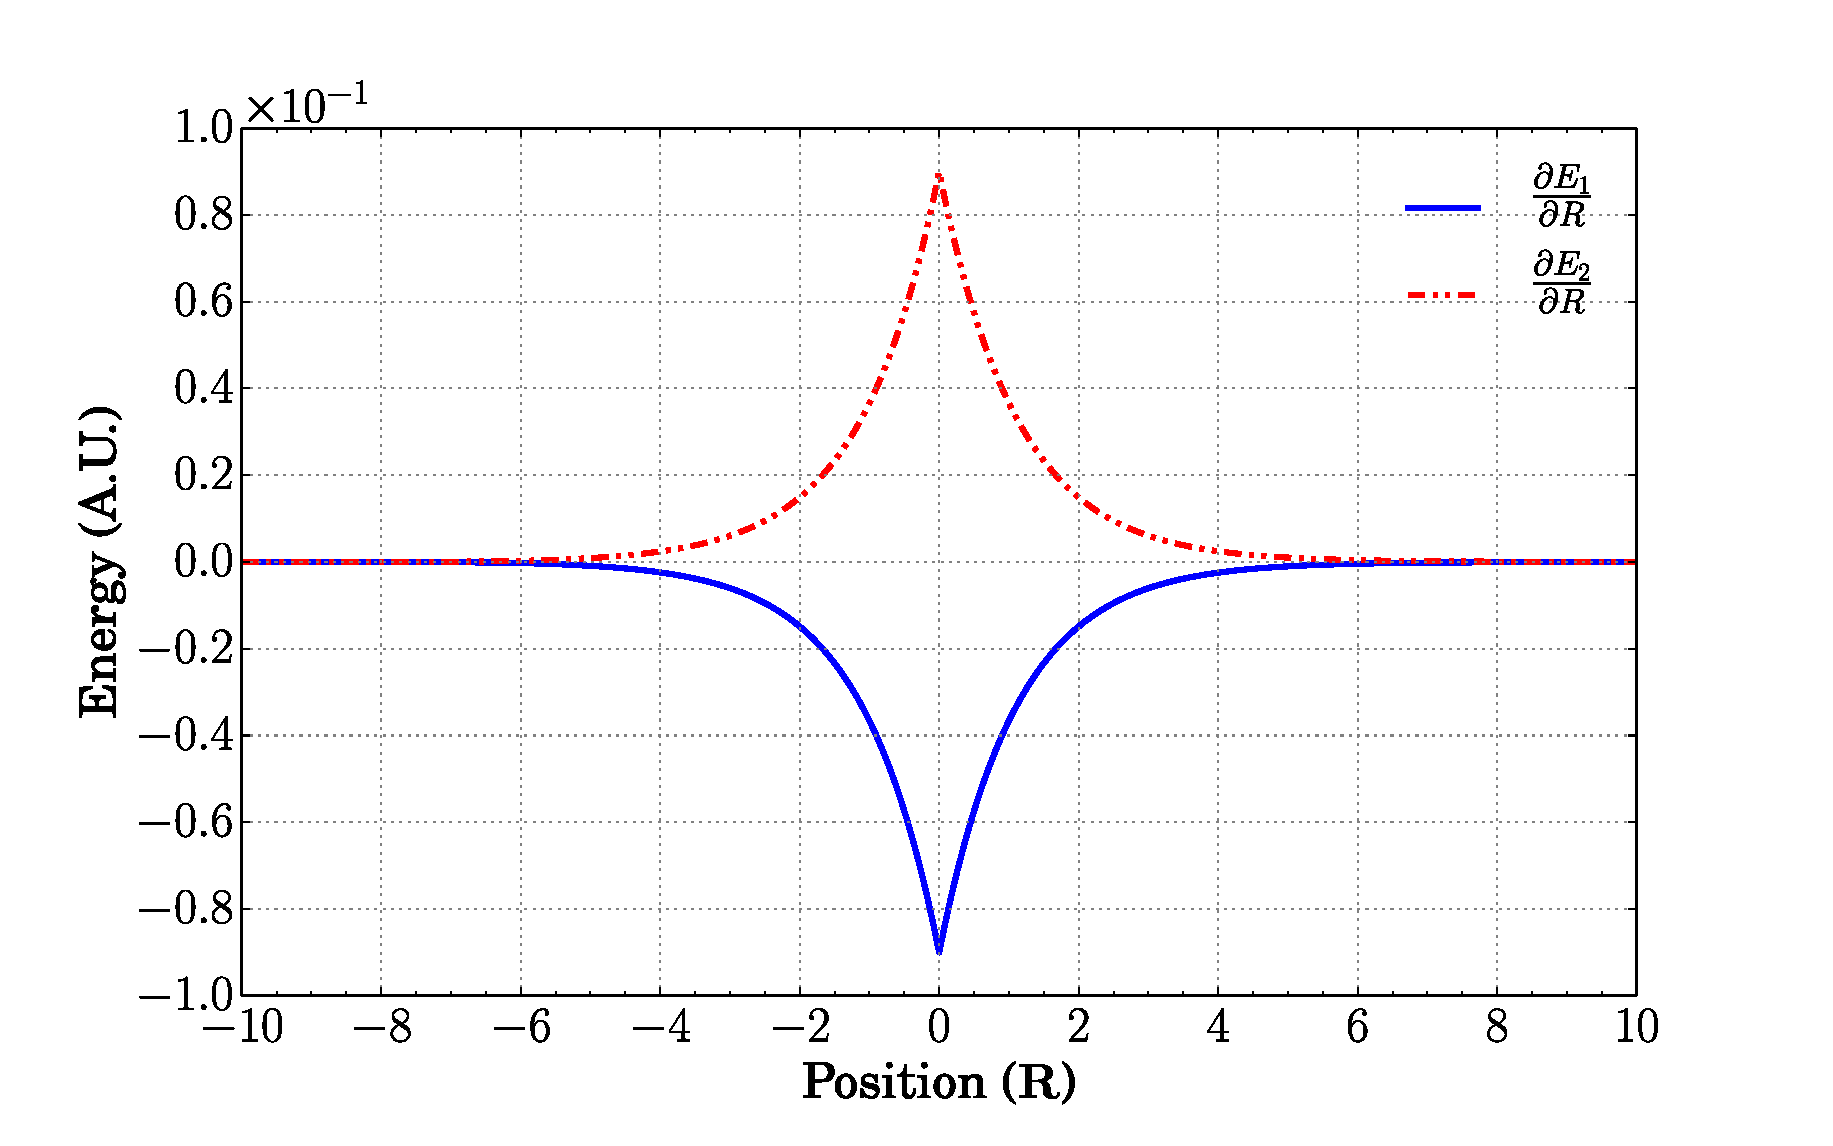
\includegraphics[width=\textwidth]{daecpes.eps}
\vspace{-0.25cm}
\caption{APES derivatives.}
\label{f:dapesec}
\end{subfigure}
\vspace{-0.45cm}
\caption{PES.}
\end{figure}
}
\end{frame}

\subsection{Condensed-Phase Spin-Boson Model}
\begin{frame}
\frametitle{Spin-Boson}
\alt<1>{
\framesubtitle{Generalities}
\begin{itemize}
\item 1D lattice of $ M $ coupled oscillators.
\item Bulk electronic states.
\item The measured quantity is the difference in the probability of both states. When $ i = 1 $, $ D(t) = P_{1\leftarrow 1} - P_{2\leftarrow 1} $; when $ i = 2 $, $ D(t) = P_{1\leftarrow 2} - P_{2\leftarrow 2} $.
\end{itemize}
}{}

\alt<2>{
\framesubtitle{Diabatic PES}
\begin{itemize}
\item The diabatic PES are defined as:
\end{itemize}
\begin{subequations}
\begin{align}\label{e:sbpes}
H_{11}(\bm{Q}) &= V_{0}(\bm{Q}) + V_{1}(\bm{Q}) + \epsilon \\
H_{22}(\bm{Q}) &= V_{0}(\bm{Q}) - V_{1}(\bm{Q}) - \epsilon \\
H_{12}(\bm{Q}) &= H_{12}(\bm{Q}) = \Delta \\
V_{0}(\bm{Q}) &= \sum\limits_{k=1}^{M} \frac{1}{2} m_{k} \omega_{k}^{2} Q_{k}^{2} \\
V_{1}(\bm{Q}) &= \sum\limits_{k=1}^{M} c_{k} Q_{k}
\end{align}
\begin{itemize}
\item Where $ \omega \equiv $ oscillation frequency, $ c \equiv $ coupling parameter, $ Q \equiv $ position, $ m \equiv $ mass.
\end{itemize}
\end{subequations}
}{\stepcounter{equation}}

\alt<3>{
\framesubtitle{Frequencies}
\begin{itemize}
\item It was assumed that $ \omega_{k} $ are uniformly distributed $ \in [0.01 \omega_{c},~4 \omega_{c}] $ \textcolor{blue}{\cite{spin-boson}}, where $ \omega_{c} $ is the `characteristic frequency'.
\item Frequencies contribute to the system's energy differently so each has a coupling parameter $ c_{k} $.
\end{itemize}
\begin{subequations}
\begin{align}
c_{k} &= \omega_{k} \sqrt{\alpha \Delta \omega m_{k} \exp\left(-\frac{\omega_{k}}{\omega_{c}}\right)} \\
\Delta \omega &= \frac{\omega_{max} - \omega_{min}}{M - 1}
\end{align}
\begin{itemize}
\item Where $ \alpha \equiv $ Kondo parameter (coupling strength).
\end{itemize}
\end{subequations}
}{\stepcounter{equation}}

\alt<4>{
\framesubtitle{Initial Conditions}
\begin{itemize}
\item Electronic initial conditions are set as before.
\item Nuclear initial conditions are sampled from the bivariate Gaussian distribution:
\end{itemize}
\begin{subequations}
\begin{align}
\rho(\bm{P},\bm{Q}) &= \prod\limits_{k=1}^{M} \exp\left(-a_{k} \frac{P_{k}^{2}}{2 m_{k}}\right)\cdot \exp\left(-a_{k} \frac{1}{2} m_{k} \omega_{k}^{2} \left[Q_{k} + \frac{c_{k}}{m_{k} \omega_{k}^{2}}\right]^{2} \right)\\
a_{k} &= \frac{2}{\omega_{k}} \tanh\left(\frac{\beta \omega_{k}}{2}\right)
\end{align}
\end{subequations}
}{\stepcounter{equation}}
\end{frame}

\section{Methodology}
\begin{frame}
\frametitle{Methodology}
\begin{itemize}
\item Obtaining equations of motion.
\item Writing code.
\item Testing code.
\item Running problems.
\item Plotting results.
\end{itemize}
\end{frame}

\section{Results}
\subsection{Notation and Assumptions}
\begin{frame}
\frametitle{Notation and Assumptions}
\begin{itemize}
\item A reflection is denoted as $ R $ and a transmission as $ T $.
\item The initial state is denoted as $ i $ and the final state as $ f $.
\item A transition $ G $ from an initial state $ i $ to a final state $ f $ is denoted as $ G_{f\leftarrow i} $.
\item $ h \equiv $ integration interval, $ P_{i} \equiv $ initial momentum and $ E_{i} \equiv $ mean initial energy.
\item Unless otherwise mentioned: all calculations were carried out with $ 15000 $ Monte-Carlo repetitions (MC reps), $ \gamma = 0.366 $, all masses $ \mu = m_{k} = 2000 $, and all units are in atomic units.
\item For the spin-boson model, it was assumed that the number of nuclei $= 100 $ ($ M=100 $) and $ \omega_{c} = 1 $.
\end{itemize}
\end{frame}

\subsection{Code Characterisation}
\begin{frame}
\only<1>{
\frametitle{Generalities}
\begin{itemize}
\item Scaling is linear with MC reps, value of $ h $ and number of cores.
\item The value of $ h $ does not significantly affect the accuracy up to a threshold value, said threshold depends on the problem.
\end{itemize}
}

\only<2>{
\frametitle{Paralellisation}
    \begin{figure}
    \vspace{-0.3cm}
      \begin{columns}
      	\hspace{-2.5cm}
        \column{.7\linewidth}
        \centering
        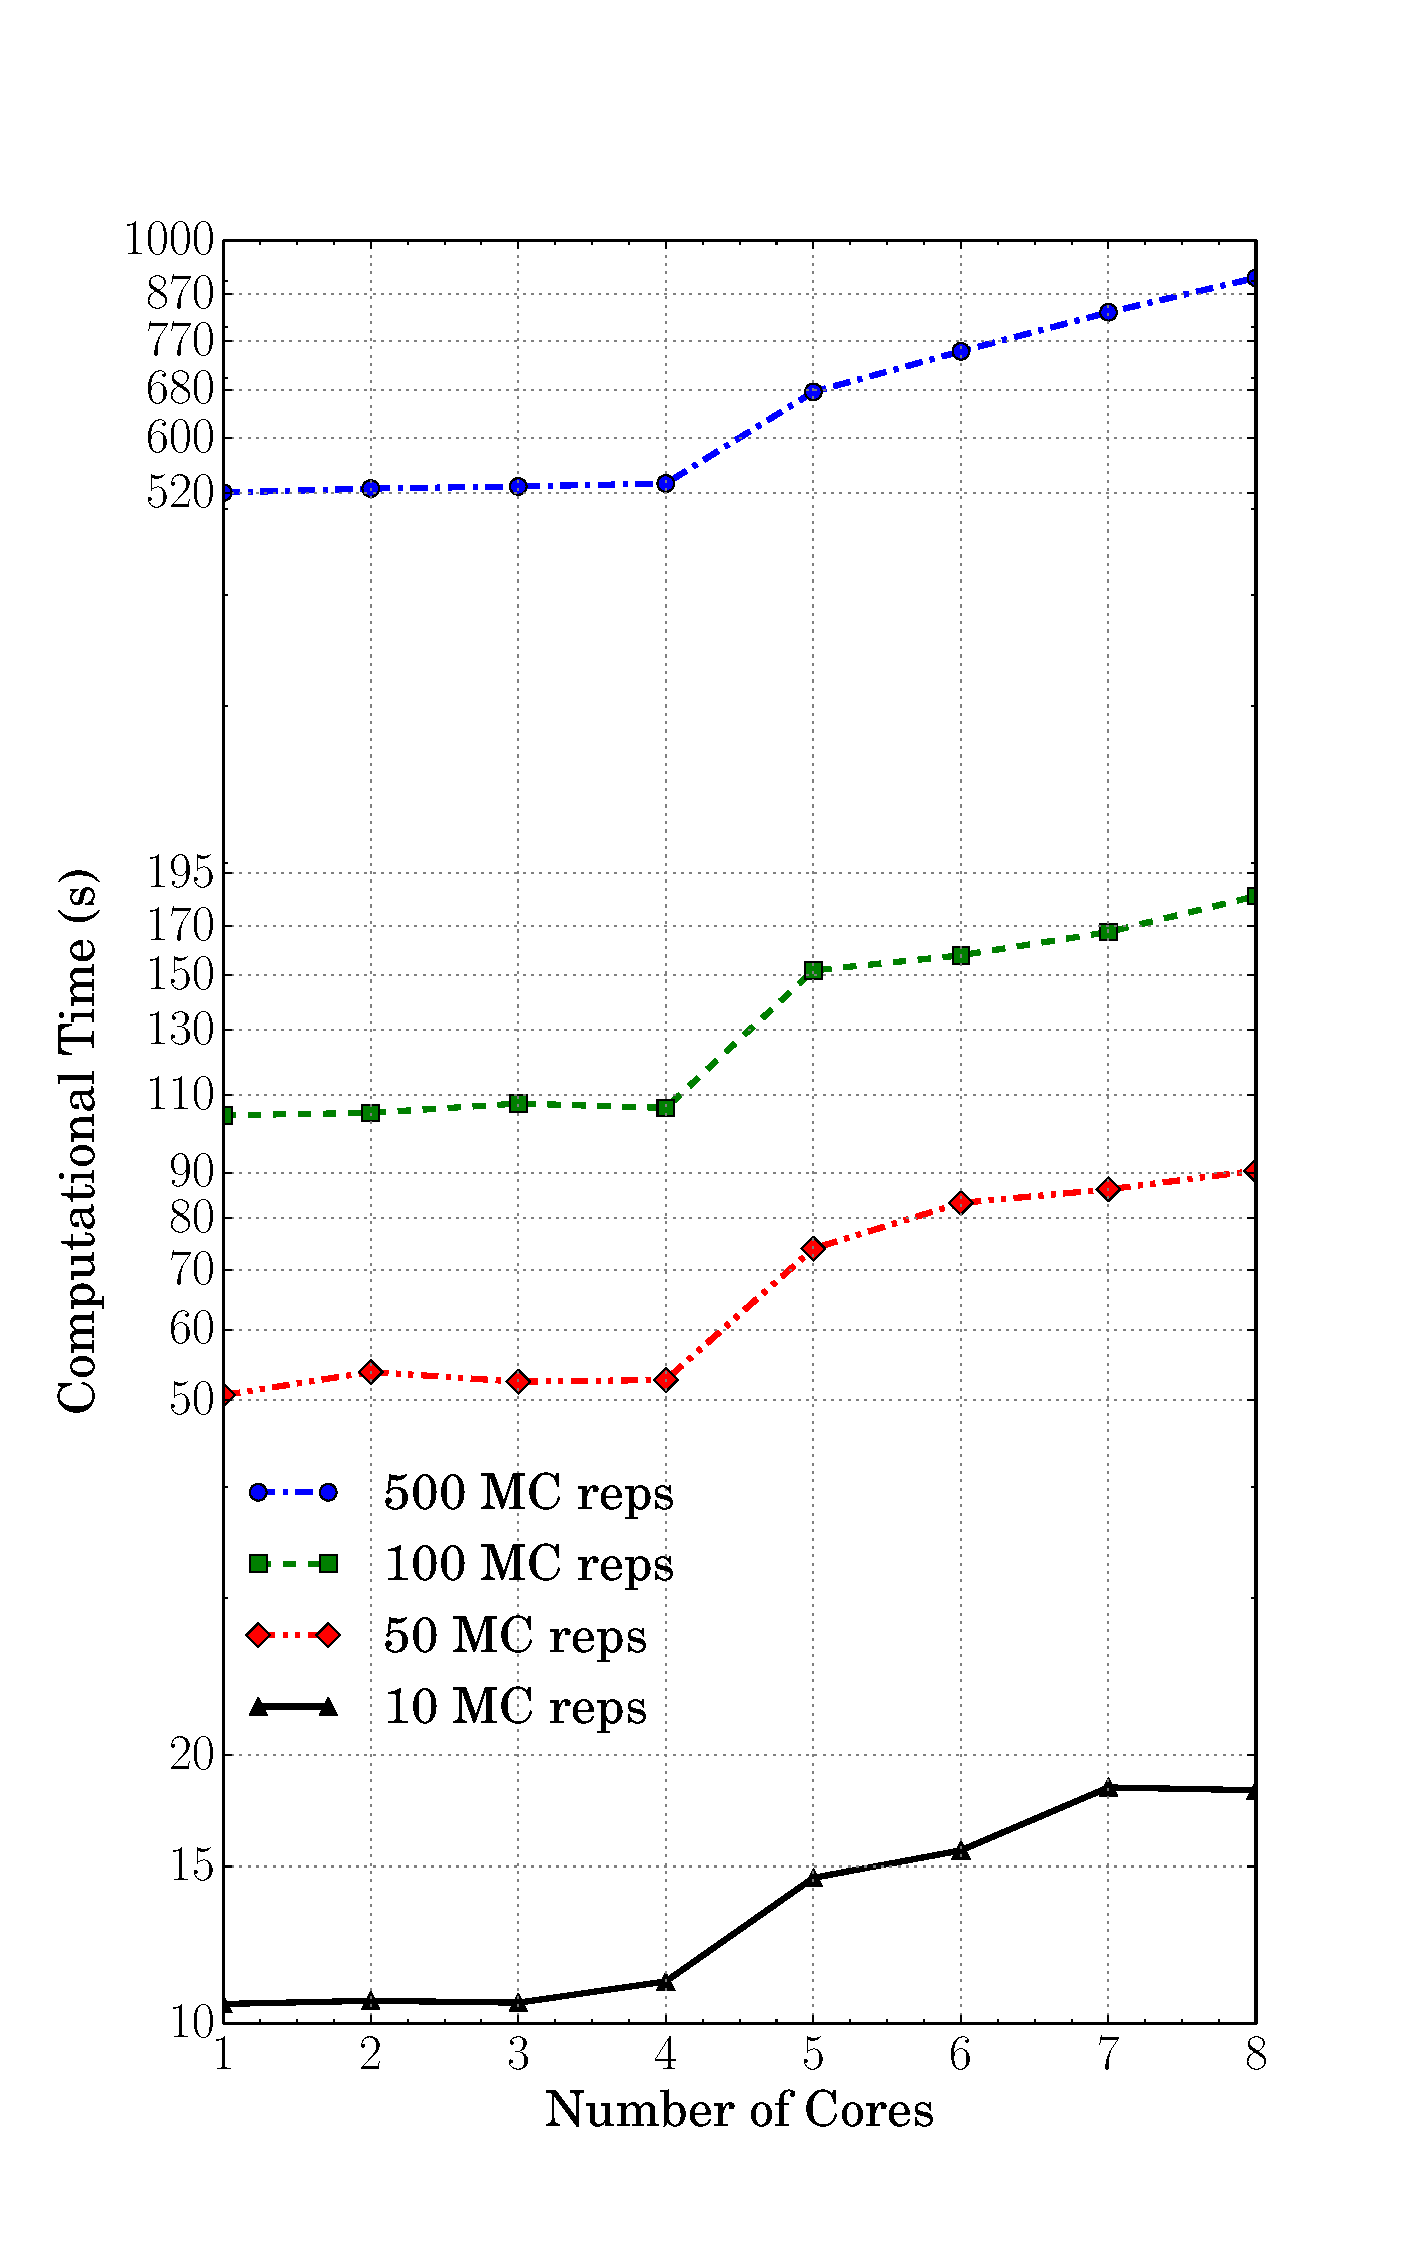
\includegraphics[width=0.68\textwidth]{mpi.eps}
        \hspace{-3cm}
        \column{.5\linewidth}
        \caption{Temporal scaling as a function of nuclei and MC reps. Scaling is directly proportional to the number of MC reps, and inversely proportional to the number of cores.}
        \label{f:mpi}
      \end{columns}
    \end{figure}
}
\end{frame}

\subsection{Single Avoided Crossing}
\begin{frame}
\frametitle{Single Avoided Crossing}
\alt<1>{
\vspace{-0.33cm}
\begin{figure}
\centering
\begin{subfigure}[t]{0.45\textwidth}
\centering
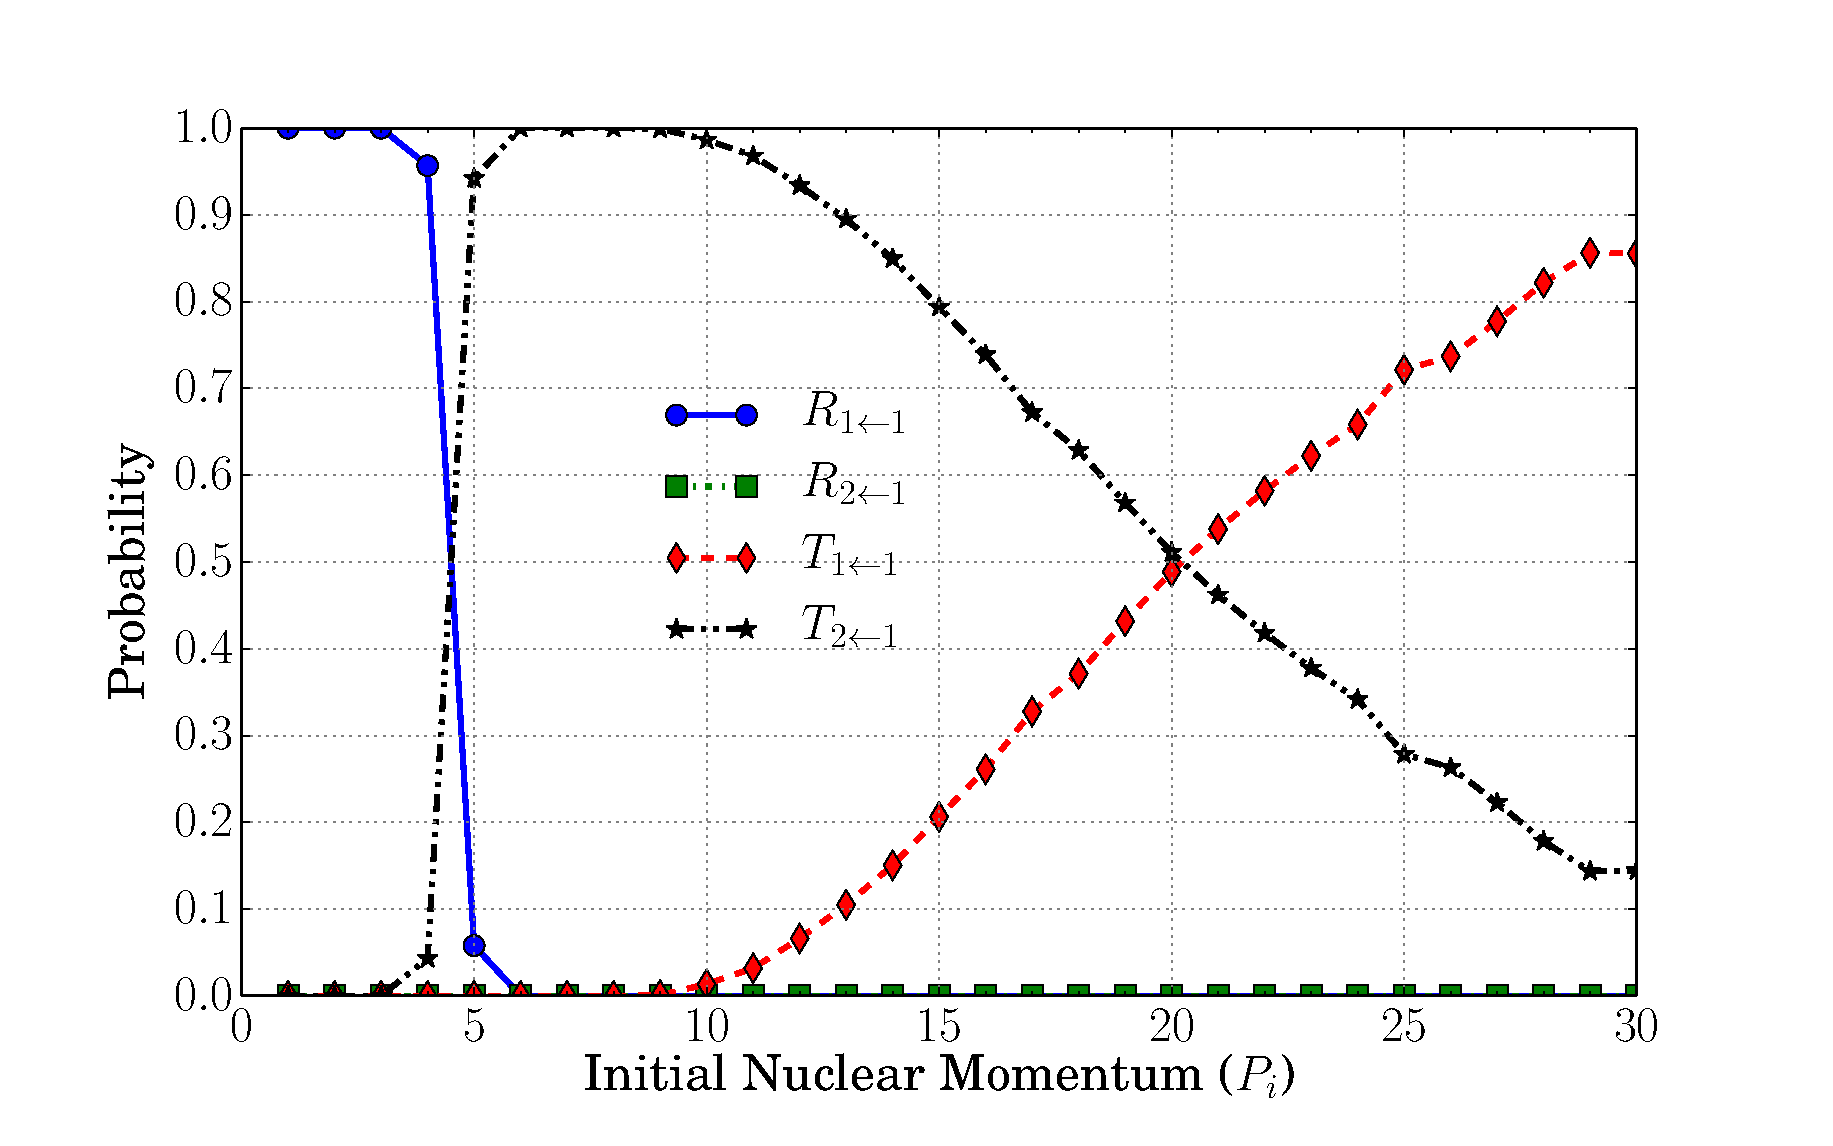
\includegraphics[width=\textwidth]{sc_prob_1o5ip.eps}
\vspace{-0.3cm}
\caption{{\fontsize{7}{8}\selectfont $ i = 1 $, $ h = (5P_{i})^{-1} $.}}
\label{f:sc1o5ip}
\end{subfigure}
~
\begin{subfigure}[t]{0.45\textwidth}
\centering
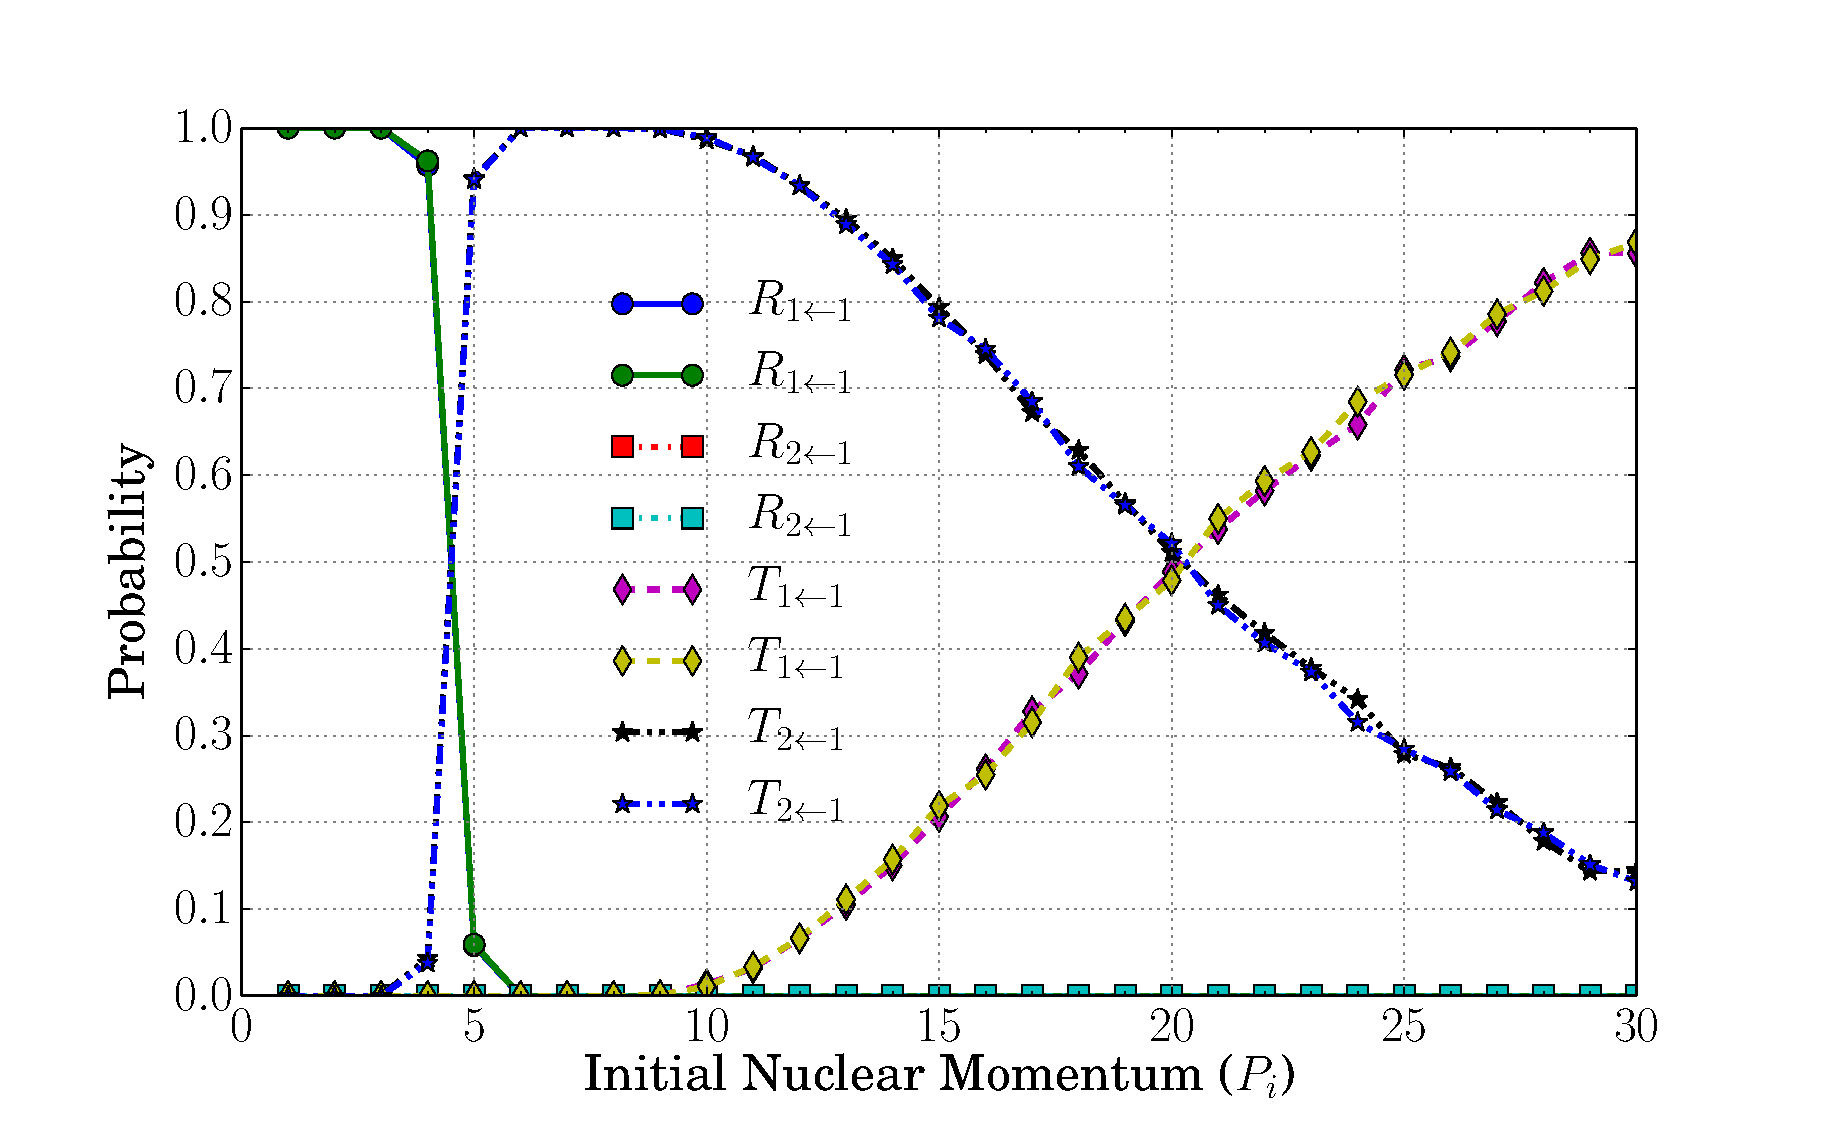
\includegraphics[width=\textwidth]{sc_prob_1oip_vs_1o5ip.eps}
\vspace{-0.35cm}
\caption{{\fontsize{7}{8}\selectfont $ i = 1 $, comparison between $ h = (5P_{i})^{-1} $ (1\textsuperscript{st} in lengend) and $ h = P_{i}^{-1} $.}}
\label{f:sccomp}
\end{subfigure}
\\[-0.3cm]
\begin{subfigure}[t]{0.45\textwidth}
\centering
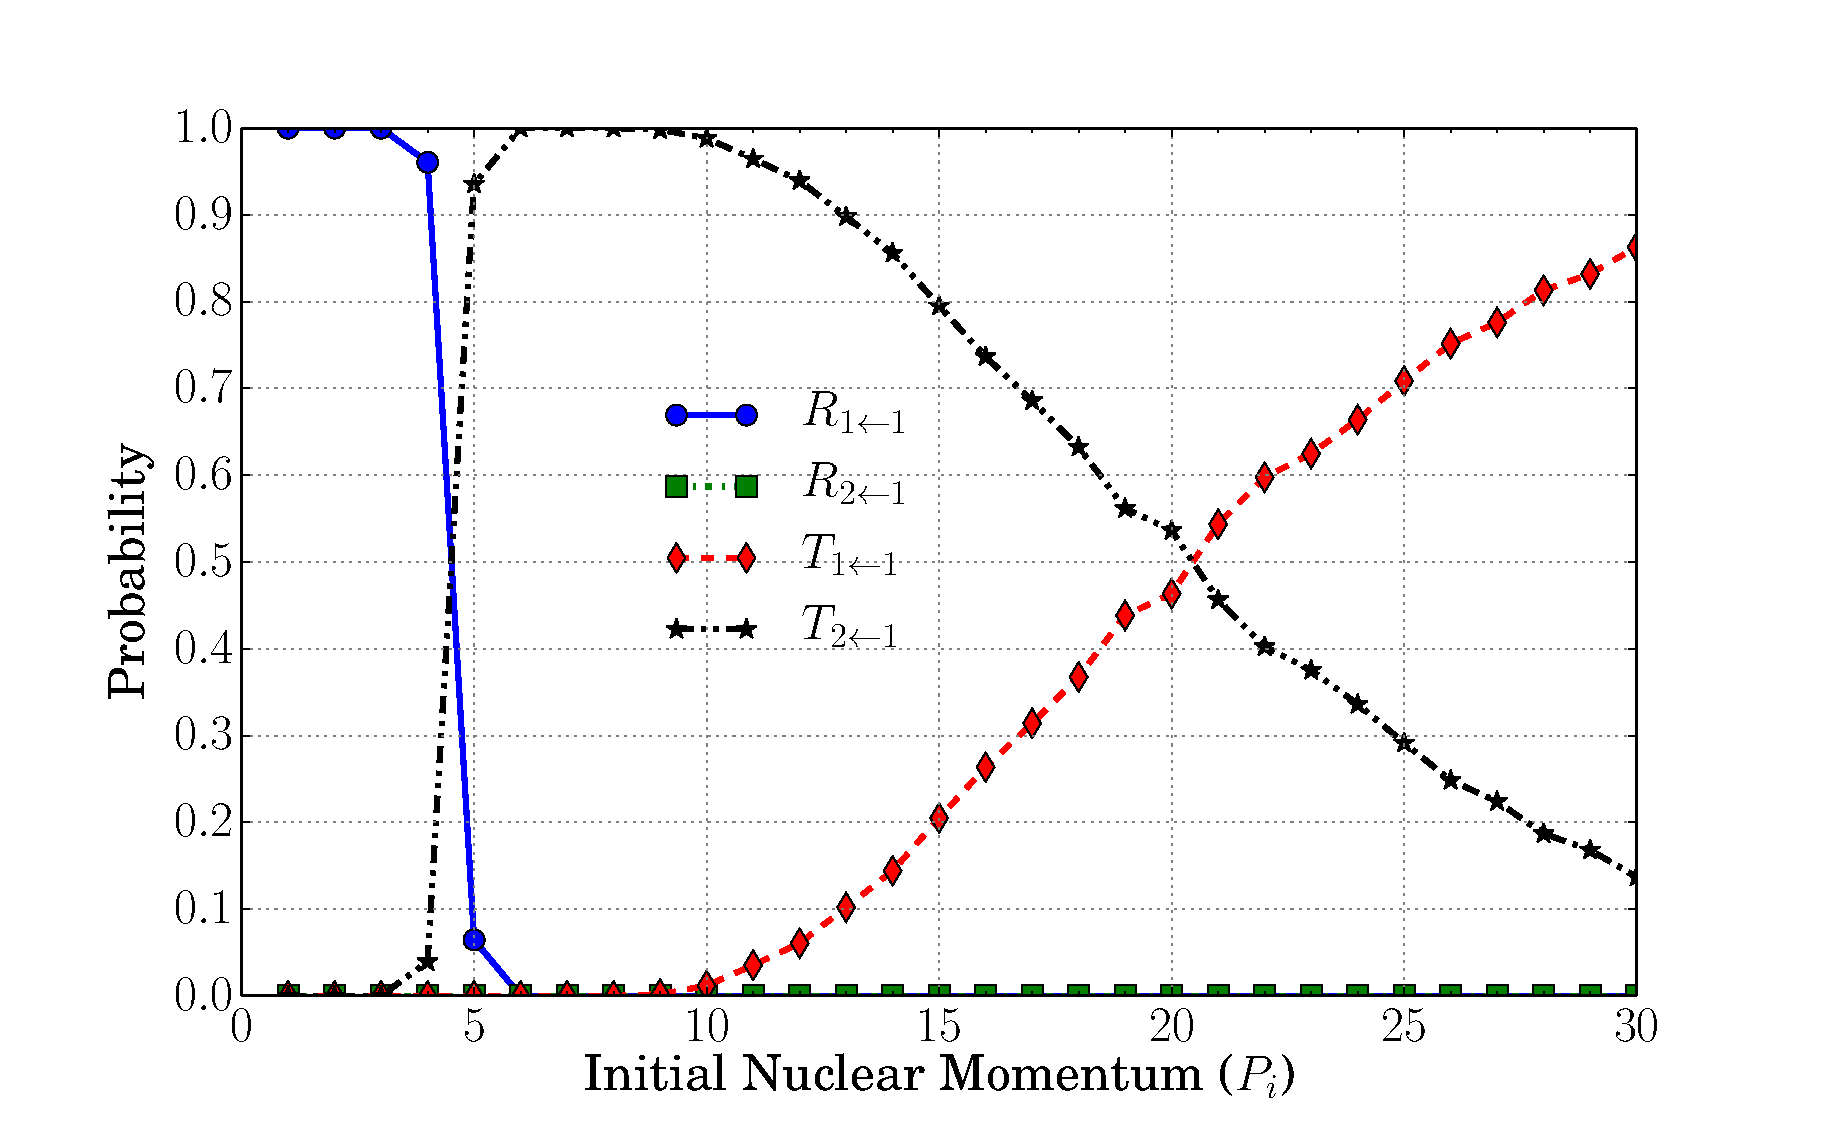
\includegraphics[width=\textwidth]{sc_prob_parallel.eps}
\vspace{-0.35cm}
\caption{{\fontsize{7}{8}\selectfont Parallel calculations, 2 nuclei, $ i = 1 $, $ h=(5P_{i})^{-1} $.}}
\label{f:scpar}
\end{subfigure}
~
\begin{subfigure}[t]{0.45\textwidth}
\centering
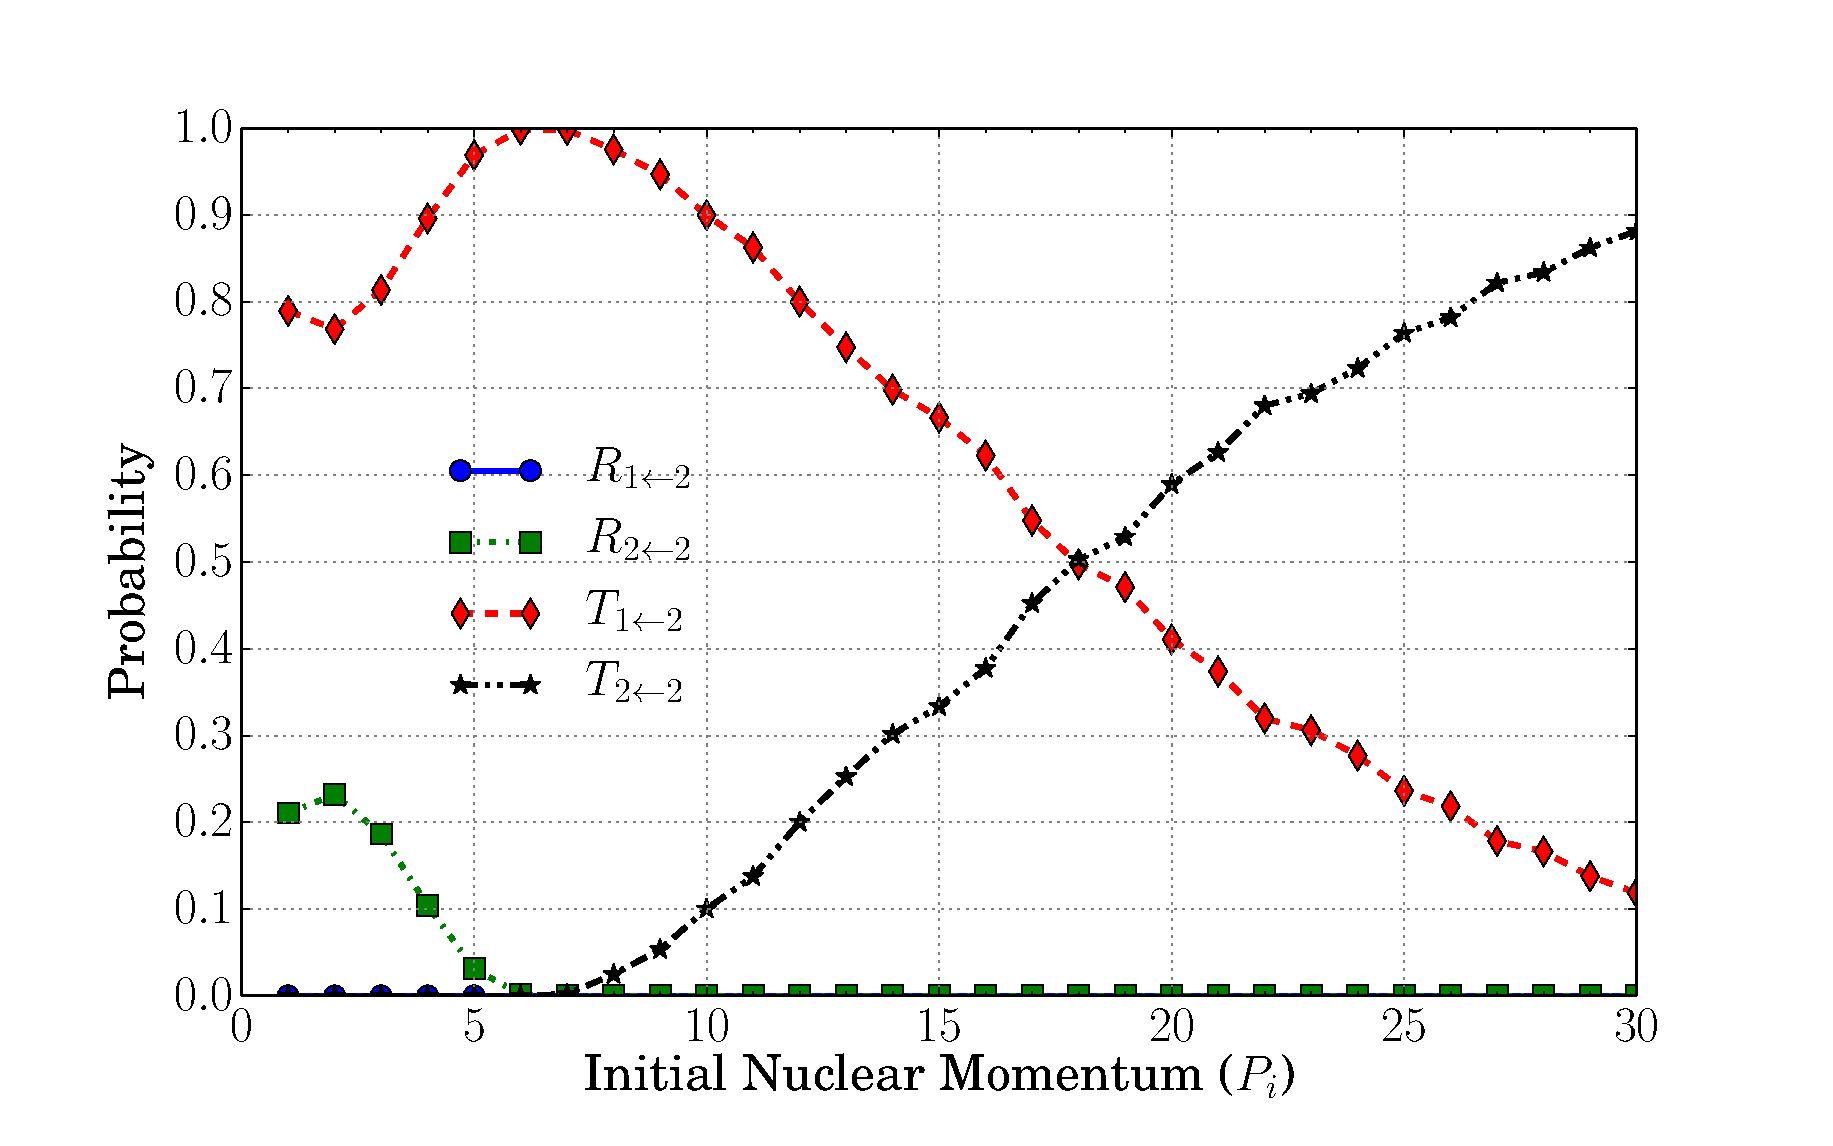
\includegraphics[width=\textwidth]{sc_prob_i2.eps}
\caption{{\fontsize{7}{8}\selectfont $ i = 2 $, $ h = (0.012P_{i})^{-1} $.}}
\label{f:sci2}
\end{subfigure}
\vspace{-0.47cm}
\caption{Transition Probabilities.}
\end{figure}
}{\stepcounter{figure}}
\end{frame}

\subsection{Double Avoided Crossing}
\begin{frame}
\frametitle{Double Avoided Crossing}
%\vspace{-0.33cm}
\alt<1>{
\begin{figure}
\centering
\begin{subfigure}[t]{0.48\textwidth}
\centering
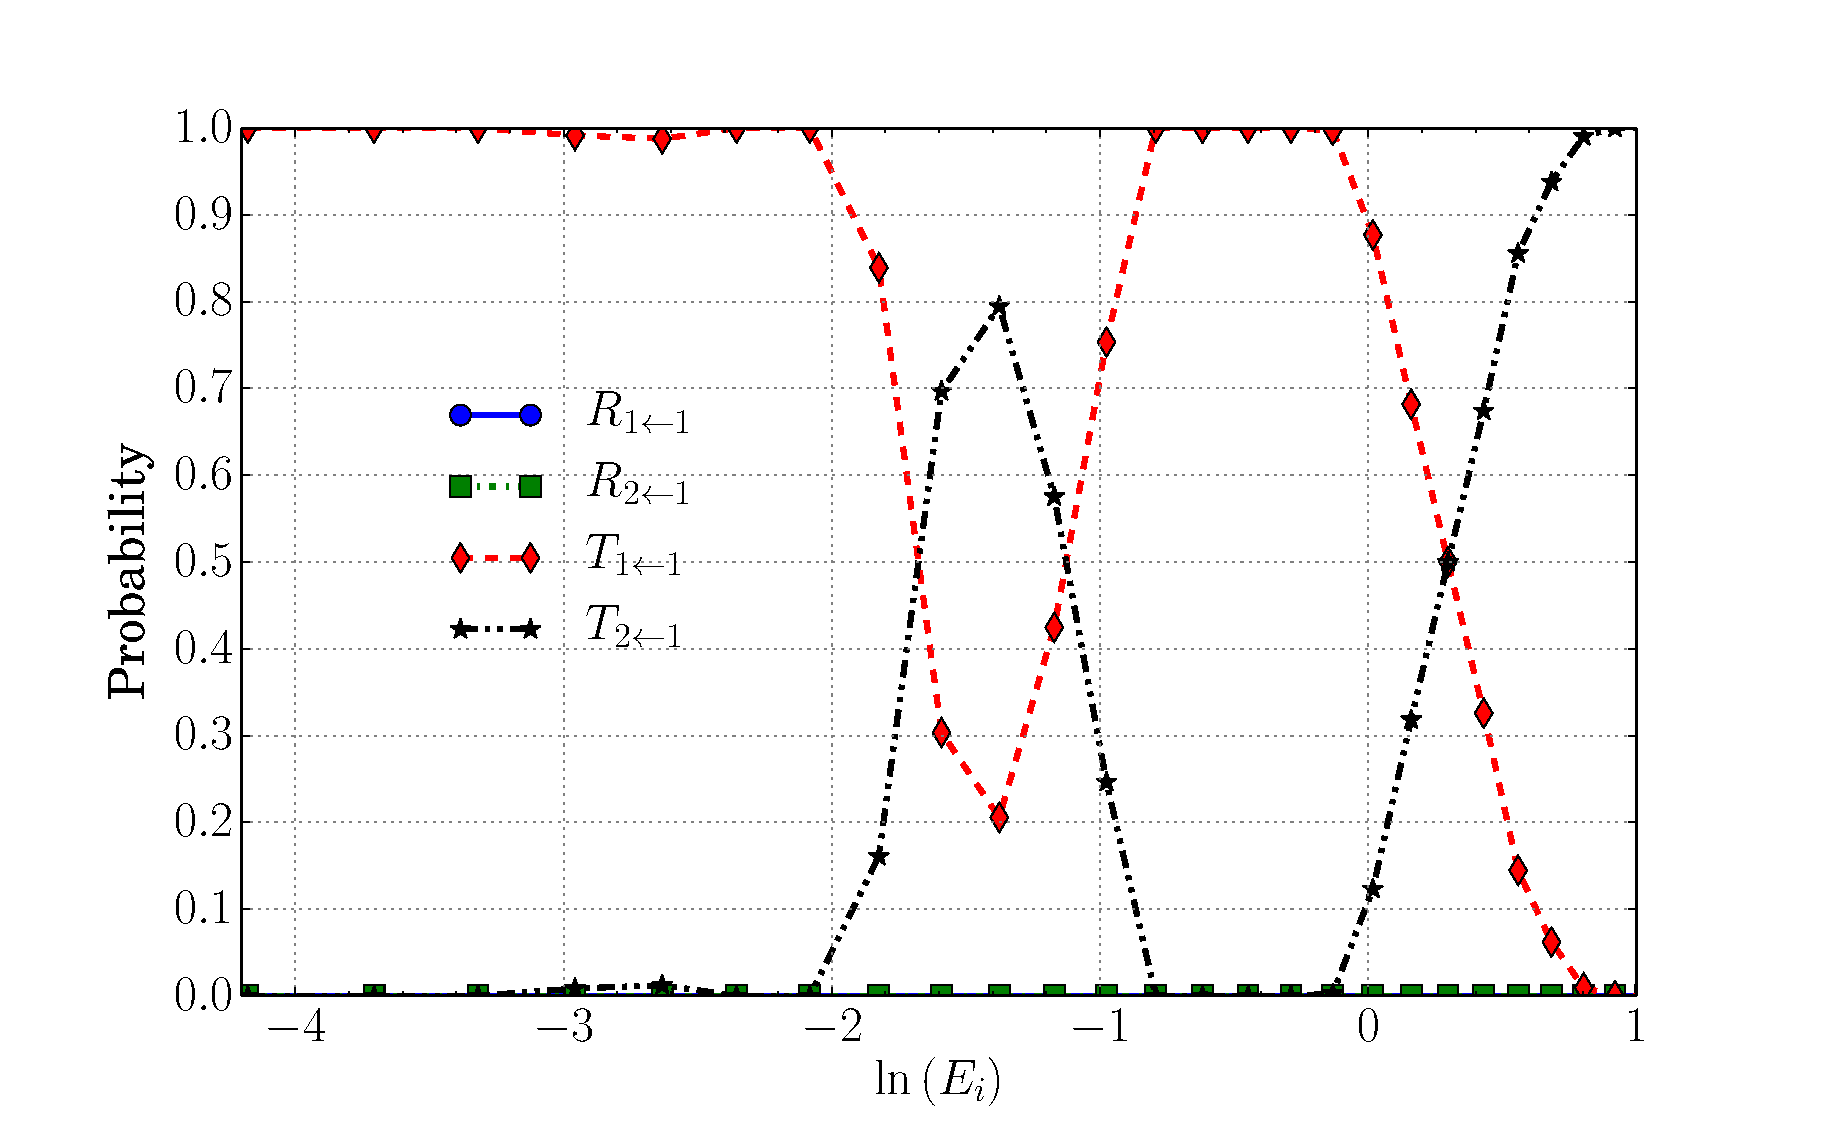
\includegraphics[width=\textwidth]{dc_prob_parallel.eps}
\caption{$ i = 1 $, $ h = (0.0125P_{i})^{-1} $.}
\label{f:dcpar}
\end{subfigure}
~
\begin{subfigure}[t]{0.48\textwidth}
\centering
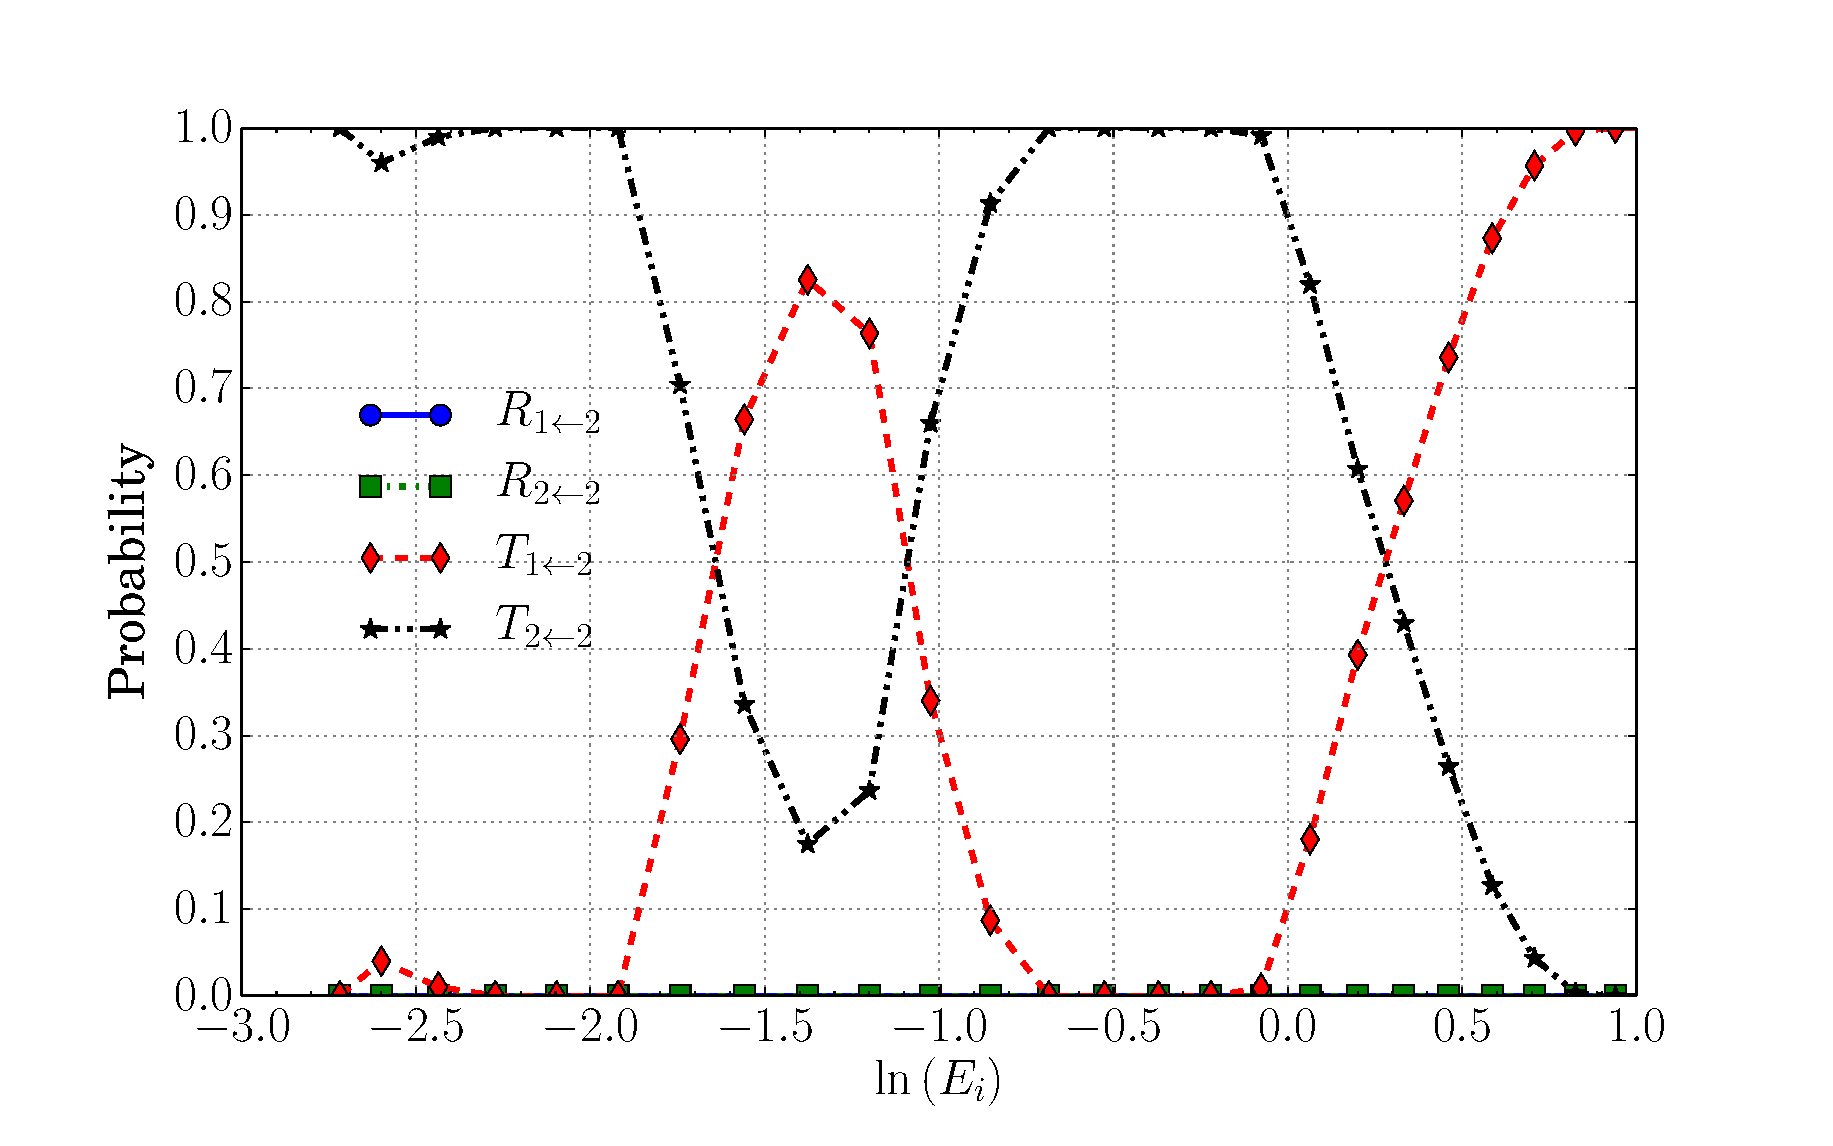
\includegraphics[width=\textwidth]{dc_prob_i2.eps}
\caption{$ i = 2 $, $ h = (0.0125P_{i})^{-1} $.}
\label{f:dci2}
\end{subfigure}
\caption{Transition probabilities.}
\end{figure}
}{\stepcounter{figure}}
\end{frame}

\subsection{Extended Coupling}
\begin{frame}
\frametitle{Extended Coupling}
%\vspace{-0.33cm}
\alt<1>{
\begin{figure}
\begin{subfigure}[t]{0.48\textwidth}
\centering
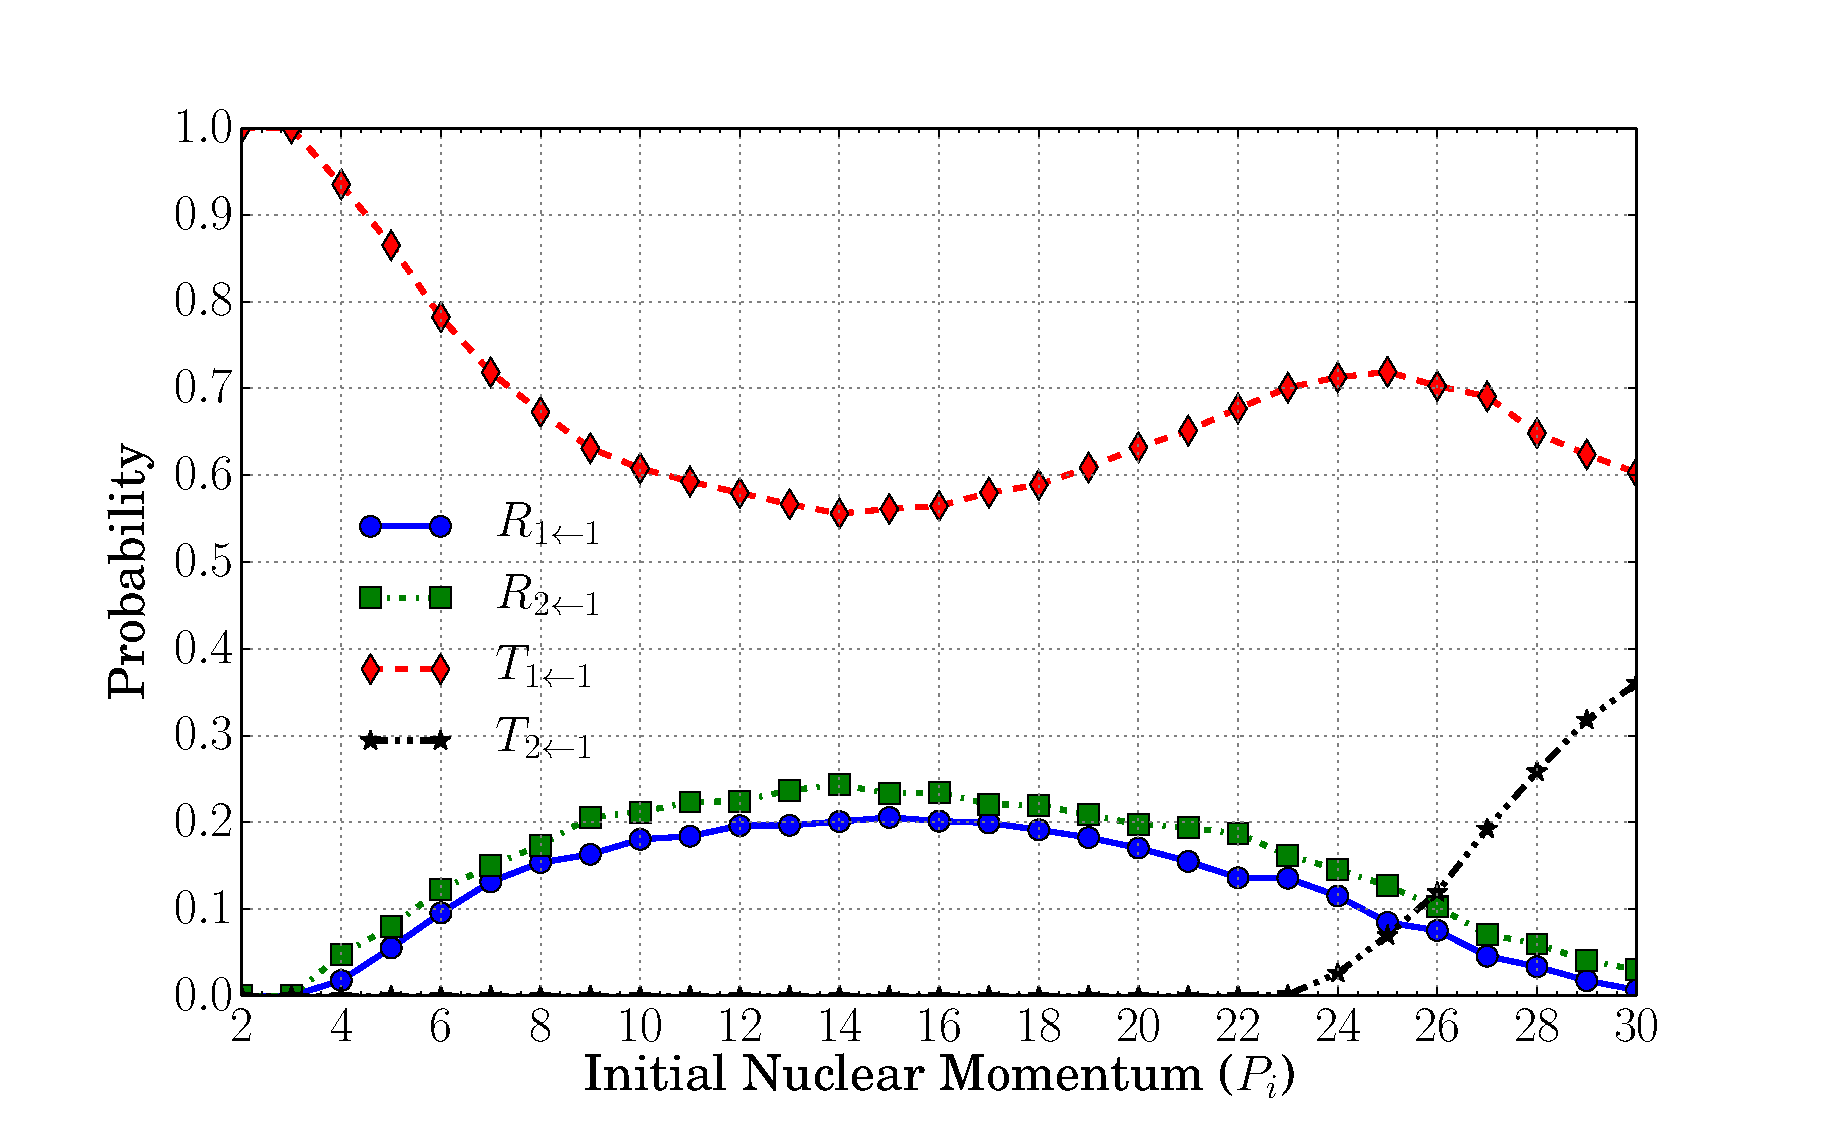
\includegraphics[width=\textwidth]{ec_prob_lh_mean.eps}
\caption{$ i = 1 $, $ h=(0.10125P_{i})^{-1} $, $ 30000 $ MC reps.}
\label{f:eclhmean}
\end{subfigure}
~
\begin{subfigure}[t]{0.48\textwidth}
\centering
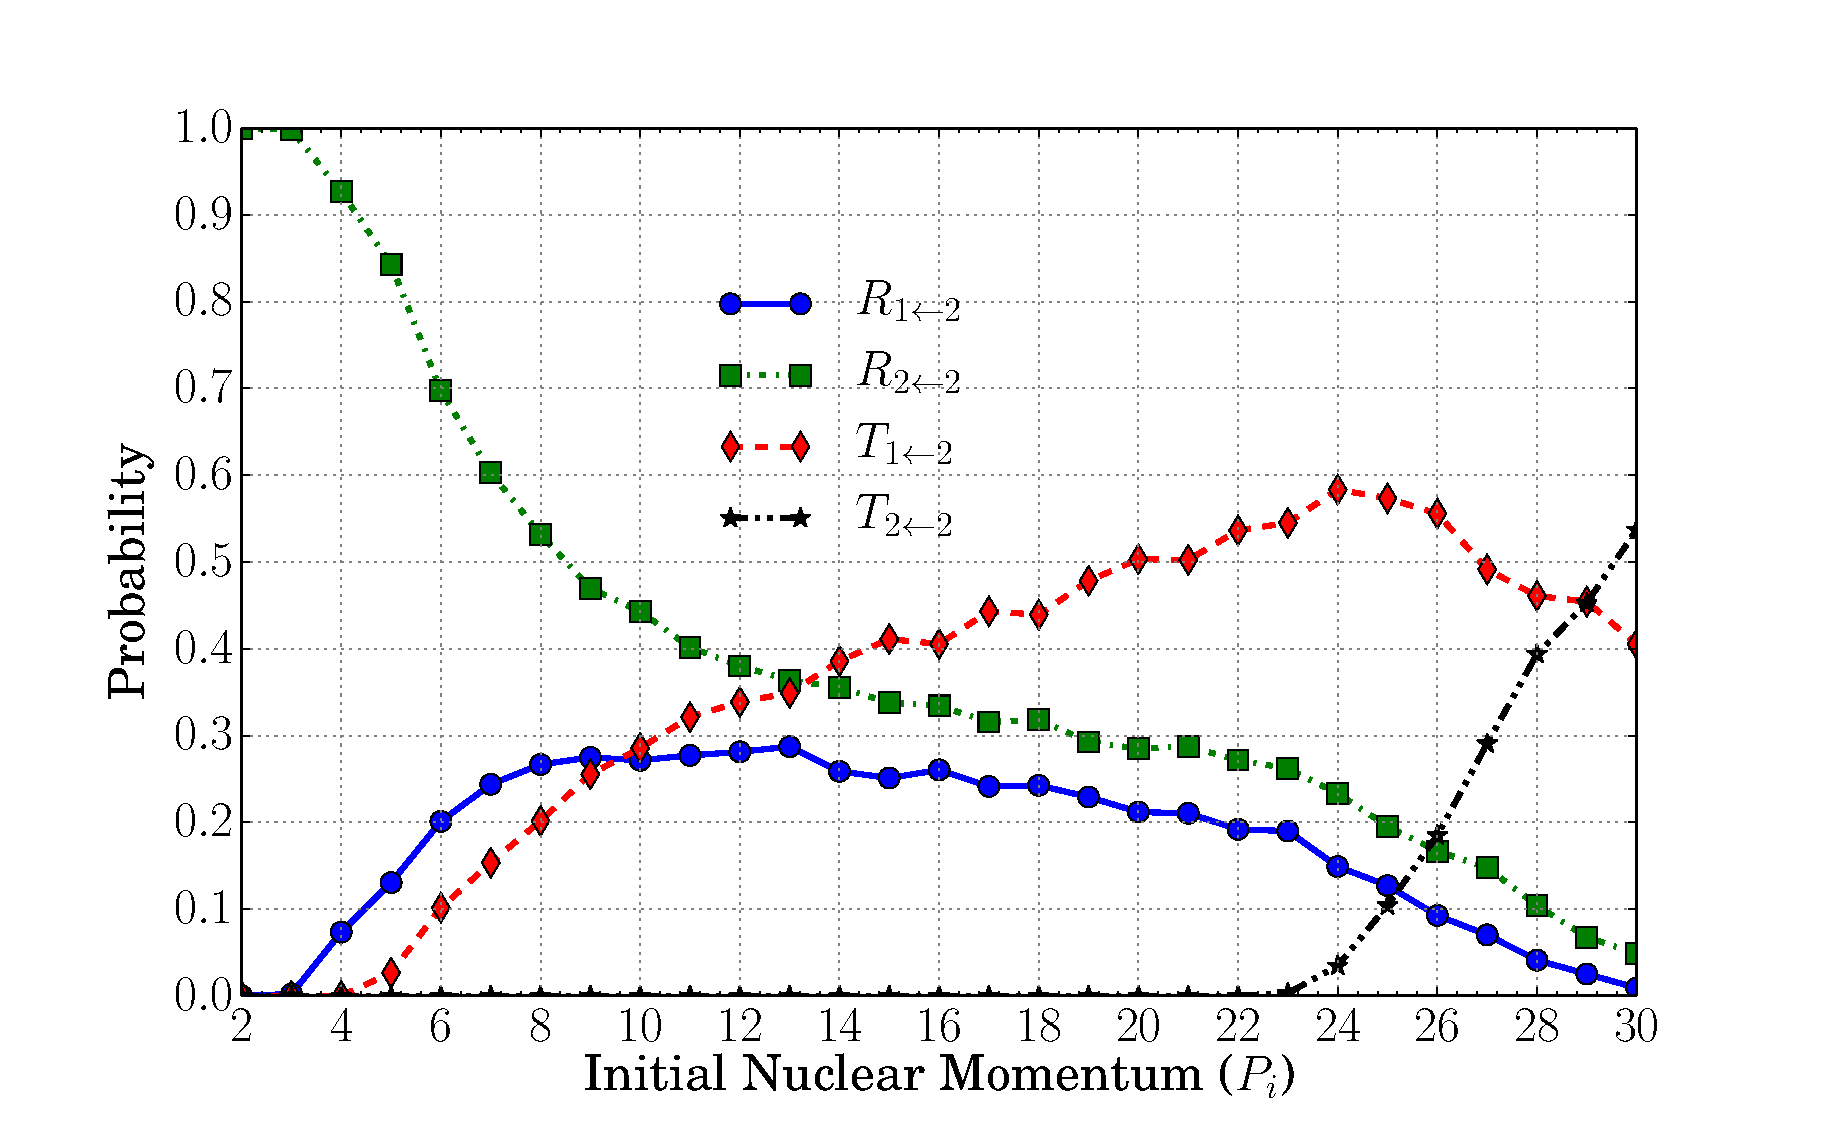
\includegraphics[width=\textwidth]{ec_prob_i2.eps}
\caption{$ i = 2 $, $ h=(0.10125P_{i})^{-1} $.}
\label{f:eci2}
\end{subfigure}
\caption{Transition probabilities.}
\end{figure}
}{\stepcounter{figure}}
\end{frame}

\subsection{Condensed-Phase Spin-Boson Model}
\begin{frame}
\frametitle{Condensed-Phase Spin-Boson Model}
%\vspace{-0.33cm}
\alt<1>{
\begin{figure}
\centering
\begin{subfigure}[t]{0.48\textwidth}
\centering
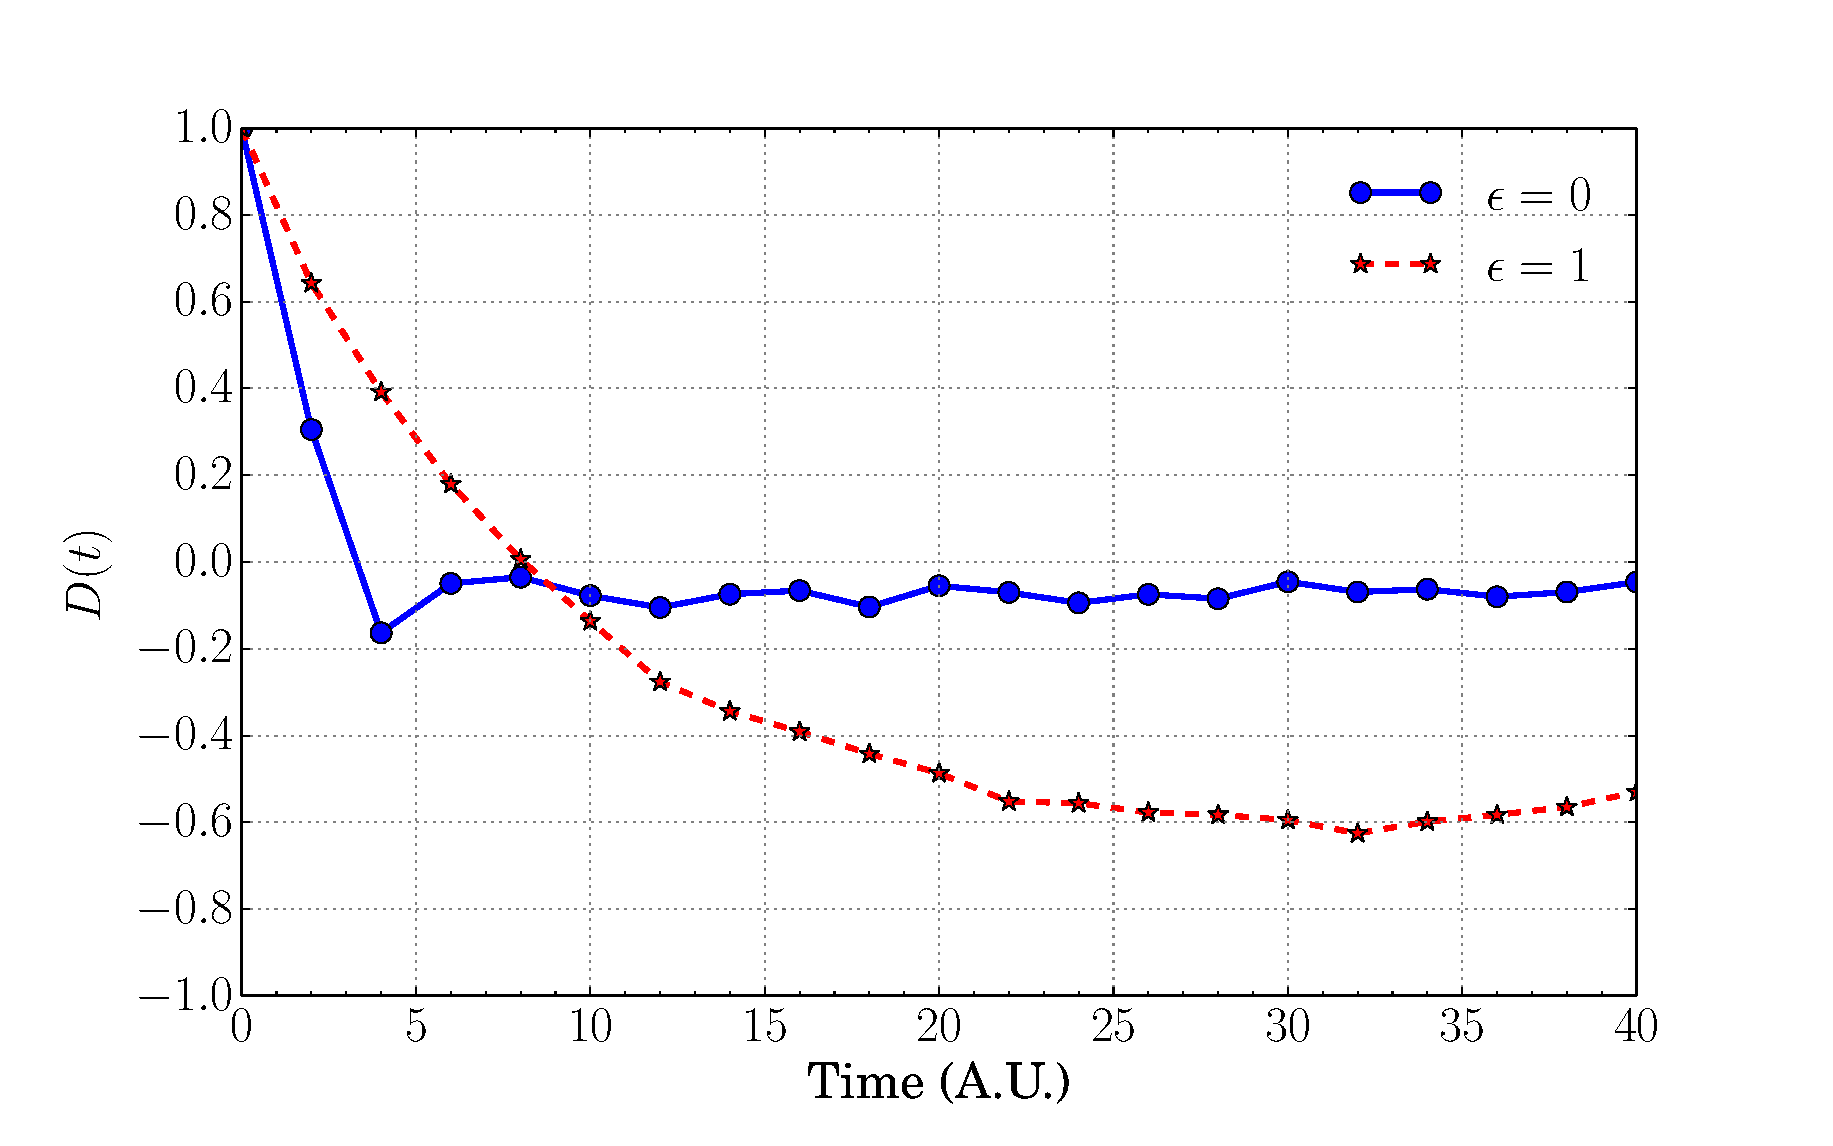
\includegraphics[width=\textwidth]{spin_boson_e11.eps}
\caption{$ i = 1 $, $ h = 0.01 $.}
\label{f:sb11}
\end{subfigure}
~
\begin{subfigure}[t]{0.48\textwidth}
\centering
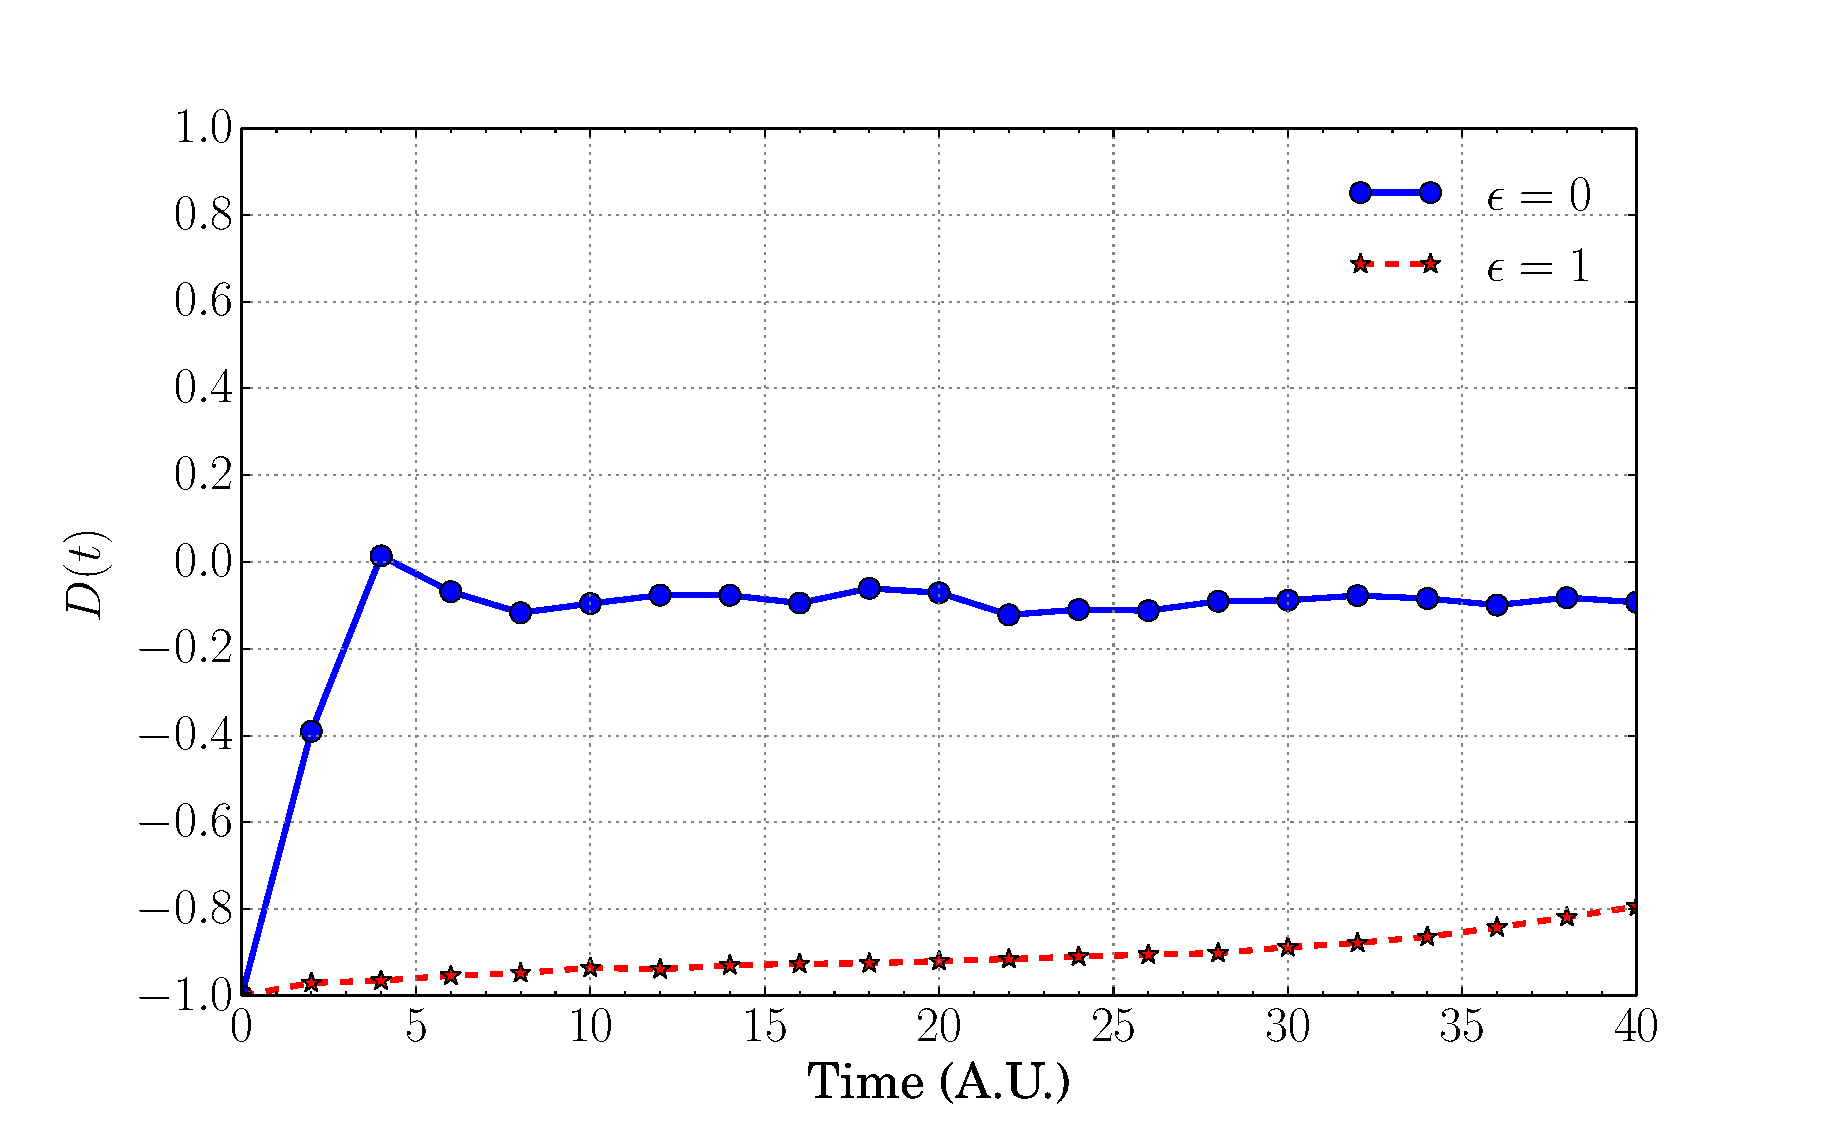
\includegraphics[width=\textwidth]{spin_boson_e12.eps}
\caption{$ i = 2 $. For the symmetric problem, $ h = 0.1 $ and MC reps $ = 5000 $. For the asymmetric one, $ h = 0.01 $ and MC reps $ = 30000 $.}
\label{f:sb12}
\end{subfigure}
\caption{Symmetric ($ \epsilon = 0 $) and asymmetric ($ \epsilon = 1 $) problems. $ \alpha = 0.09$, $\beta = 0.25$, $\Delta = (2.5)^{-1}$.}
\end{figure}
}{\stepcounter{figure}}

\alt<2>{
\begin{figure}
\begin{subfigure}[t]{0.48\textwidth}
\centering
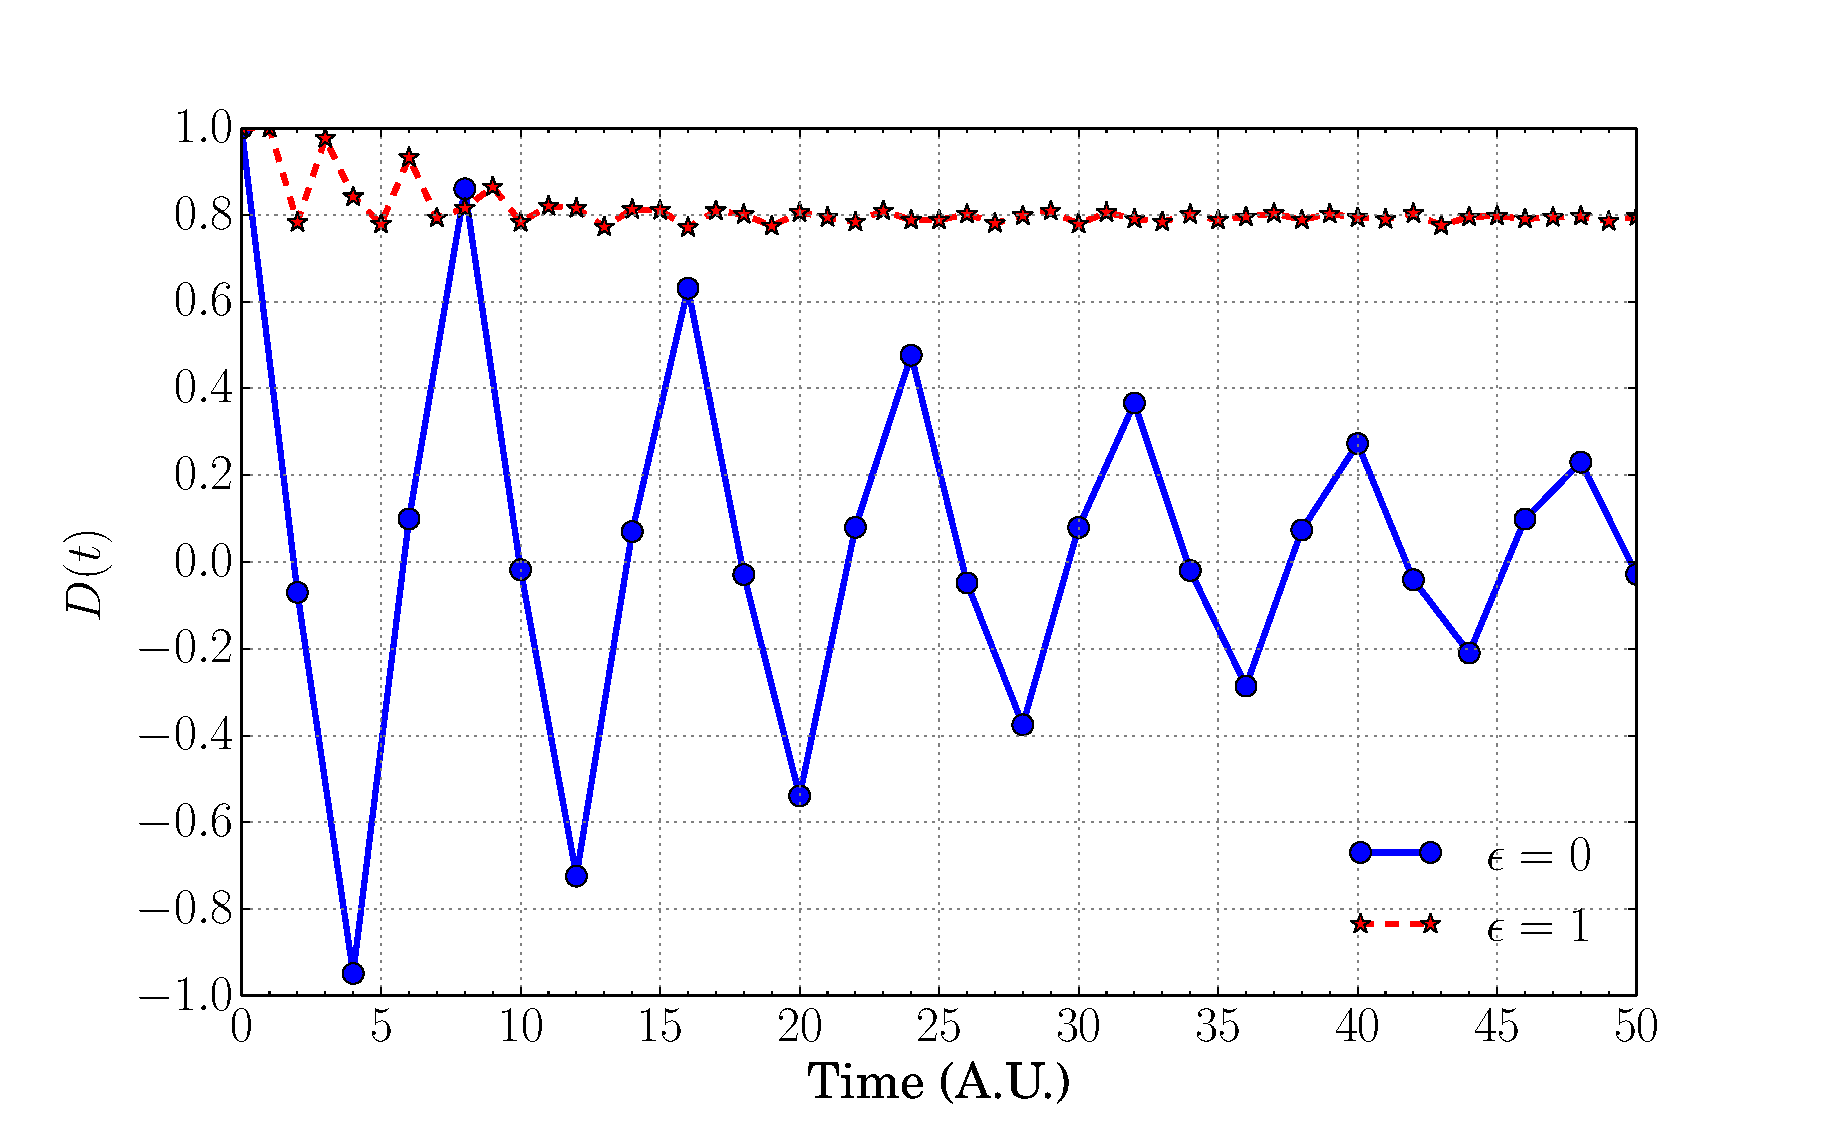
\includegraphics[width=\textwidth]{spin_boson_e21.eps}
\caption{$ i = 1 $. For the symmetric problem, $ h = 0.1 $ and MC reps $ = 5000 $. For the asymmetric one, $ h = 0.05 $ and MC reps $ =30000 $.}
\label{f:sb21}
\end{subfigure}
~
\begin{subfigure}[t]{0.48\textwidth}
\centering
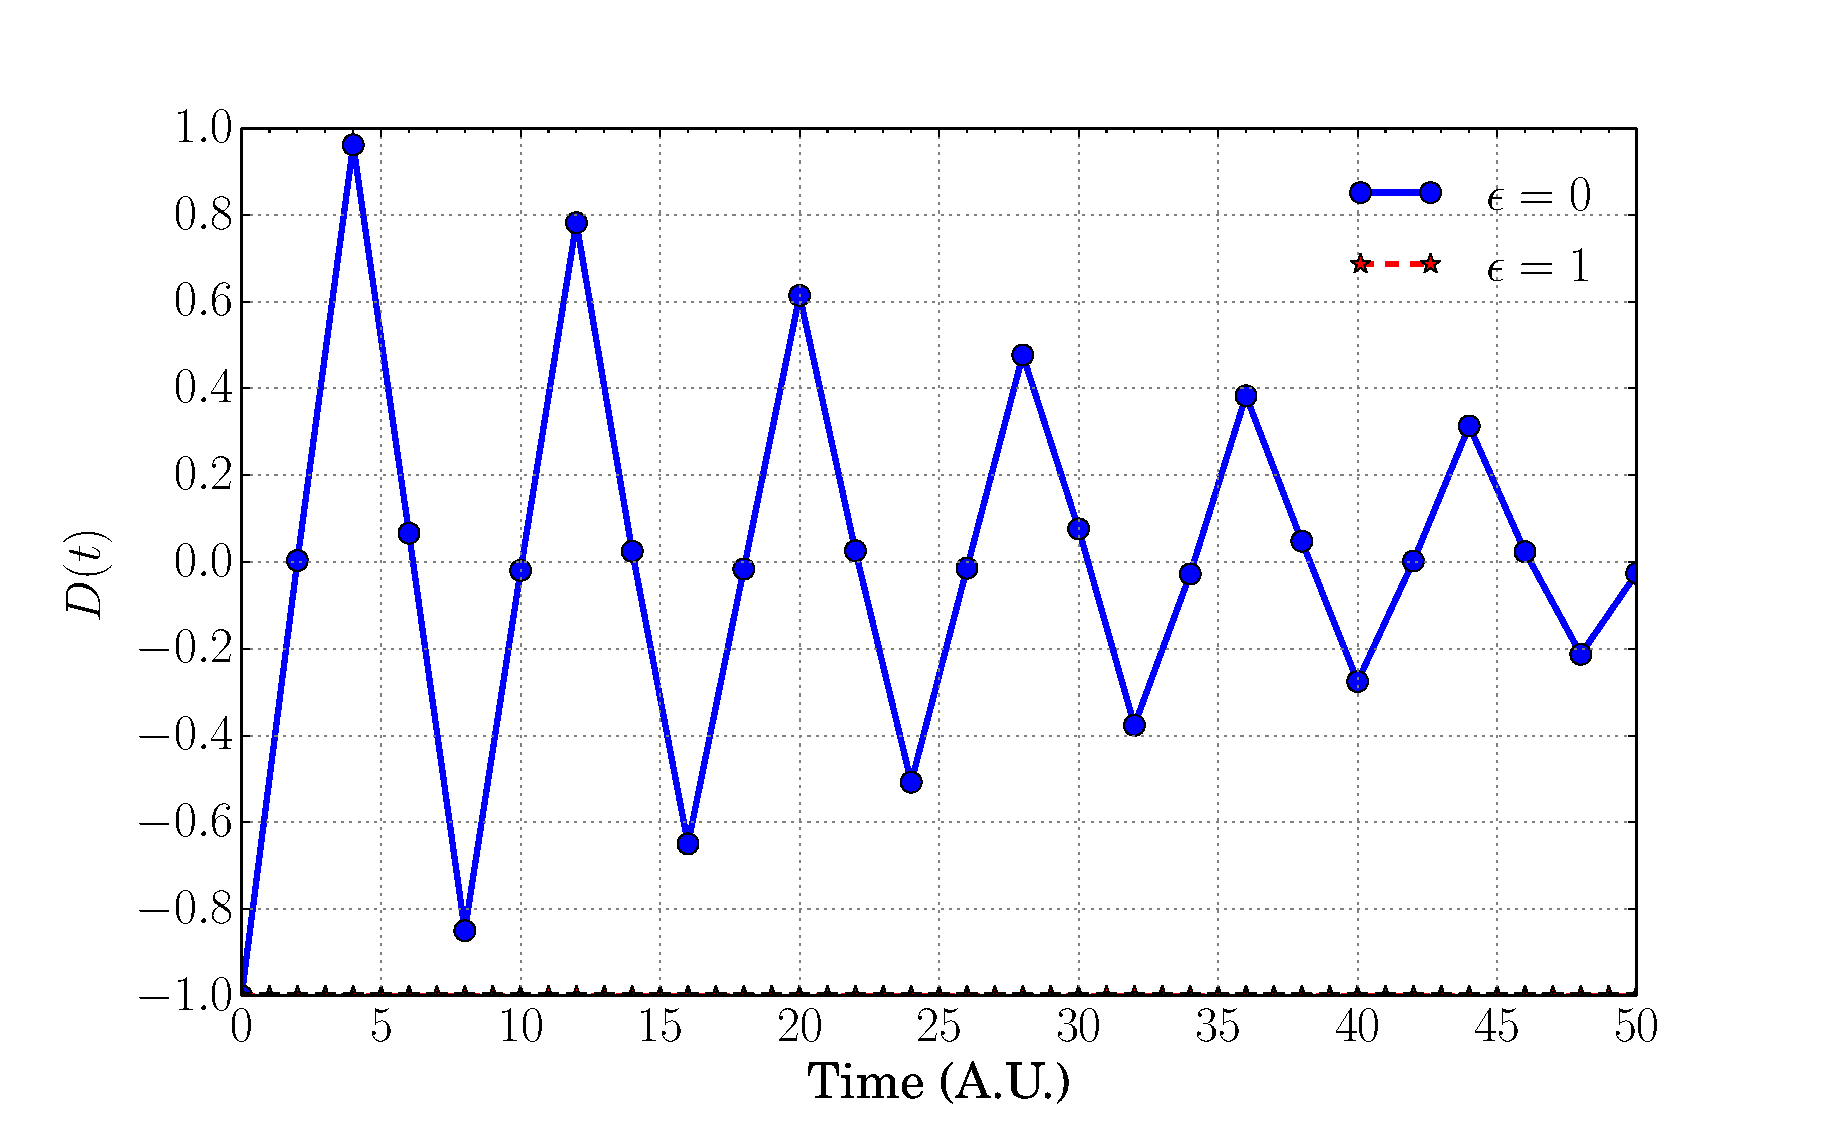
\includegraphics[width=\textwidth]{spin_boson_e22.eps}
\caption{$ i = 2 $. For the symmetric problem, $ h = 0.1 $ and MC reps $ = 5000 $. For the asymmetric one, $ h = 0.05 $ and MC reps $ =30000 $.}
\label{f:sb22}
\end{subfigure}
\caption{Symmetric ($ \epsilon = 0 $) and asymmetric ($ \epsilon = 1 $) problems. $ \alpha = 0.1$, $\beta = 12.5$, $\Delta = (2.5)^{-1}$.}
\end{figure}
}{\stepcounter{figure}}
\end{frame}

\section{Conclusions}
\subsection{Conclusion}
\begin{frame}
\frametitle{Conclusion}
\begin{itemize}
\item The model was successfully implemented in \textsc{fortran 2008}.
\item The code was validated with four simple model systems.
\item New results for all four systems were obtained.
\item The model's inner workings can be appreciated through the calculated trajectories found in the Appendix.
\end{itemize}
\end{frame}

\subsection{Future Work}
\begin{frame}
\frametitle{Future Work}
\begin{itemize}
\item Modify the code so it can read input files. Trivial with \texttt{\textcolor{green}{read}(\textcolor{grey}{*},\textcolor{grey}{*})} and \texttt{\textcolor{purple}{module}}.
\item Make use of an adaptive integration algorithm. Trivial.
\item Generalise the code so it can be applied to arbitrary sytems. Trivial with \texttt{\textcolor{green}{read}(\textcolor{grey}{*},\textcolor{grey}{*})} and \texttt{\textcolor{purple}{module}}.
\item Eliminate the need for analytic PES. Not trivial.
\item Apply the model to real systems. Not trivial.
\end{itemize}
\end{frame}

\appendix
\begin{frame}
\frametitle{References}
\begin{thebibliography}{10}
\bibitem{project}
Cotton, Stephen J and Miller, William H.
\newblock Symmetrical windowing for quantum states in quasiclassical trajectory simulations: Application to electronically non-adiabatic processes.
\newblock \emph{The Journal of Chemical Physics}, vol. 139, no. 23, p. 234112, 2013.
\bibitem{tully}
Tully, John C.
\newblock \emph{The Journal of Chemical Physics}, vol. 93, no. 2, pp. 1061--1071, 1990.
\bibitem{spin-boson}
Stock, Gerhard.
\newblock A semiclassical self-consistent-field approach to dissipative dynamics: The spin--boson problem.
\newblock \emph{The Journal of Chemical Physics}, vol 103, no. 4, pp. 1561--1573, 1995.
\end{thebibliography}
\end{frame}

\section{Acknowledgements}
\begin{frame}
\only<1>{
\begin{multicols}{2}
\begin{itemize}
\item Prof. John F. Stanton
\item Prof. Marcelo Videa Vargas
\item Julio L. Palma, PhD.
\item Mr. Casserly
\item Prof. Bernard J. Micheli Masson
\item Prof. Anatoly Kolomeisky
\item MSc. Hamid Teimouri
\item Prof. Víctor Jiménez Pérez
\item Prof. Víctor Rosas García
\item Prof. Jesús Valencia Gallegos
\item Prof. Julio César Gutiérrez Vega
\item Rodrigo Chan Navarro, PhD.
\item Concepción ``Conny'' García, PhD.
\item Professors of the chemistry department.
\item Pedrito, Ángel, Alex
\item Irving Rodríguez.
\item Dámaris, Bere Garza
\end{itemize}
\end{multicols}
}
\only<2>{
\begin{center}
\Huge{\centerline{My friends\dots}}
\end{center}
}
\only<3>{
\Huge{\centerline{My family\dots}}
}
\only<4>{
\Huge{\centerline{Cheers!}}
}
%\only<5>{
%fotos
%}
\end{frame}

\section{Questions}
\begin{frame}
\Huge{\centerline{?}}
\end{frame}

\section{Appendix}
\subsection{Classical Mechanics}
\begin{frame}
\frametitle{Classical Mechanics}
\alt<1>{
\framesubtitle{Newtonian Fromalism}
\begin{subequations}
\begin{align}
F &= ma = m \dif{^{2} f(\mathbf{x},t)}{t^{2}}\\
F &= -\nabla V
\end{align}
\end{subequations}
\begin{itemize}
\item Formulated around vectors.
\item Rapidly increasing complexity.
\item Non-generalised coordinates.
\end{itemize}
}{\stepcounter{equation}}

\alt<2>{
\framesubtitle{Lagrangian Formalism}
\begin{subequations}
\begin{align}
L &= T - V \\
\mathcal{S}[\mathbf{q}(t)] &=  \int_{t_1}^{t_2} L[\mathbf{q}(t),\dot{\mathbf{q}}(t),t] \textrm{d}t\\
\dpar{L}{q_{j}} & = \dif{}{t}\left(\dpar{L}{\dot{q}_{j}}\right)
\end{align}
\end{subequations}
\begin{itemize}
\item Where $ T \equiv $ kinetic energy, $ V \equiv $ potential energy, $ q_{j} \equiv $ generalised position, $ \dot{q}_{j} = \dif{q_{j}}{t} \equiv $ generalised velocity.
\item Partial differential equations.
\item Less geometrically-driven than its Newtonian counterpart.
\item Non-trivial solutions.
\end{itemize}
}{\stepcounter{equation}}

\alt<3>{
\framesubtitle{Hamiltonian Formalism}
\begin{subequations}
\begin{align}
H = \sum\limits_{j} \dot{q}_{j} \dpar{L}{\dot{q}_{j}} & - L = \sum\limits_{j} \dot{q}_{j} p_{j} - L\\
H &= T + V\\
\dpar{H}{q_{j}} = -\dot{p}_{j}\quad,\quad &\dpar{H}{p_{j}} = \dot{q}_{j}\quad,\quad \dpar{H}{t} = -\dpar{L}{t}
\end{align}
\end{subequations}
\begin{itemize}
\item Where $ p_{j} \equiv $ generalised momentum.
\item Ordinary differential equation systems.
\item Trivial solutions.
\end{itemize}
}{\stepcounter{equation}}
\end{frame}

\subsection{Quantum Mechanics}
\begin{frame}
\frametitle{Quantum Mechanics}
\begin{subequations}
\begin{align}
E \Psi &= \hat{H} \Psi\\
\hat{H} &= -\frac{\hbar}{2\mu} \nabla^{2} + V(\bm{r})
\end{align}
\end{subequations}

\begin{subequations}
\begin{align}
i \hbar \frac{\partial}{\partial t}\Psi &= \hat{H}\Psi\\
\hat{H} &= -\frac{\hbar}{2\mu} \nabla^{2} + V(\bm{r},t)
\end{align}
\end{subequations}
\end{frame}

\subsection{Diabatic Hamiltonian in Cartesian Variables}
\begin{frame}
\frametitle{Diabatic Hamiltonian in Cartesian Variables}
\alt<1>{
\framesubtitle{$ F = 2 $}
\begin{align}\label{e:diab_ham_f=2}
H(\bm{P}, \bm{R}, \bm{p}, \bm{x})
&=\frac{\bm{P}^{2}}{2\mu}+\frac{1}{2}(H_{11}(\bm{R})+H_{22}\bm{R})\\
&+\frac{1}{2}(H_{11}(\bm{R})-H_{22}(\bm{R}))\cdot\left(\frac{1}{2}p_{1}^{2}+\frac{1}{2}x_{1}^{2}-\frac{1}{2}p_{2}^{2}-\frac{1}{2}x_{2}^{2}\right)\nnum
&+H_{12}(\bm{R})\cdot(p_{1}p_{2}+x_{1}x_{2}) \nonumber
\end{align}
}{\stepcounter{equation}}

\alt<2>{
\framesubtitle{Equations of Motion $( F = 2 )$}
\begin{subequations}
\begin{align}\label{e:diab_motion_f=2}
&\dot{\bm{R}} = \frac{\bm{P}}{\mu}\\
&\dot{\bm{P}} = 
-\frac{1}{2}\dpara{H_{11}}{\bm{R}}{H_{22}}{\bm{R}}-\frac{1}{4}\dpars{H_{11}}{\bm{R}}{H_{22}}{\bm{R}}(p_{1}^{2}+x_{1}^{2}-p_{2}^{2}-x_{2}^{2})\nnum
&\qquad-\dpar{H_{12}}{\bm{R}}(p_{1}p_{2}+x_{1}x_{2})\\
&\dot{x}_{1} = \frac{1}{2}p_{1}(H_{11}-H_{22})+p_{2}H_{12}\\
&\dot{p}_{1} = -\frac{1}{2}x_{1}(H_{11}-H_{22})-x_{2}H_{12}\\
&\dot{x}_{2} = -\frac{1}{2}p_{2}(H_{11}-H_{22})+p_{1}H_{12}\\
&\dot{p}_{2} = \frac{1}{2}x_{2}(H_{11}-H_{22})-x_{1}H_{12}
\end{align}
\end{subequations}
}{\stepcounter{equation}}
\end{frame}

\subsection{Adiabatic Hamiltonian in Cartesian Variables}
\begin{frame}
\frametitle{Adiabatic Hamiltonian in Cartesian Variables}
\alt<1>{
\framesubtitle{$ F = 2 $}
\begin{align}
& H(\bm{P}, \bm{R}, \bm{p}, \bm{x}) = 
\frac{|\bm{P}+\nabla\bm{P}|^{2}}{2\mu}+\frac{1}{2}(E_{1}+E_{2})\\
& +\frac{1}{2} (E_{1}(\bm{R})-E_{2}(\bm{R}))\cdot\left(
\frac{1}{2}p_{1}^{2}+\frac{1}{2}x_{1}^{2}-\frac{1}{2}p_{2}^{2}-\frac{1}{2}x_{2}^{2}\right)\nonumber
\end{align}
}{\stepcounter{equation}}

\alt<2>{
\framesubtitle{Equations of Motion $( F = 2 )$}
\begin{subequations}
\begin{align}\label{e:adiab_motion_f=2}
&\dot{\bm{R}} = \frac{\bm{P}}{\mu}+\frac{1}{2\mu} 
\arctan\left(\frac{2H_{12}}{H_{11}-H_{22}}\right)(p_{1}x_{2}-p_{2}x_{1})\\
&\dot{\bm{P}} = -\left[\frac{\bm{P}}{\mu}+\frac{1}{2\mu}  
\arctan\left(\frac{2H_{12}}{H_{11}-H_{22}}\right)(p_{1}x_{2}-p_{2}x_{1})\right]\\
&\qquad\times\frac{\left[\dpar{H_{12}}{\bm{R}}(H_{11}-H_{22})+H_{12}\dpars{H_{22}}{\bm{R}}{H_{11}}{\bm{R}}\right](p_{1}x_{2}-p_{2}x_{1})}
{4H_{12}^{2}+(H_{11}-H_{22})^{2}}
\nnum
&\qquad-\frac{1}{4}\dpars{E_{1}}{\bm{R}}{E_{2}}{\bm{R}}(p_{1}^{2}+x_{1}^{2}-p_{2}^{2}-x_{2}^{2})
-\frac{1}{2}\dpara{E_{1}}{\bm{R}}{E_{2}}{\bm{R}}
\nnum
&\dot{x}_{1} = \left[\frac{\bm{P}}{2\mu}+\frac{1}{4\mu} 
\arctan\left(\frac{2H_{12}}{H_{11}-H_{22}}\right)(p_{1}x_{2}-p_{2}x_{1})\right]\nnum
&\qquad \times x_{2}\arctan\left(\frac{2H_{12}}{H_{11}-H_{22}}\right)+\frac{p_{1}}{2}(E_{1}-E_{2})
\end{align}
\end{subequations}
}{}

\alt<3>{
\framesubtitle{Equations of Motion $( F = 2 )$}
\begin{subequations}
\begin{align}\setcounter{equation}{3}
\dot{p}_{1} =& \left[\frac{\bm{P}}{2\mu}+\frac{1}{4\mu} 
\arctan\left(\frac{2H_{12}}{H_{11}-H_{22}}\right)(p_{1}x_{2}-p_{2}x_{1})\right]\nnum
& \times p_{2}\arctan\left(\frac{2H_{12}}{H_{11}-H_{22}}\right)-\frac{x_{1}}{2}(E_{1}-E_{2})
\\
\dot{x}_{2} =& -\left[\frac{\bm{P}}{2\mu}+\frac{1}{4\mu} 
\arctan\left(\frac{2H_{12}}{H_{11}-H_{22}}\right)(p_{1}x_{2}-p_{2}x_{1})\right]\nnum
& \times x_{1}\arctan\left(\frac{2H_{12}}{H_{11}-H_{22}}\right)-\frac{p_{2}}{2}(E_{1}-E_{2})
\\
\dot{p}_{2} =& -\left[\frac{\bm{P}}{2\mu}+\frac{1}{4\mu} 
\arctan\left(\frac{2H_{12}}{H_{11}-H_{22}}\right)(p_{1}x_{2}-p_{2}x_{1})\right]\nnum
& \times p_{2}\arctan\left(\frac{2H_{12}}{H_{11}-H_{22}}\right)+\frac{x_{2}}{2}(E_{1}-E_{2})
\end{align}
\end{subequations}
}{\stepcounter{equation}}
\end{frame}

\subsection{Single Avoided Crossing}
\begin{frame}
\frametitle{Single Avoided Crossing}
\alt<1>{
\framesubtitle{Diabatic PES Derivatives (DPES)}
\begin{subequations}
\begin{align}\label{e:dscpes}
\dpar{H_{11}}{R} & = 
\begin{cases}
A B e^{-B R} &\mbox{if } R \geq 0\\
A B e^{B R} &\mbox{if } R < 0
\end{cases}\\
\dpar{H_{22}}{R} &= -\dpar{H_{11}}{R}\\
\dpar{H_{12}}{R} &= \dpar{H_{21}}{R} = -2 C D e^{-D R^{2}} R
\end{align}
\end{subequations}
}{\stepcounter{equation}}

\alt<2>{
\framesubtitle{Adiabatic PES (APES)}
\begin{subequations}
\begin{align}\label{e:ascpes}
E_{1} &= -e^{-D R^{2}}
\sqrt{
C^{2} + e^{2 D R^{2}}
\begin{cases}
A^{2}(1 - e^{-B R})^{2} &\mbox{if } R\geq 0\\
A^{2}(1 - e^{B R})^{2} &\mbox{if } R<0
\end{cases}
}\\
E_{2} & = -E_{1}
\end{align}
\end{subequations}
}{\stepcounter{equation}}

\alt<3>{
\framesubtitle{Sample Trajectories ($ i=1 $).}
\vspace{-0.3cm}
\begin{figure}
\centering
\begin{subfigure}[t]{0.45\textwidth}
\centering
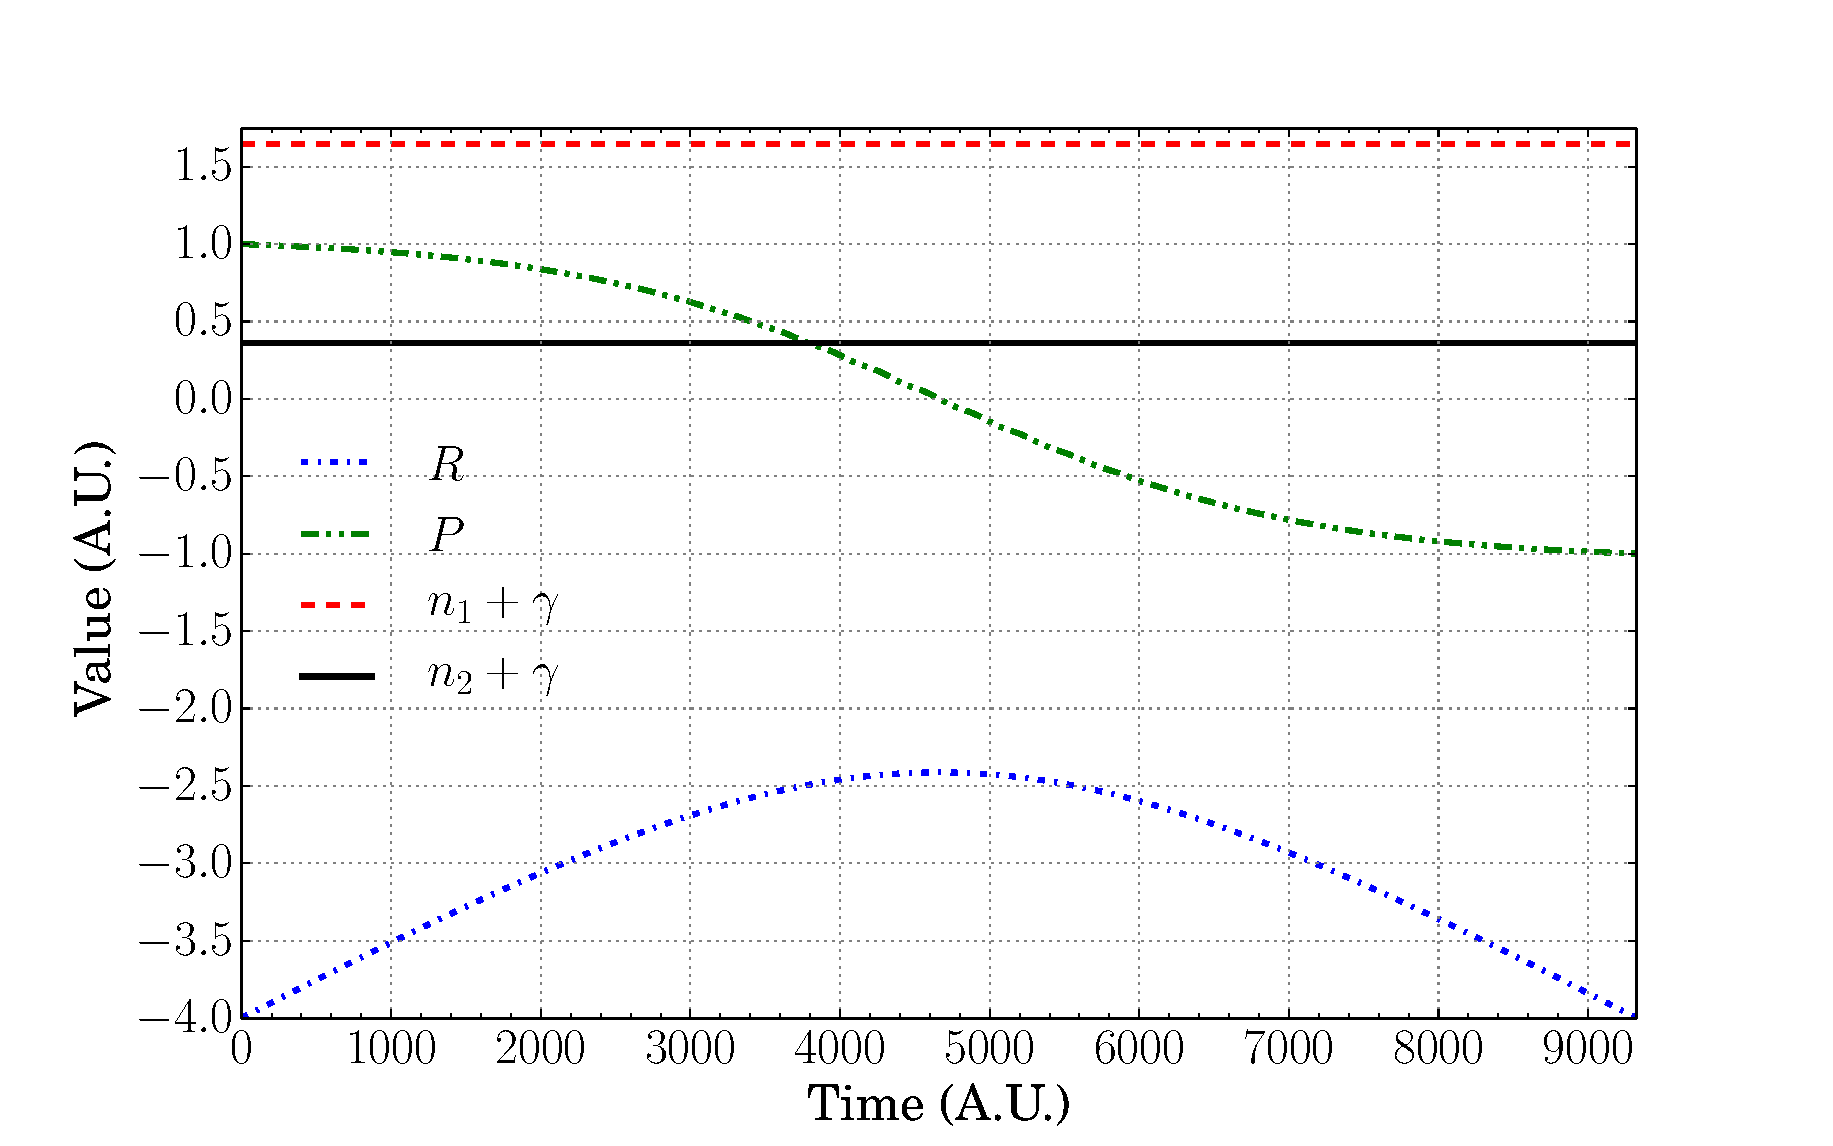
\includegraphics[width=\textwidth]{sc_traj_r11.eps}
\vspace{-0.1cm}
\caption{{\fontsize{7}{8}\selectfont \roo.}}
\end{subfigure}
~
\begin{subfigure}[t]{0.45\textwidth}
\centering
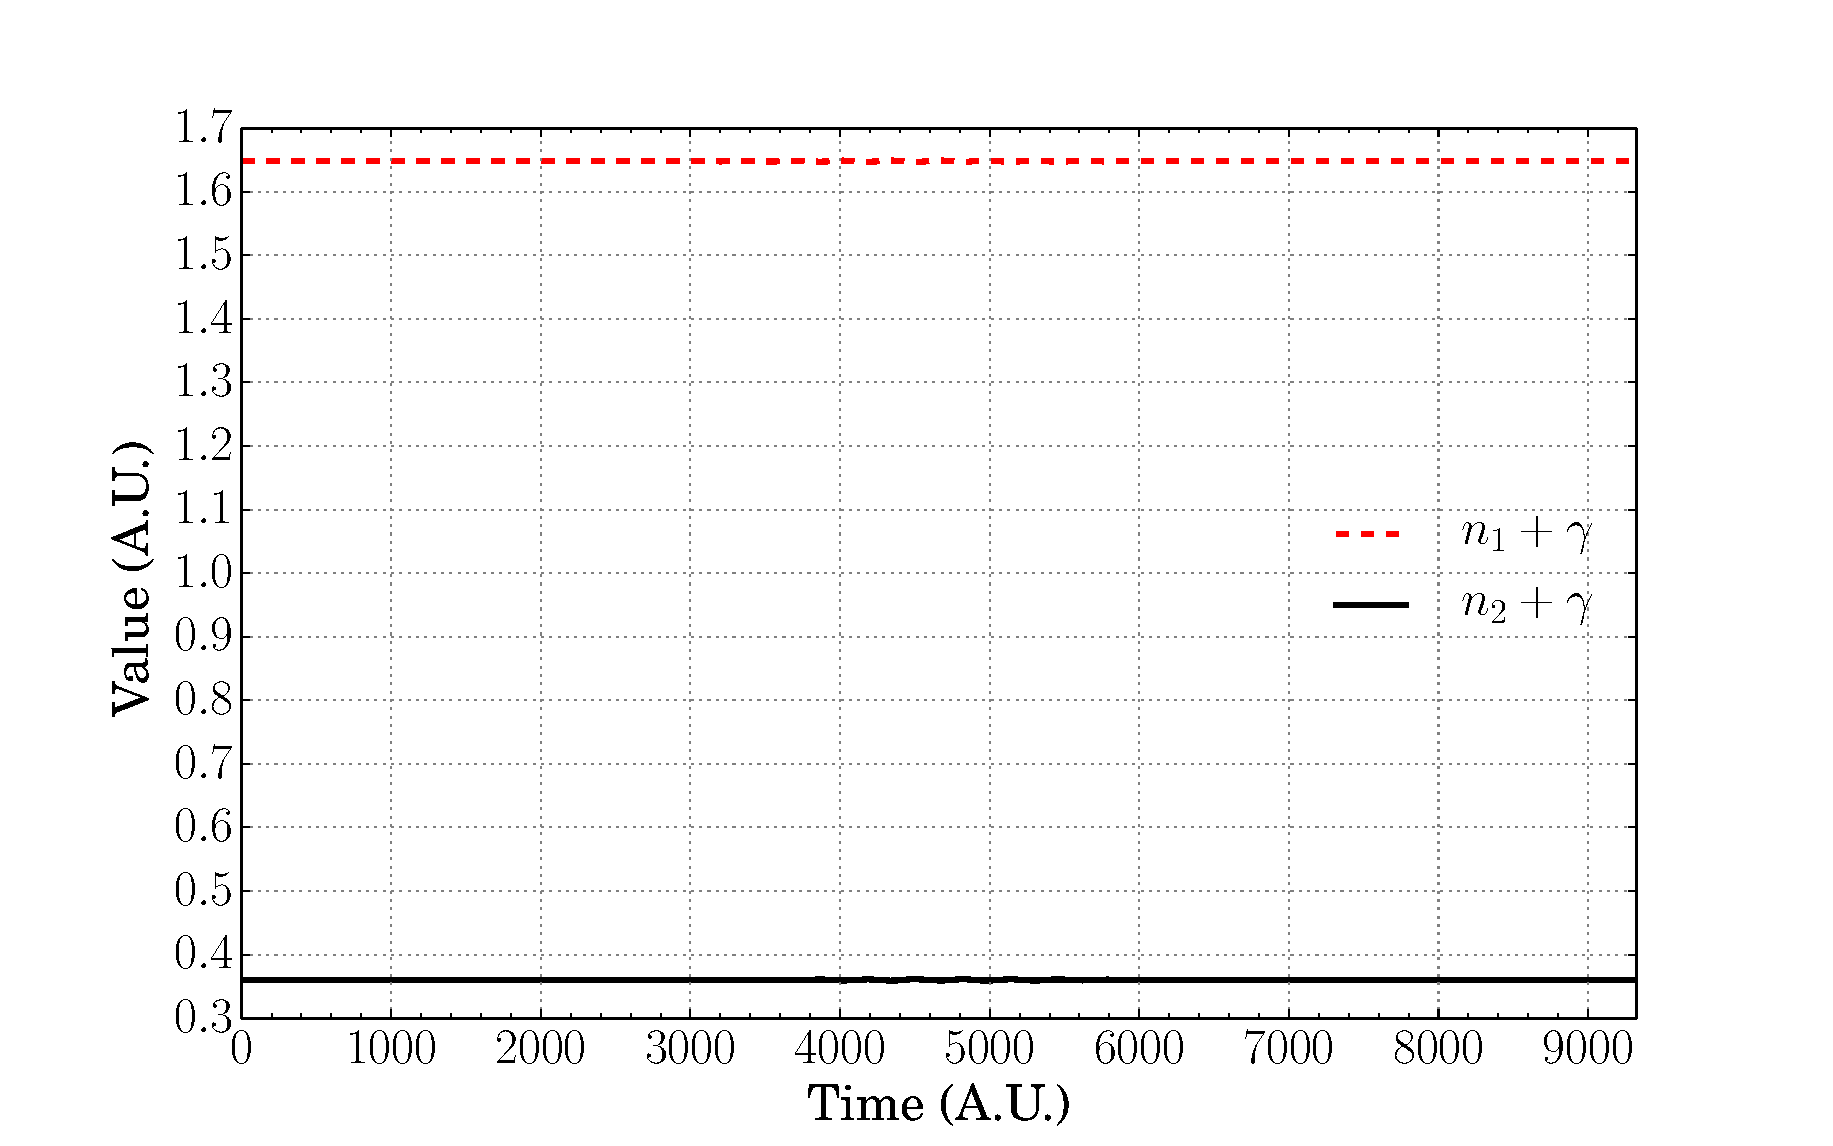
\includegraphics[width=\textwidth]{sc_traj_r11_e.eps}
\vspace{-0.1cm}
\caption{{\fontsize{7}{8}\selectfont \roo, zoom into $ n_{1}$, $n_{2} $.}}
\end{subfigure}
\\[-0.32cm]
\begin{subfigure}[t]{0.45\textwidth}
\centering
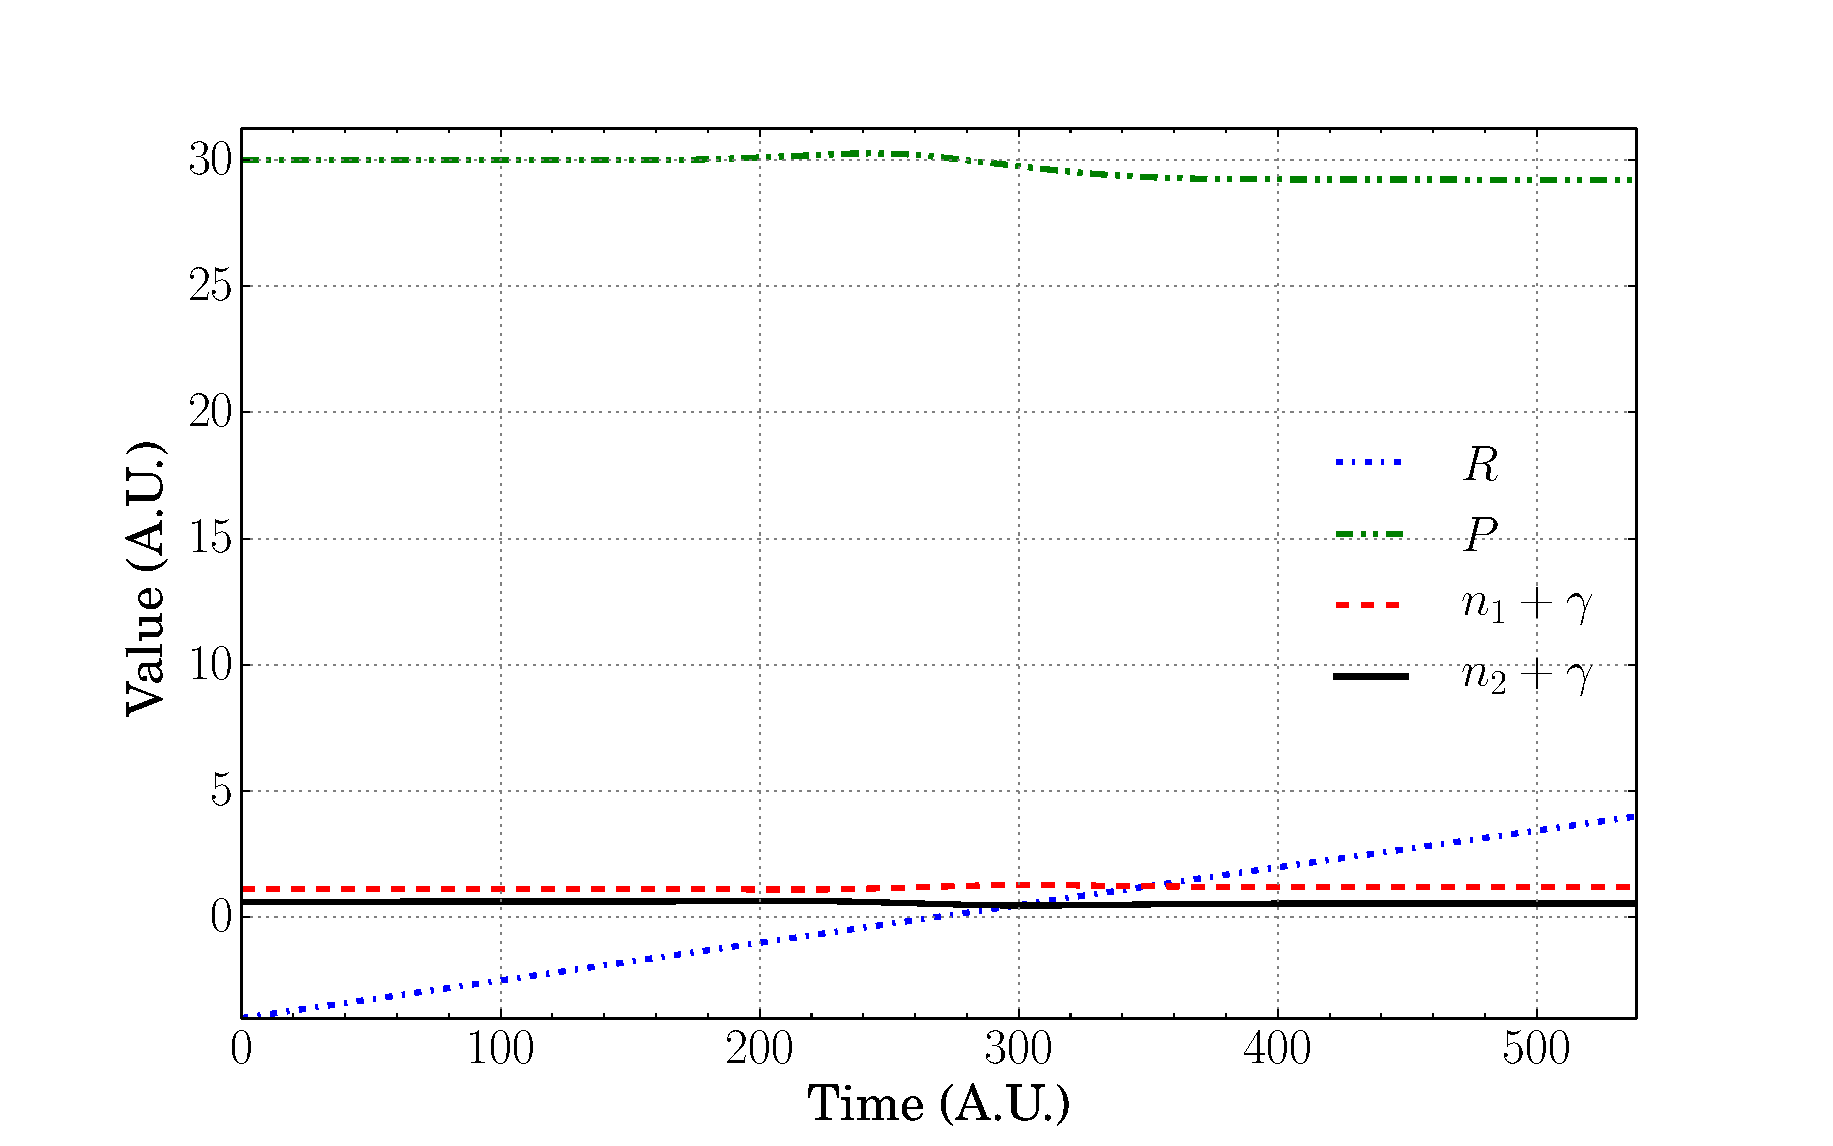
\includegraphics[width=\textwidth]{sc_traj_t11.eps}
\vspace{-0.1cm}
\caption{{\fontsize{7}{8}\selectfont \too.}}
\end{subfigure}
~
\begin{subfigure}[t]{0.45\textwidth}
\centering
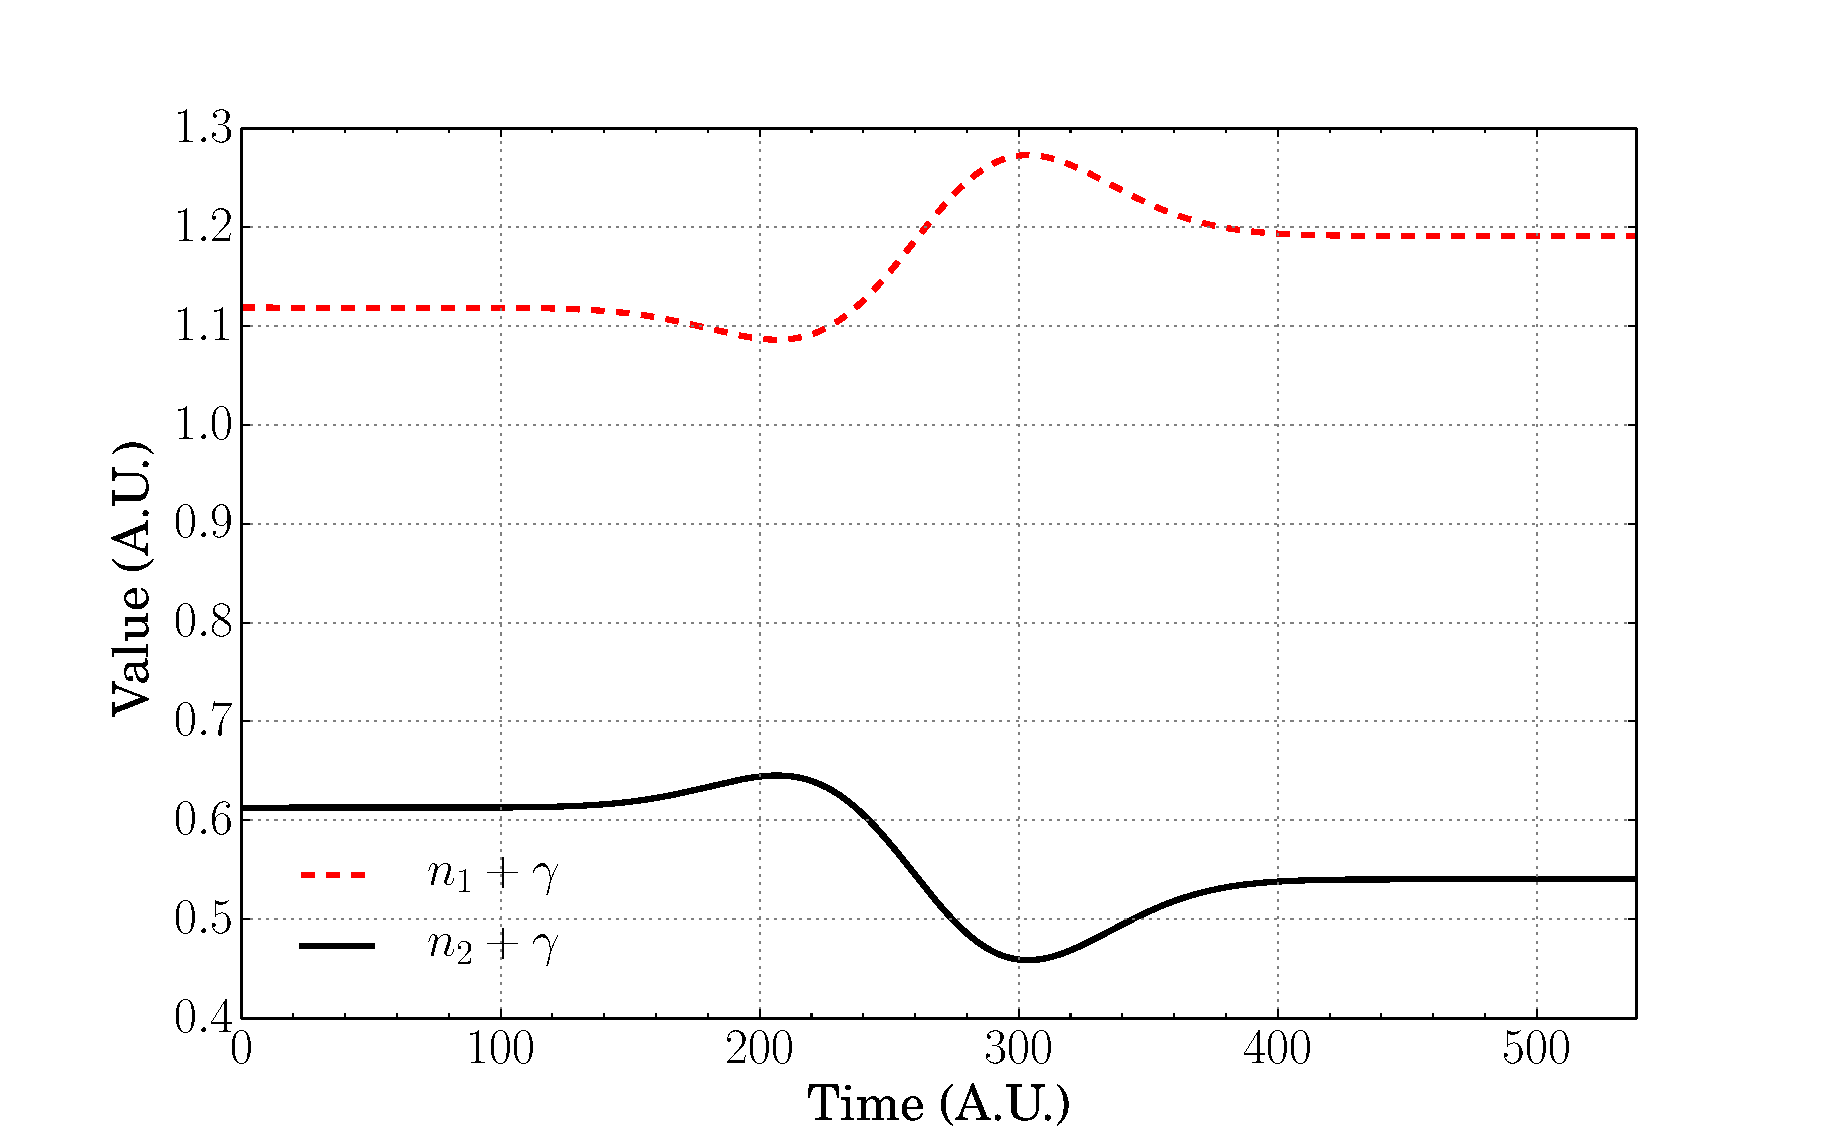
\includegraphics[width=\textwidth]{sc_traj_t11_e.eps}
\vspace{-0.1cm}
\caption{{\fontsize{7}{8}\selectfont \too, zoom into $ n_{1}$, $n_{2} $.}}
\end{subfigure}
\vspace{-0.1cm}
\caption{$ i = 1 $, sample trajectories.}
\end{figure}
}{\stepcounter{figure}}

\alt<4>{
\framesubtitle{Sample Trajectories ($ i=1 $).}
\begin{figure}
\begin{subfigure}[t]{0.48\textwidth}
\centering
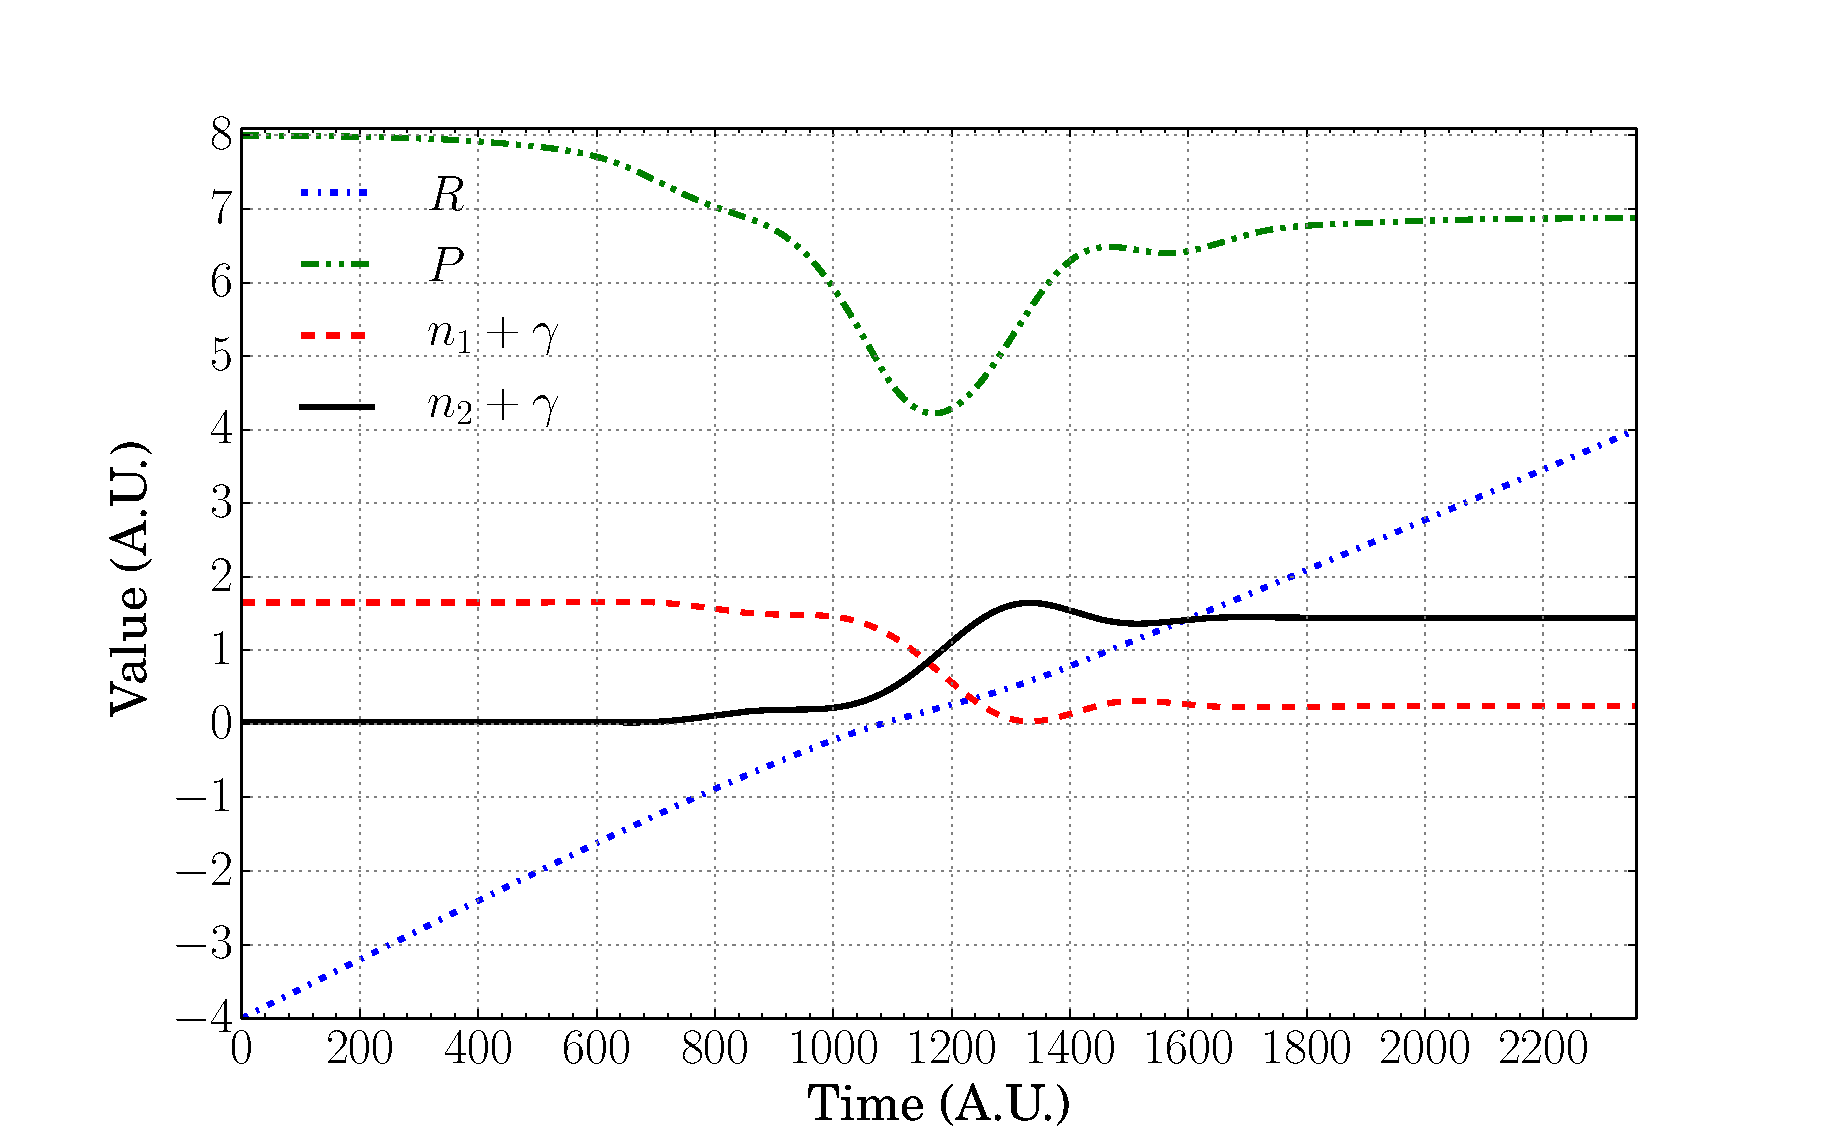
\includegraphics[width=\textwidth]{sc_traj_t21.eps}
\caption{\tto.}
\end{subfigure}
~
\begin{subfigure}[t]{0.48\textwidth}
\centering
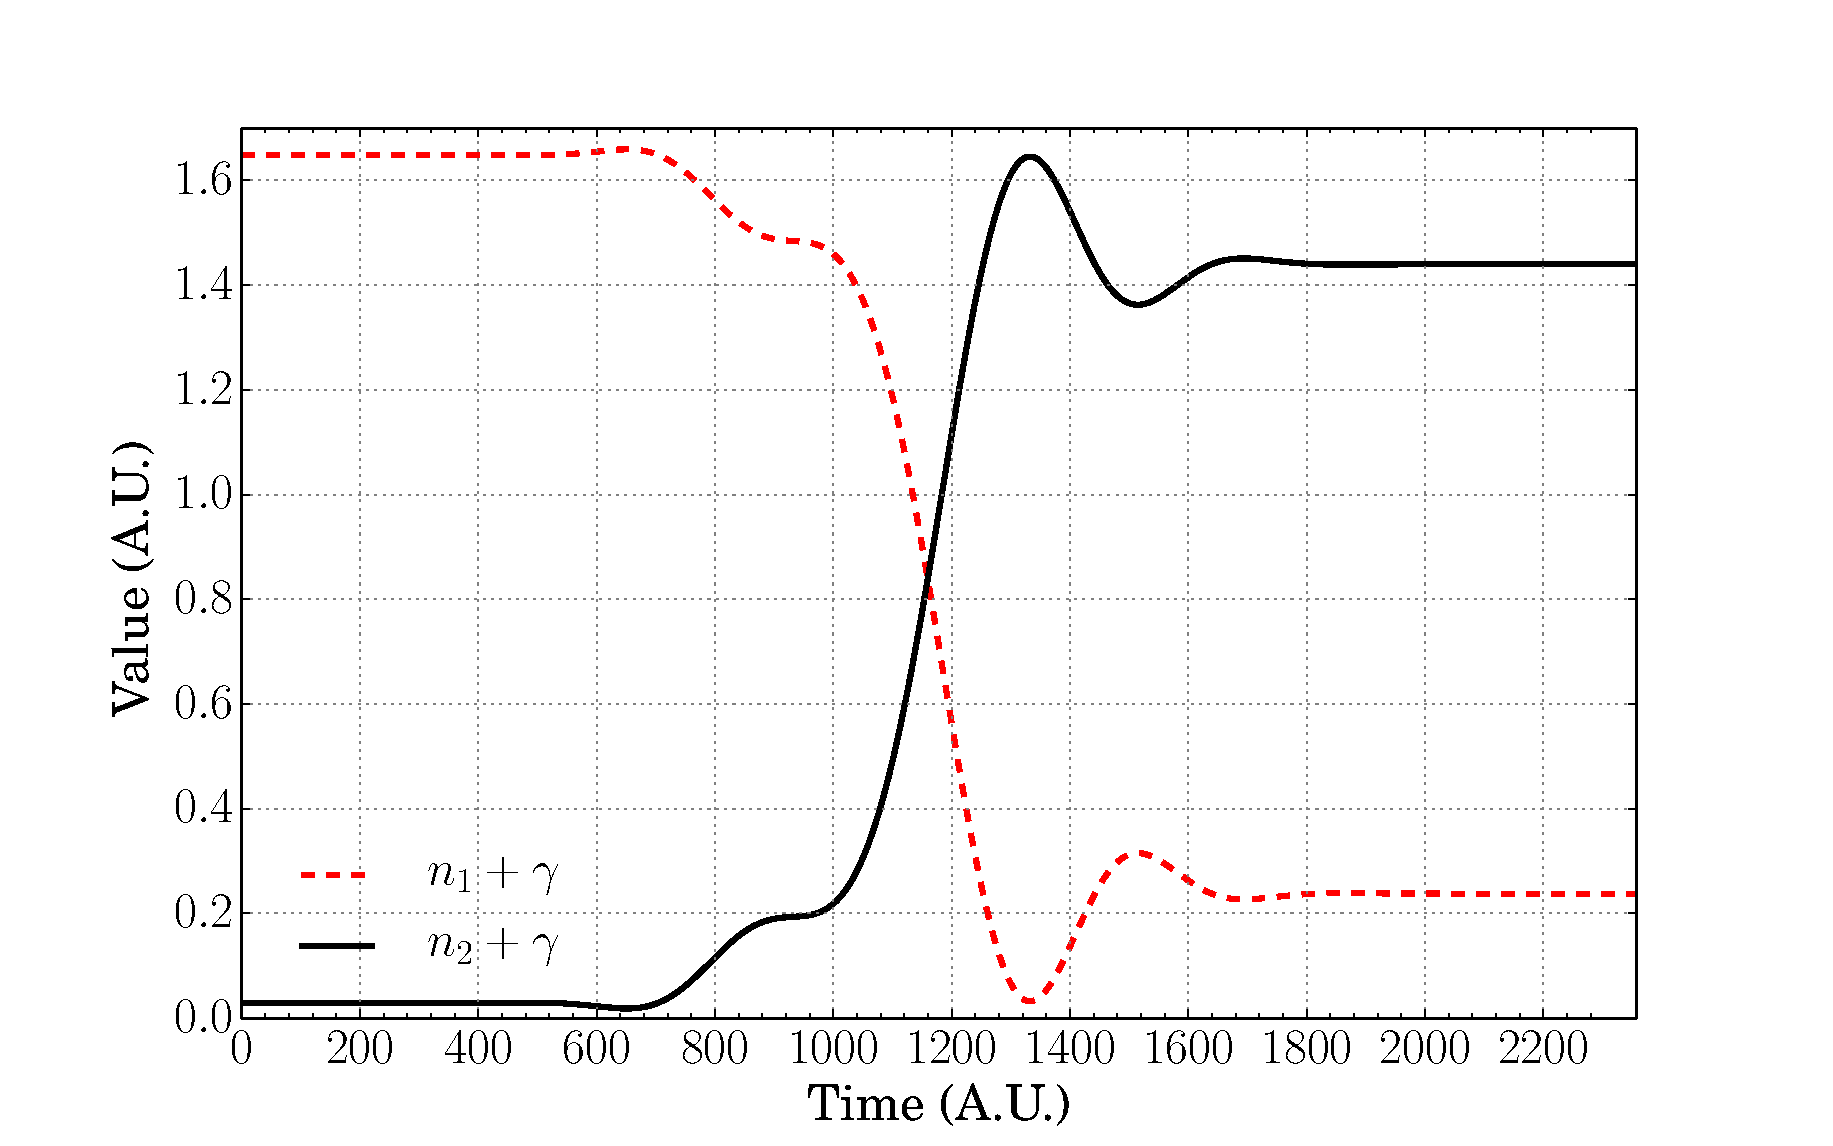
\includegraphics[width=\textwidth]{sc_traj_t21_e.eps}
\caption{\tto, zoom into $ n_{1}$, $n_{2} $.}
\end{subfigure}
\caption{$ i = 1 $, sample trajectories.}
\end{figure}
}{\stepcounter{figure}}

\alt<5>{
\framesubtitle{Sample Trajectories ($ i=2 $).}
\vspace{-0.3cm}
\begin{figure}
\begin{subfigure}[t]{0.45\textwidth}
\centering
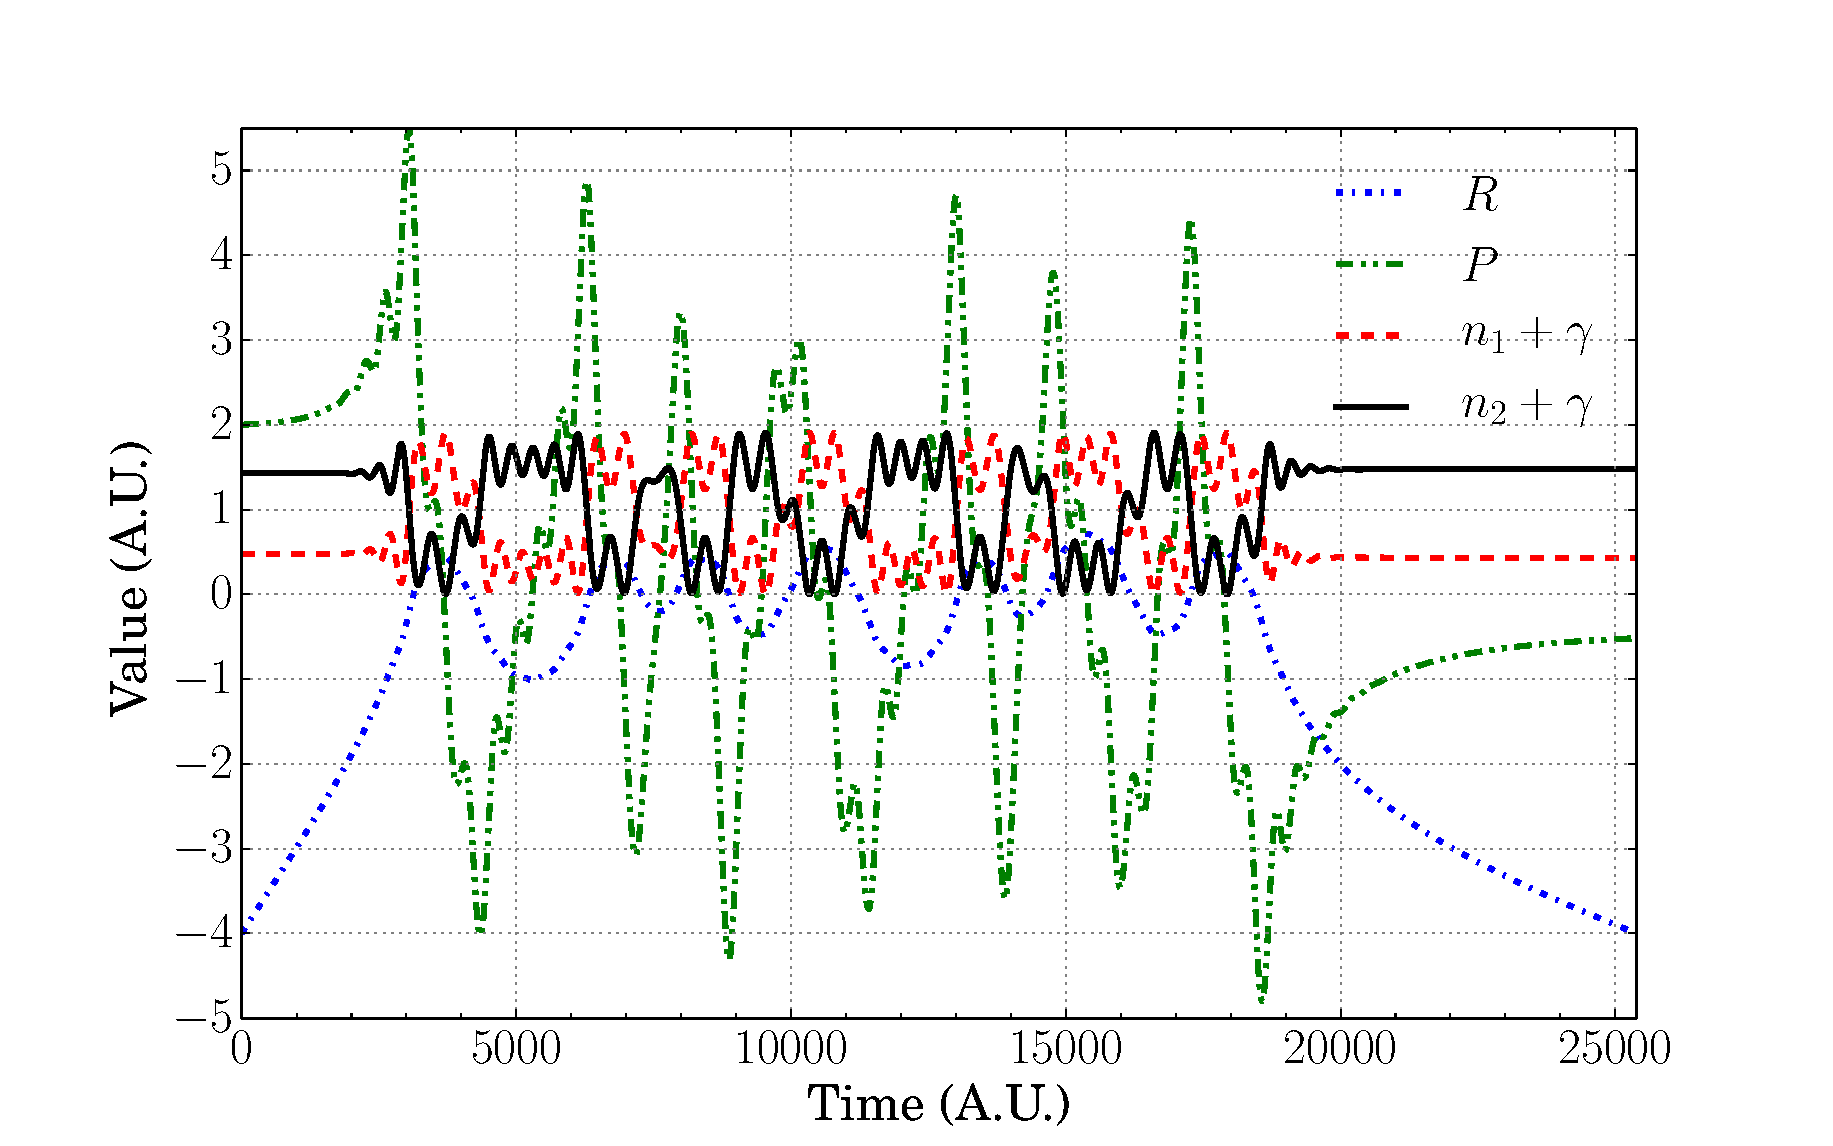
\includegraphics[width=\textwidth]{sc_traj_r22.eps}
\vspace{-0.1cm}
\caption{{\fontsize{7}{8}\selectfont \rtt.}}
\end{subfigure}
~
\begin{subfigure}[t]{0.45\textwidth}
\centering
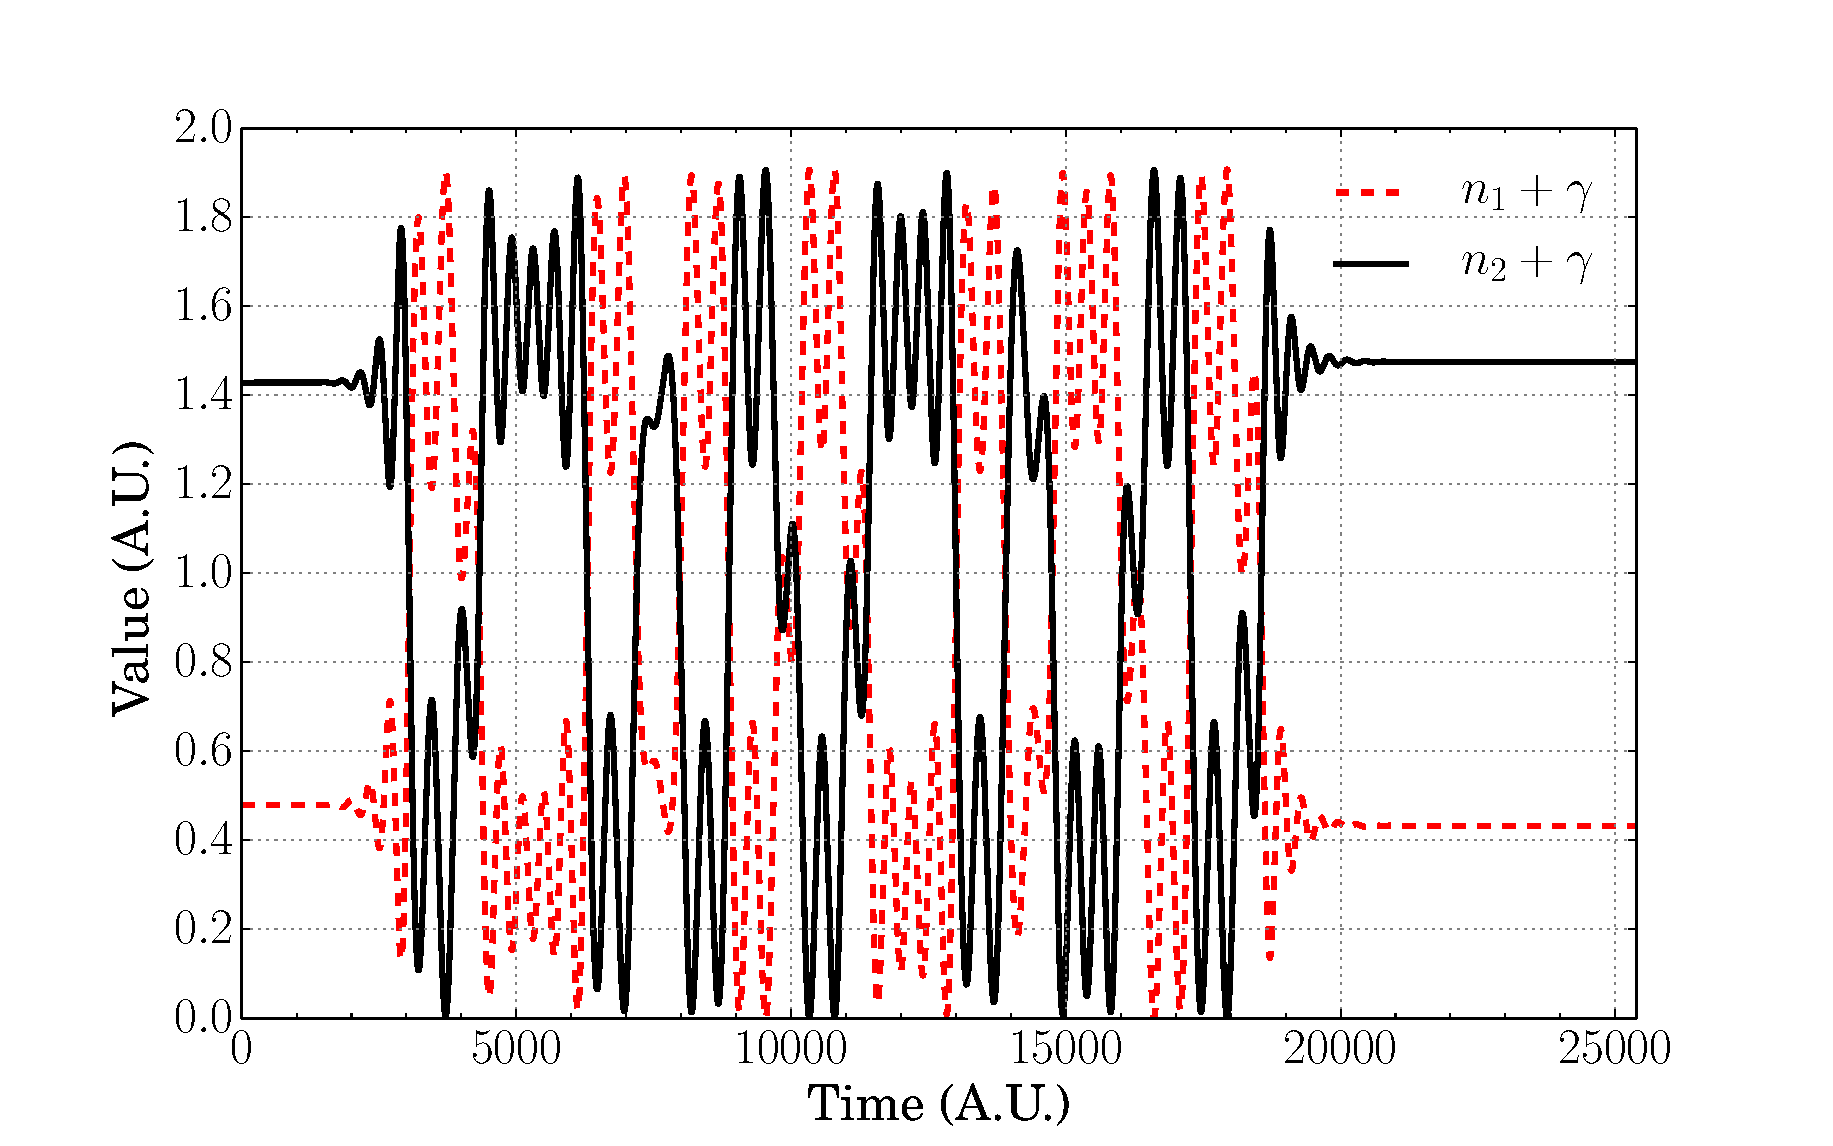
\includegraphics[width=\textwidth]{sc_traj_r22_e.eps}
\vspace{-0.1cm}
\caption{{\fontsize{7}{8}\selectfont \rtt, zoom into $ n_{1} $, $ n_{2} $.}}
\end{subfigure}
\\[-0.32cm]
\begin{subfigure}[t]{0.45\textwidth}
\centering
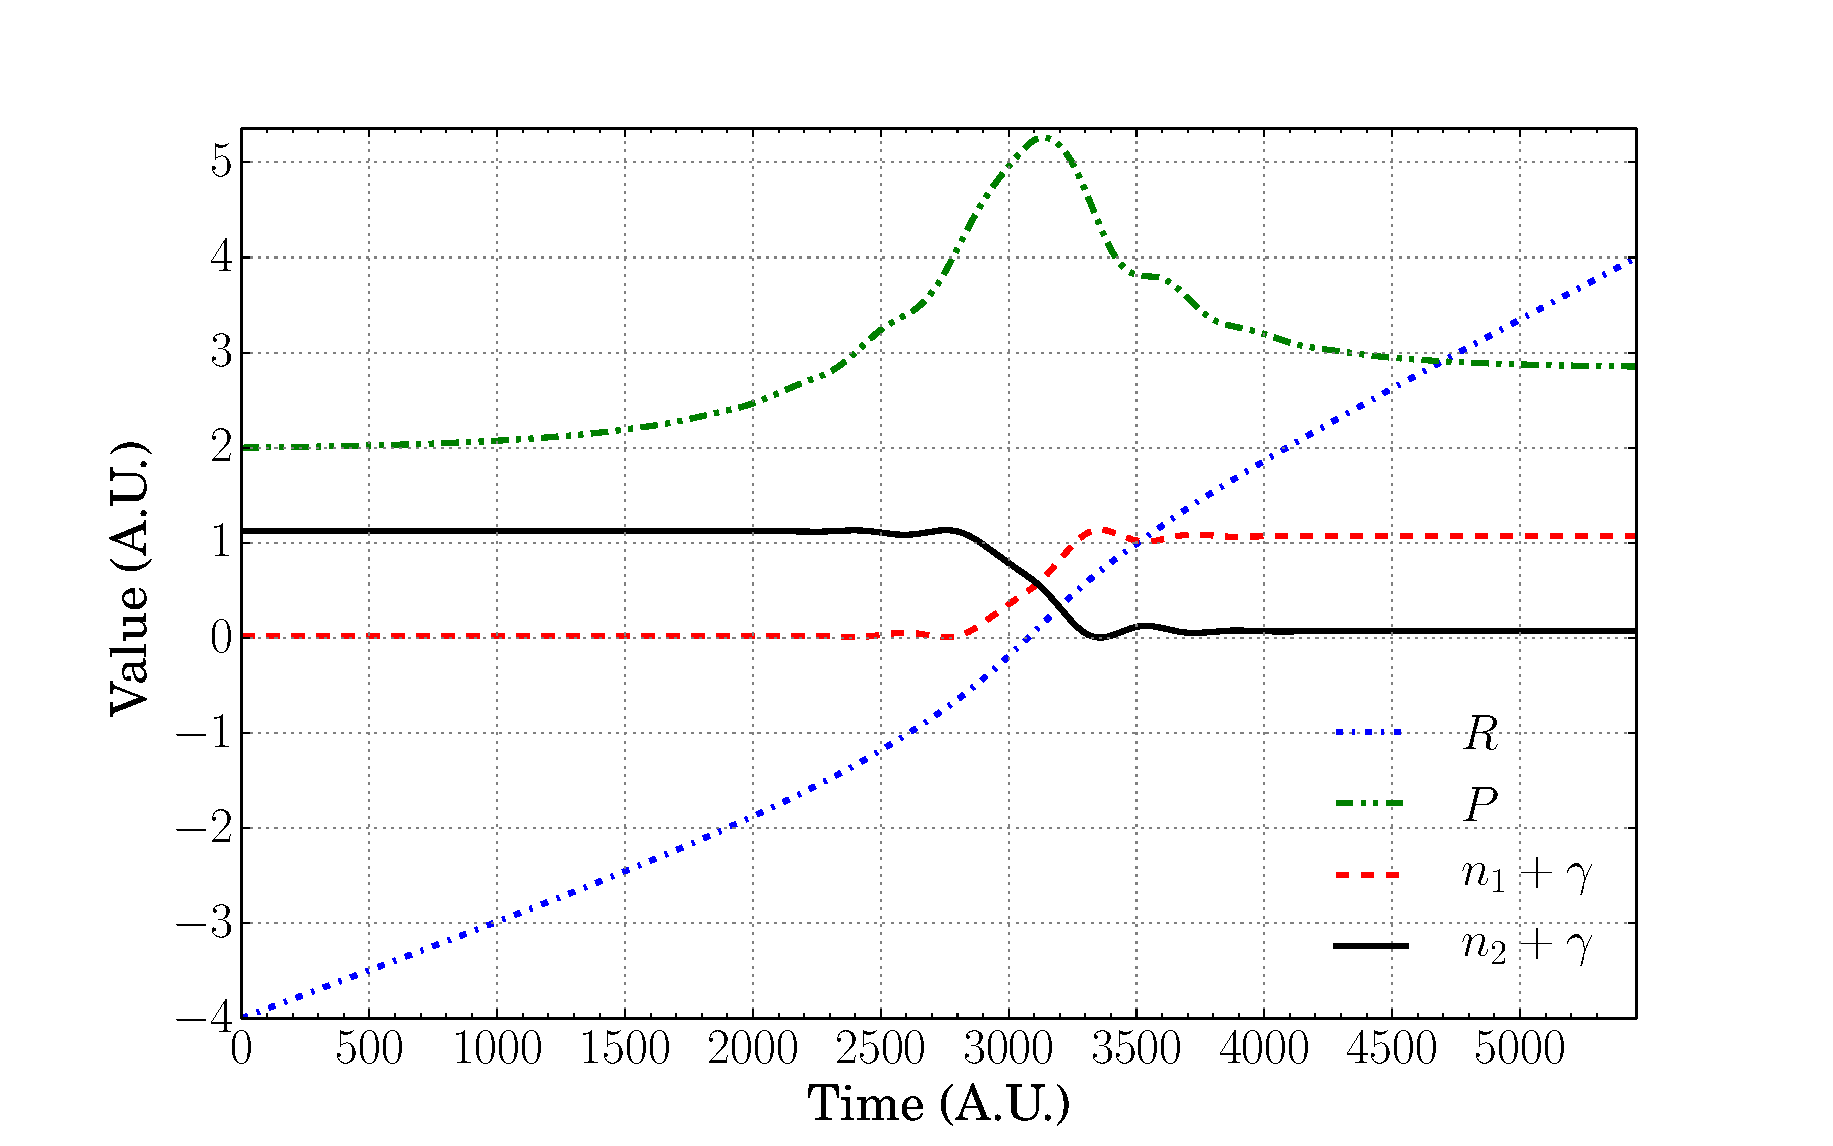
\includegraphics[width=\textwidth]{sc_traj_t12.eps}
\vspace{-0.1cm}
\caption{{\fontsize{7}{8}\selectfont \tot.}}
\end{subfigure}
~
\begin{subfigure}[t]{0.45\textwidth}
\centering
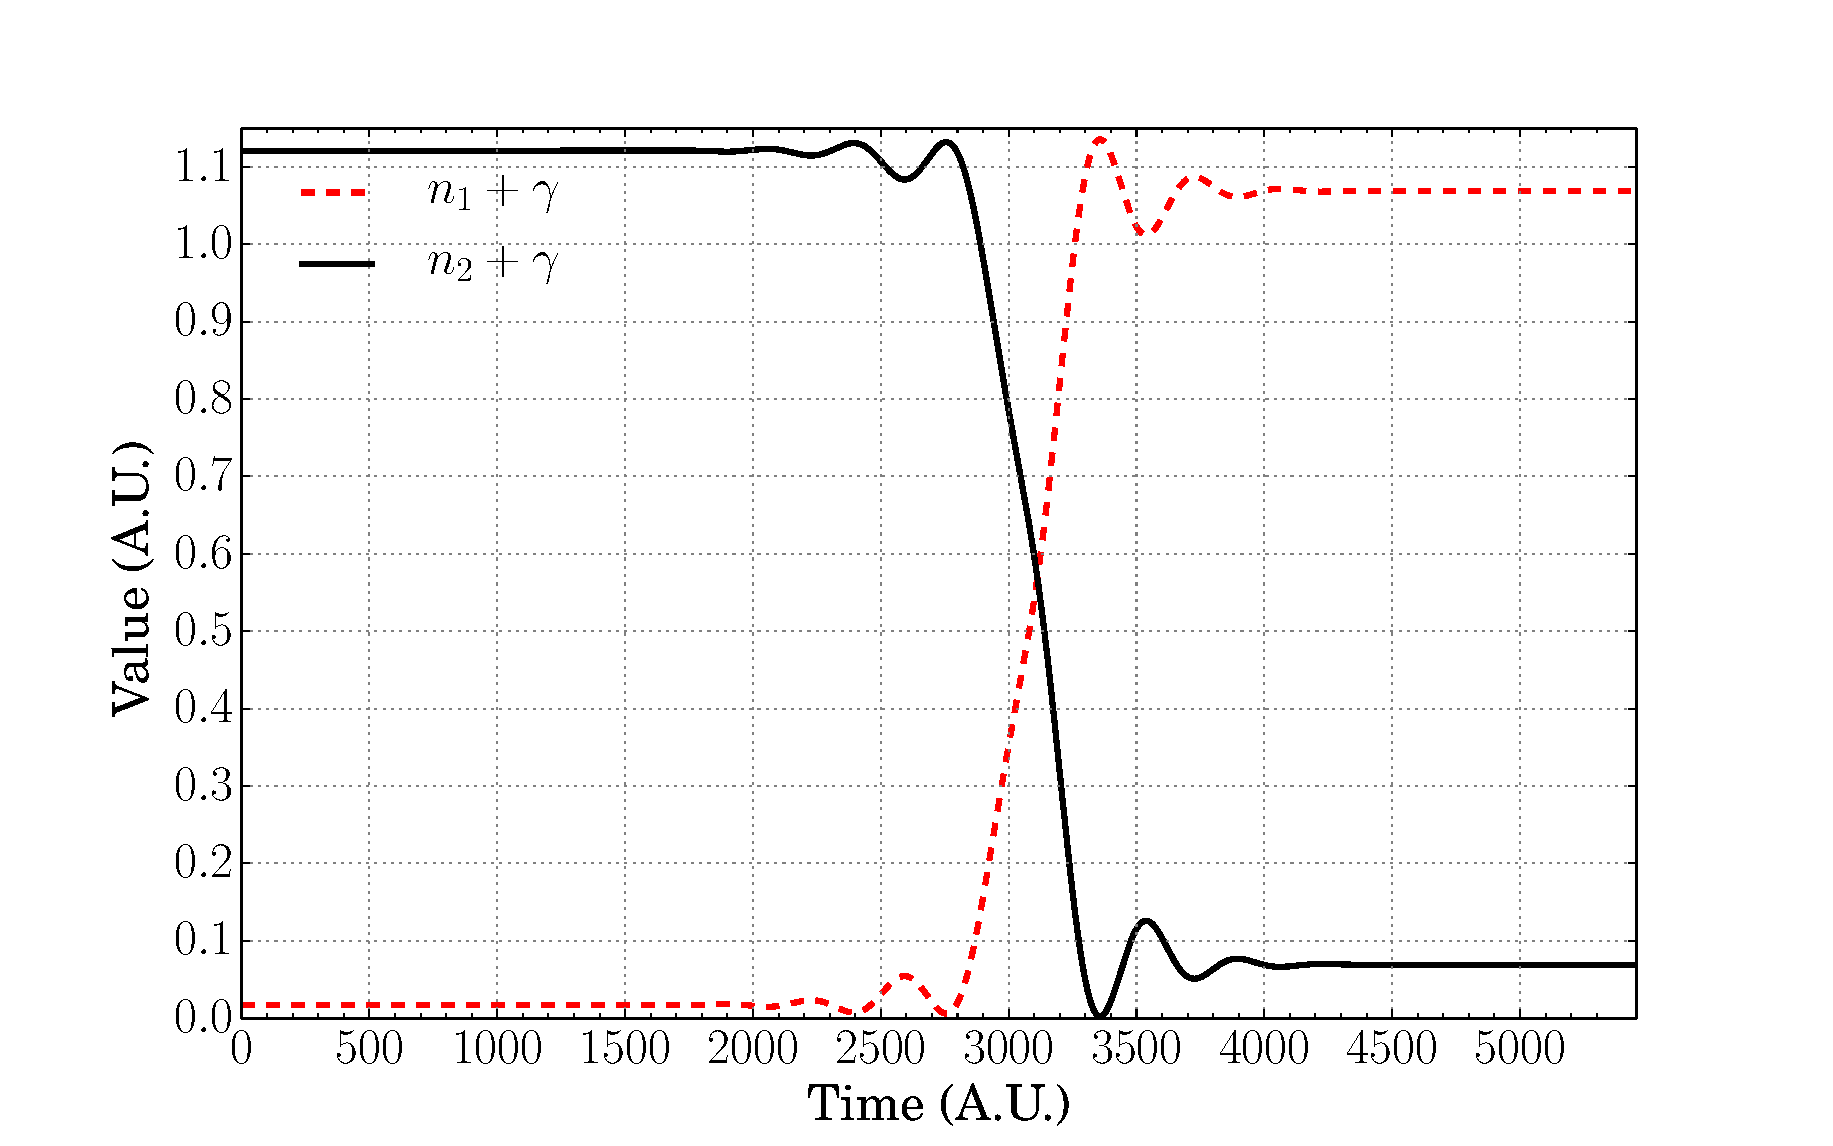
\includegraphics[width=\textwidth]{sc_traj_t12_e.eps}
\vspace{-0.1cm}
\caption{{\fontsize{7}{8}\selectfont \tot, zoom into $ n_{1}$, $n_{2} $.}}
\end{subfigure}
\caption{$ i = 2 $, sample trajectories.}
\end{figure}
}{\stepcounter{figure}}

\alt<6>{
\framesubtitle{Sample Trajectories ($ i=2 $).}
\begin{figure}
\begin{subfigure}[t]{0.48\textwidth}
\centering
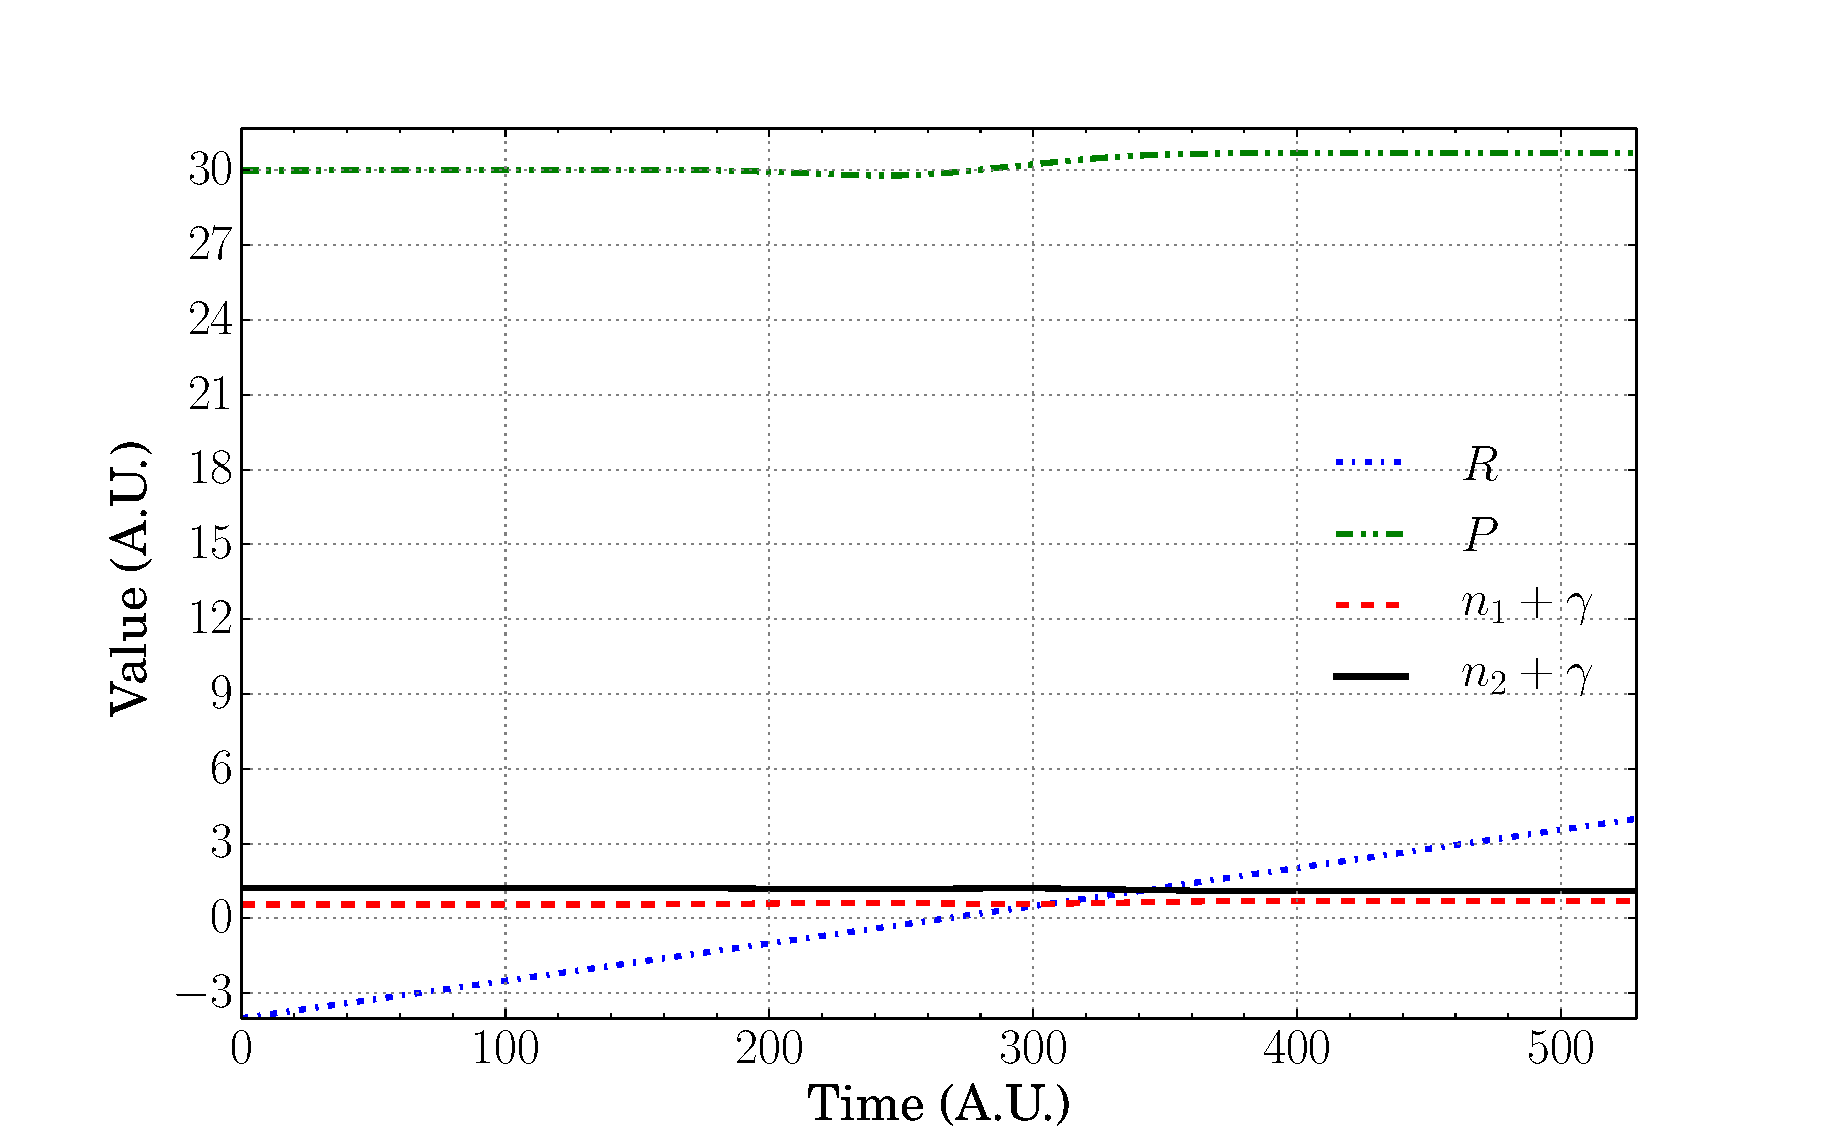
\includegraphics[width=\textwidth]{sc_traj_t22.eps}
\caption{\ttt.}
\end{subfigure}
~
\begin{subfigure}[t]{0.48\textwidth}
\centering
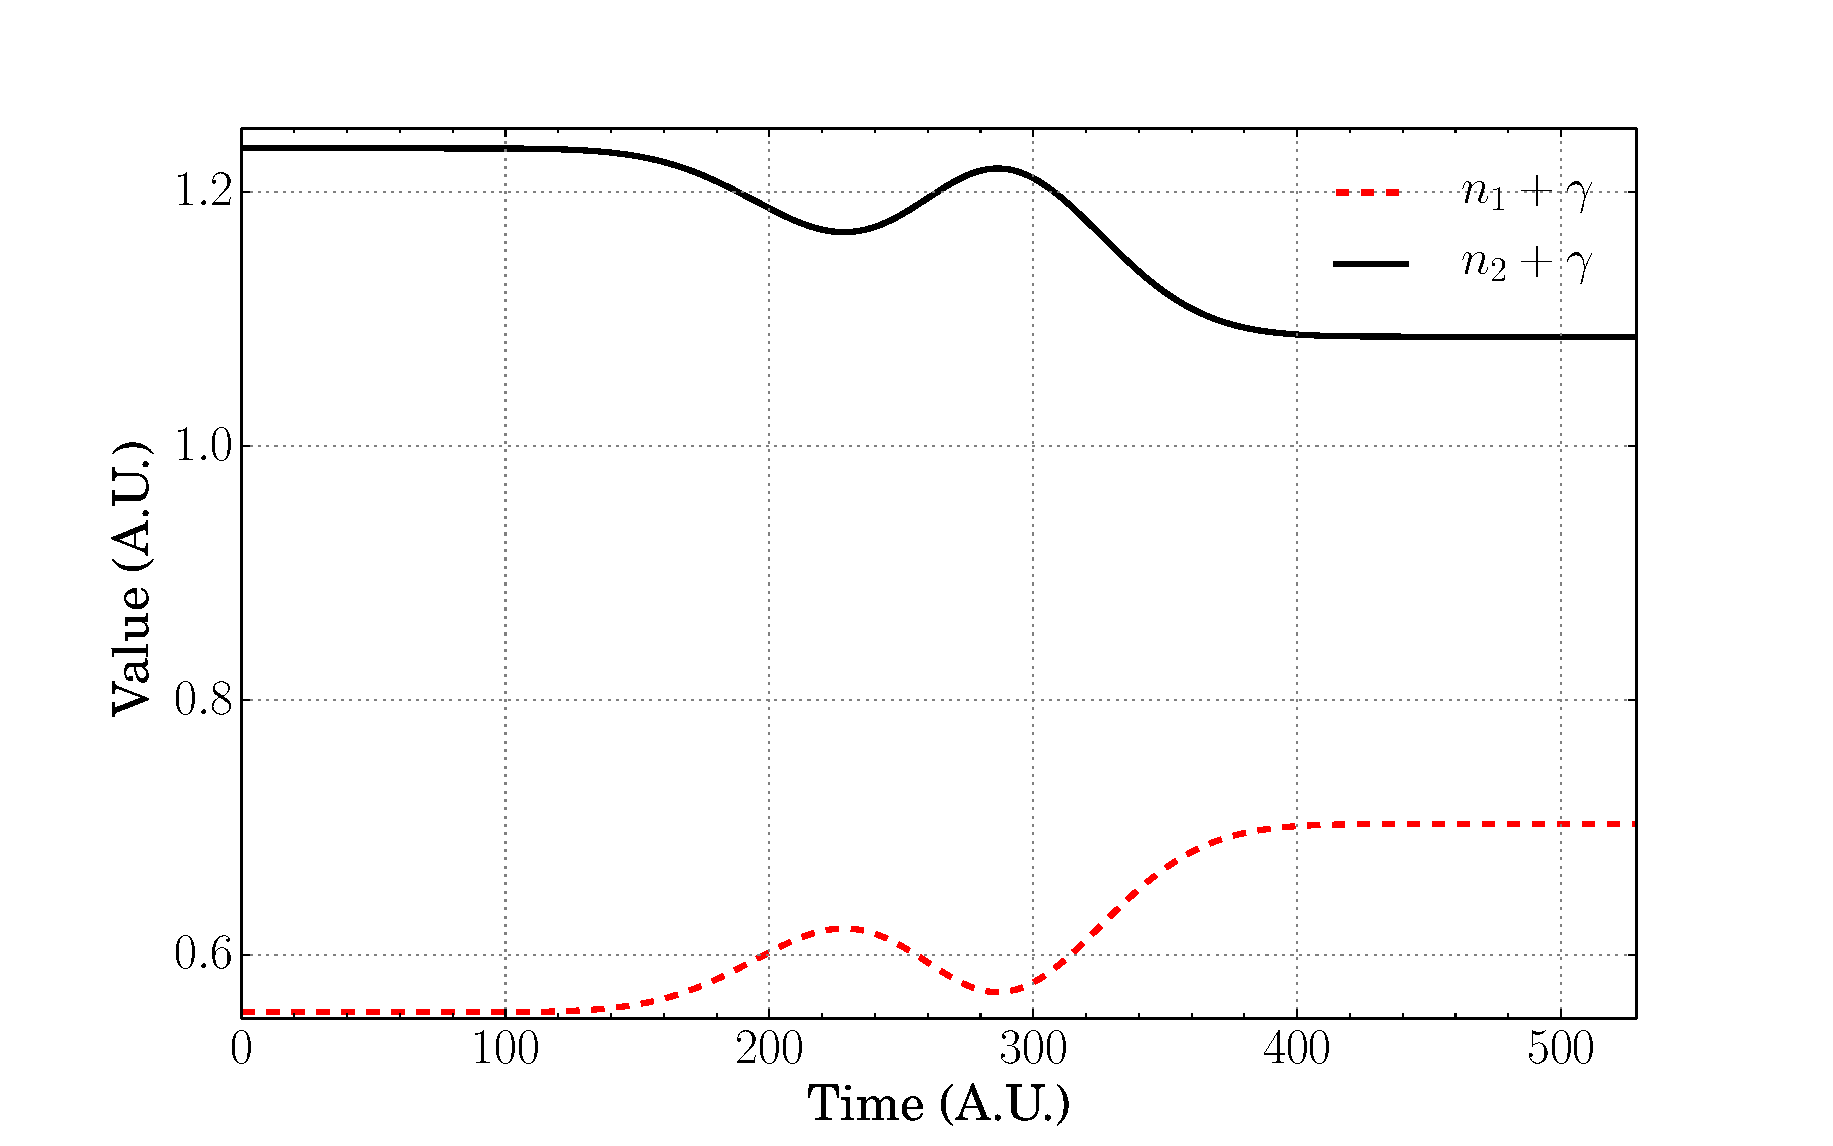
\includegraphics[width=\textwidth]{sc_traj_t22_e.eps}
\caption{\ttt, zoom a $ n_{1}$, $n_{2} $.}
\end{subfigure}
\caption{$ i = 2 $, sample trajectories.}
\end{figure}
}{\stepcounter{figure}}
\end{frame}

\subsection{Double Avoided Crossing}
\begin{frame}
\frametitle{Double Avoided Crossing}
\alt<1>{
\framesubtitle{Diabatic PES Derivatives (DPES)}
\begin{subequations}
\begin{align}
\dpar{H_{11}}{R} &= 0\\
\dpar{H_{22}}{R} &= 2 A B e^{-B R^{2}} R\\
\dpar{H_{12}}{R} &= \dpar{H_{21}}{R} = -2 C D e^{-D R^{2}} R
\end{align}
\end{subequations}
}{\stepcounter{equation}}

\alt<2>{
\framesubtitle{Adiabatic PES (APES)}
\begin{subequations}
\begin{align}
E_{1} &= \frac{1}{2} e^{-(B+D) R^{2}}
\left(
\begin{aligned}
&-A e^{D R^{2}} + e^{(B+D) R^{2}} E_{0} \\
&-\sqrt{
4 C^{2} e^{2 B R^{2}} + e^{2 D R^{2}}\left( A - e^{B R^{2}} E_{0} \right)^{2}
}
\end{aligned}\right)\\
E_{2} &= \frac{1}{2} e^{-(B+D) R^{2}}
\left(
\begin{aligned}
&-A e^{D R^{2}} + e^{(B+D) R^{2}} E_{0} \\
&+\sqrt{
4 C^{2} e^{2 B R^{2}} + e^{2 D R^{2}}\left( A - e^{B R^{2}} E_{0} \right)^{2}
}
\end{aligned}\right)
\end{align}
\end{subequations}
}{\stepcounter{equation}}

\alt<3>{
\framesubtitle{Sample Trajectories ($ i=1 $).}
\vspace{-0.3cm}
\begin{figure}
\centering
\begin{subfigure}[t]{0.45\textwidth}
\centering
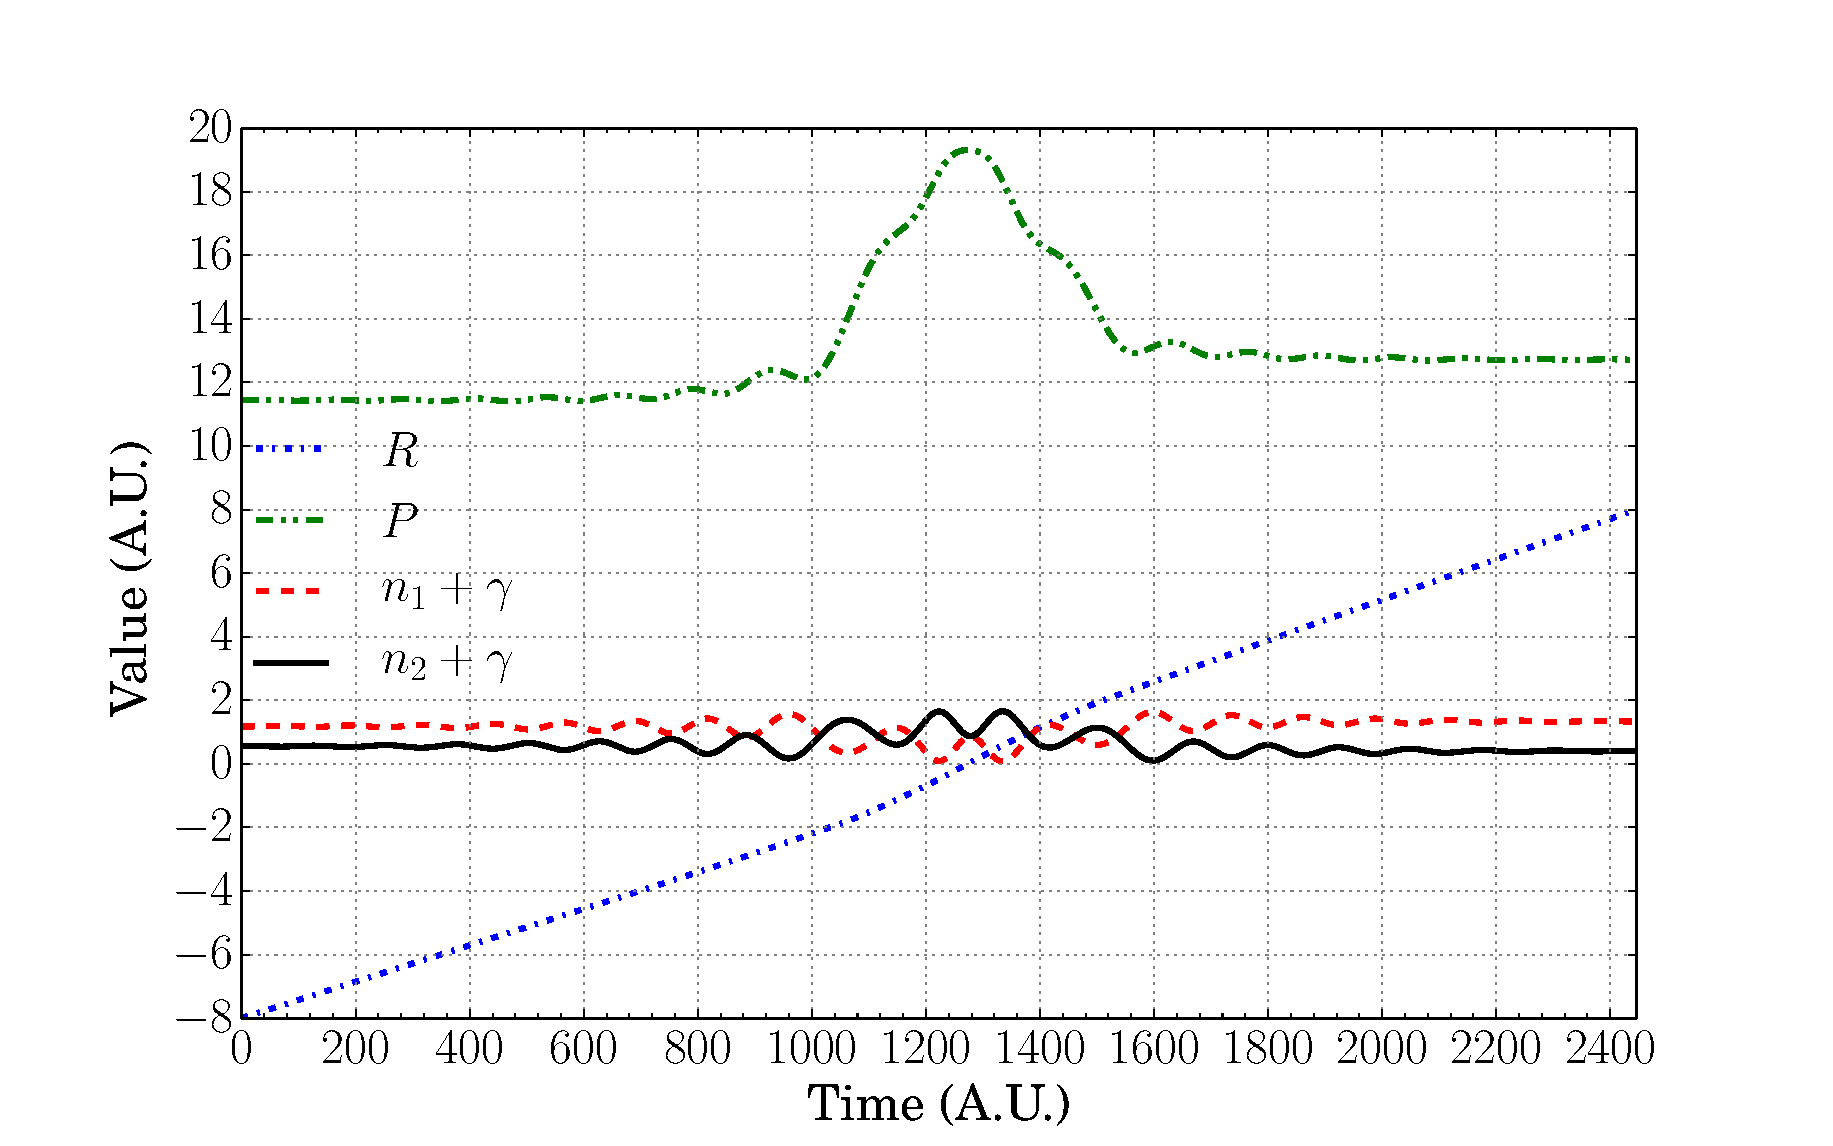
\includegraphics[width=\textwidth]{dc_traj_t11.eps}
\vspace{-0.1cm}
\caption{{\fontsize{7}{8}\selectfont \too.}}
\end{subfigure}
~
\begin{subfigure}[t]{0.45\textwidth}
\centering
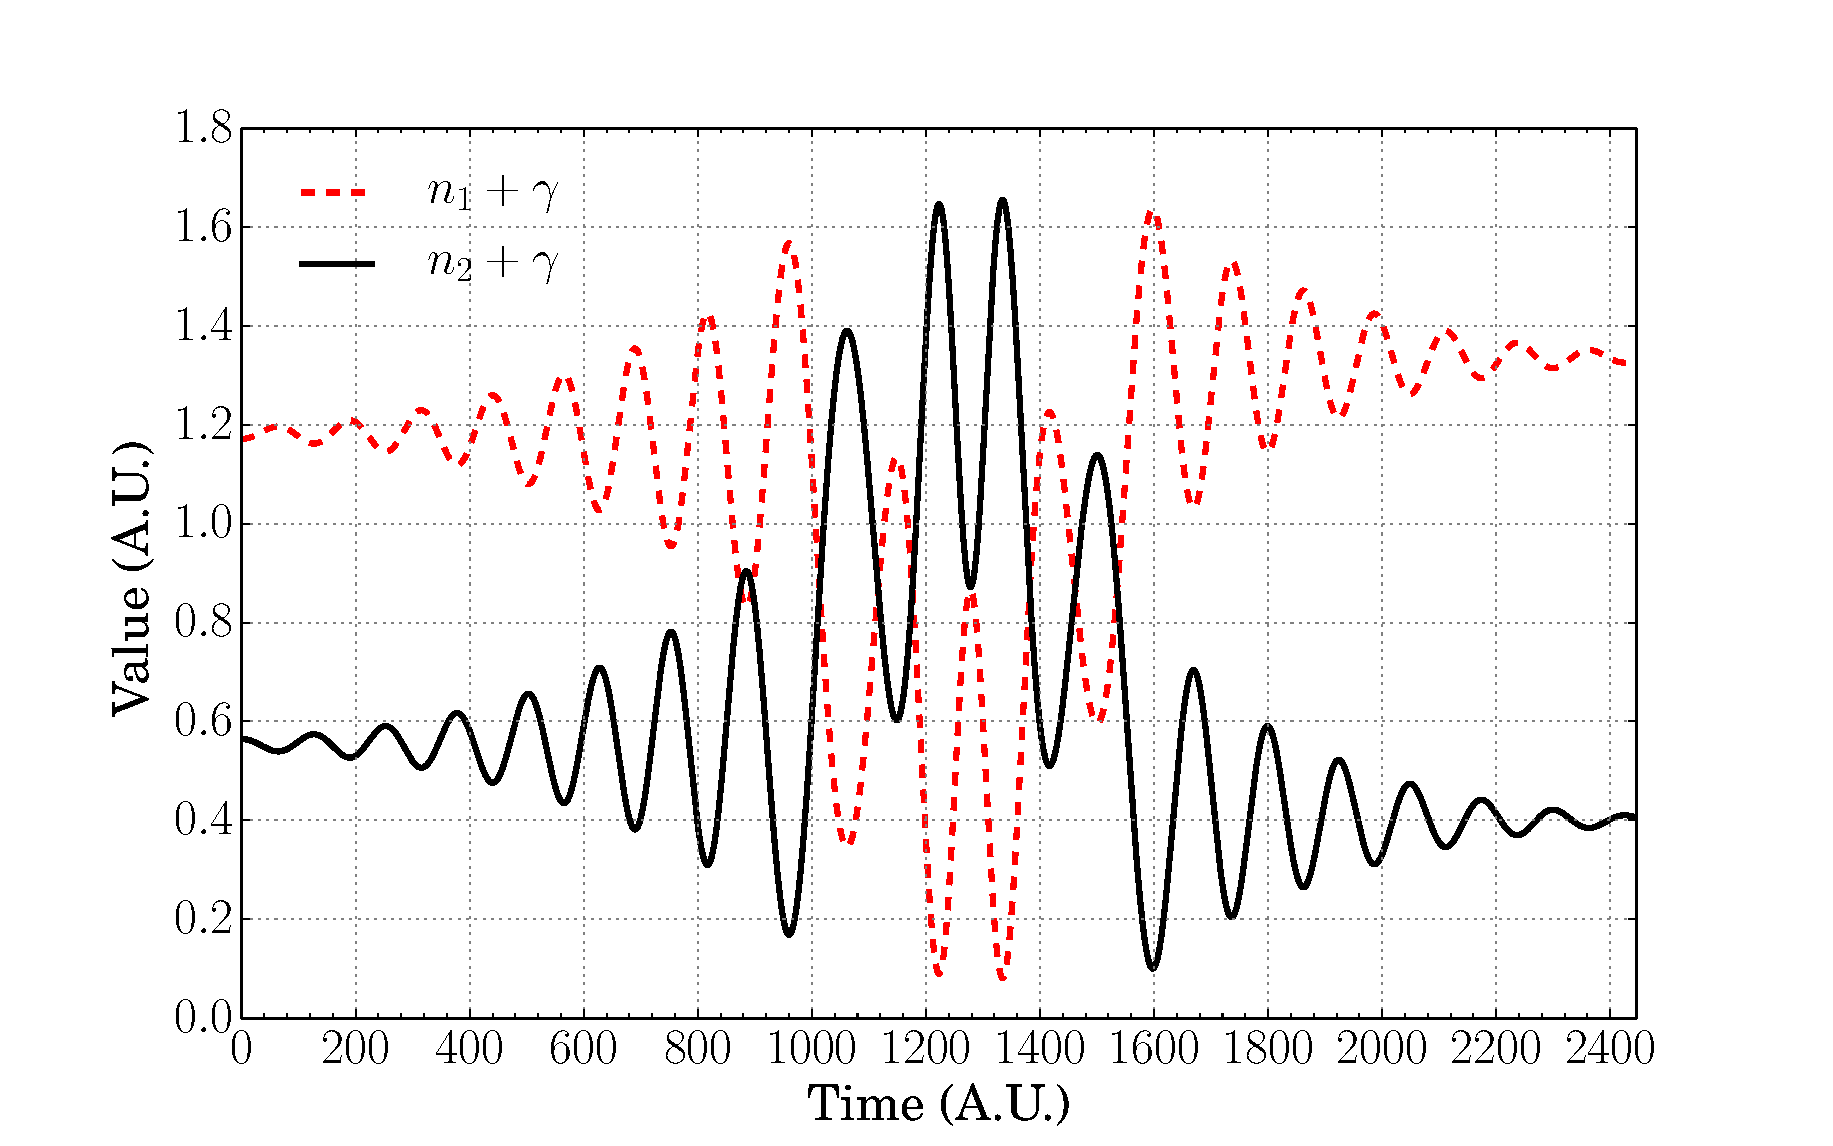
\includegraphics[width=\textwidth]{dc_traj_t11_e.eps}
\vspace{-0.1cm}
\caption{{\fontsize{7}{8}\selectfont \too, zoom into $ n_{1}$, $n_{2} $.}}
\end{subfigure}
\\[-0.32cm]
\begin{subfigure}[t]{0.45\textwidth}
\centering
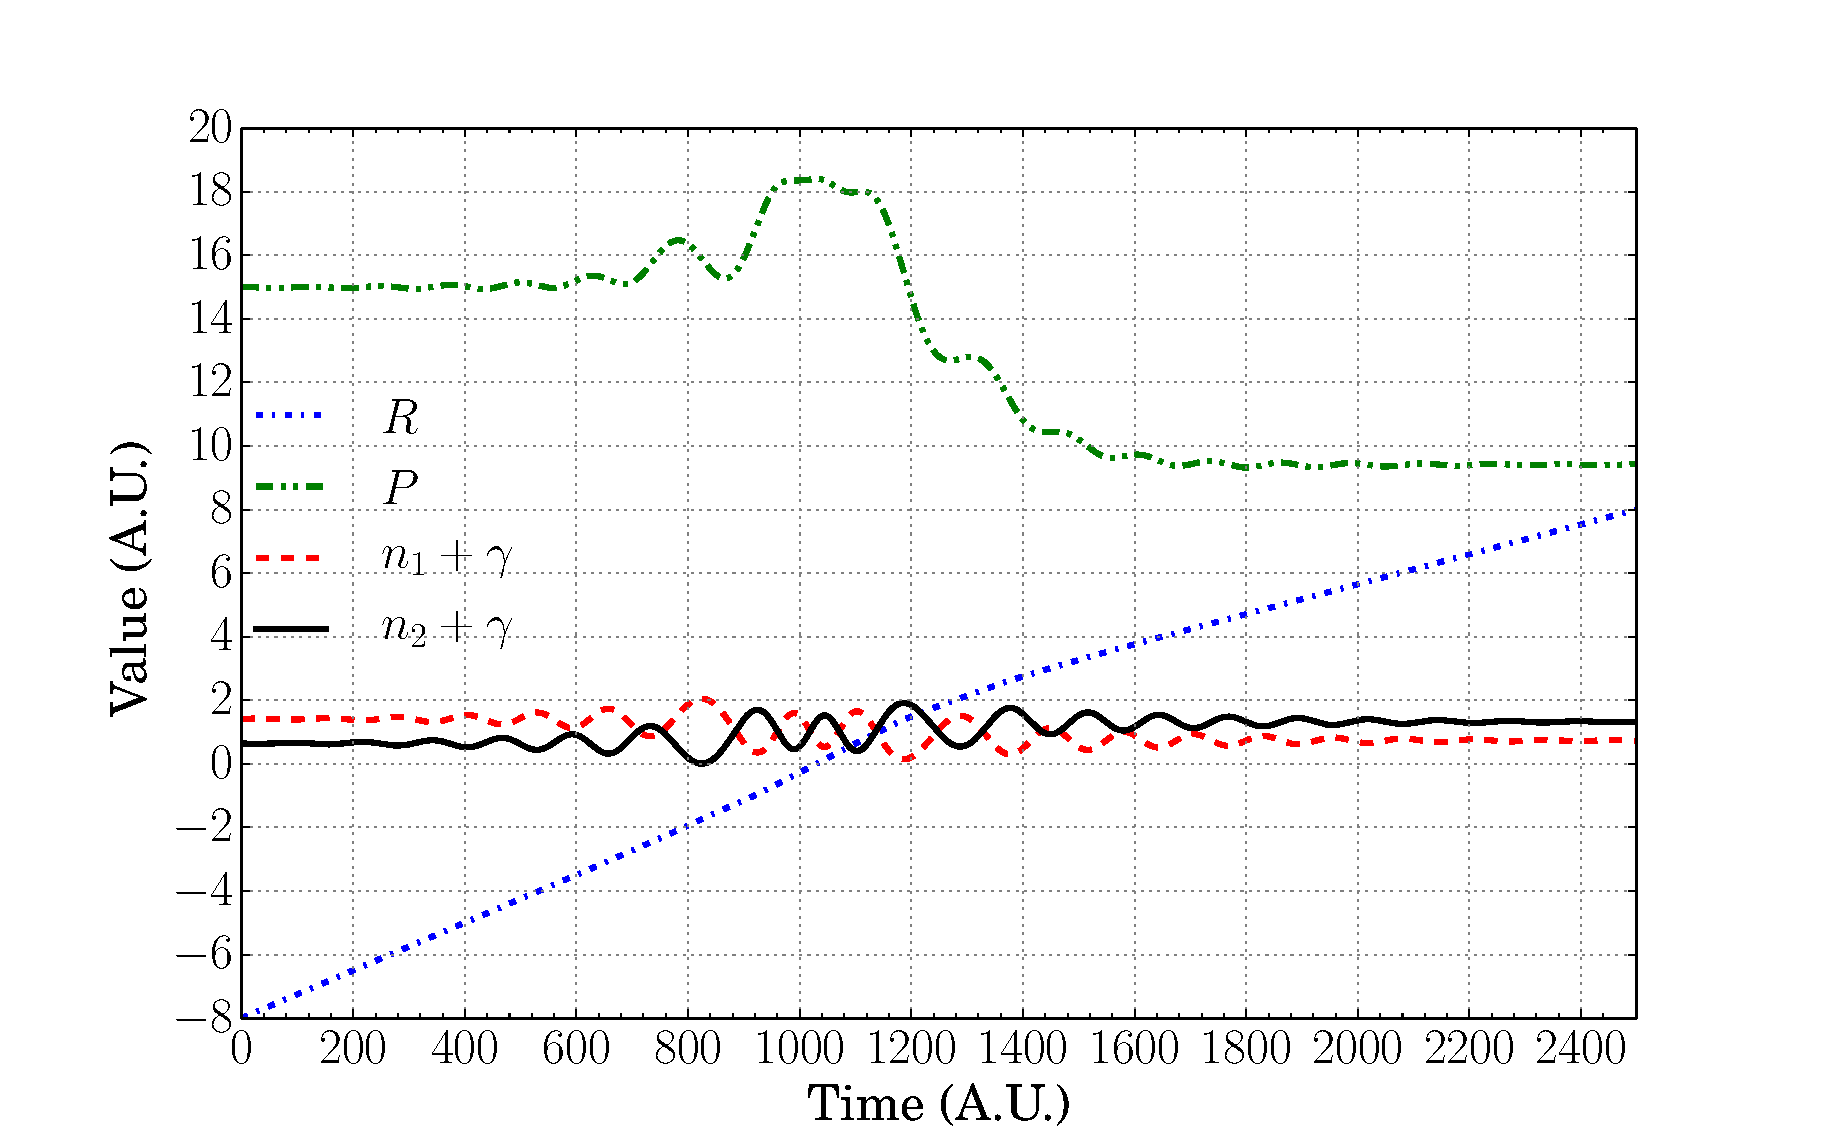
\includegraphics[width=\textwidth]{dc_traj_t21.eps}
\vspace{-0.1cm}
\caption{{\fontsize{7}{8}\selectfont \tto.}}
\end{subfigure}
~
\begin{subfigure}[t]{0.45\textwidth}
\centering
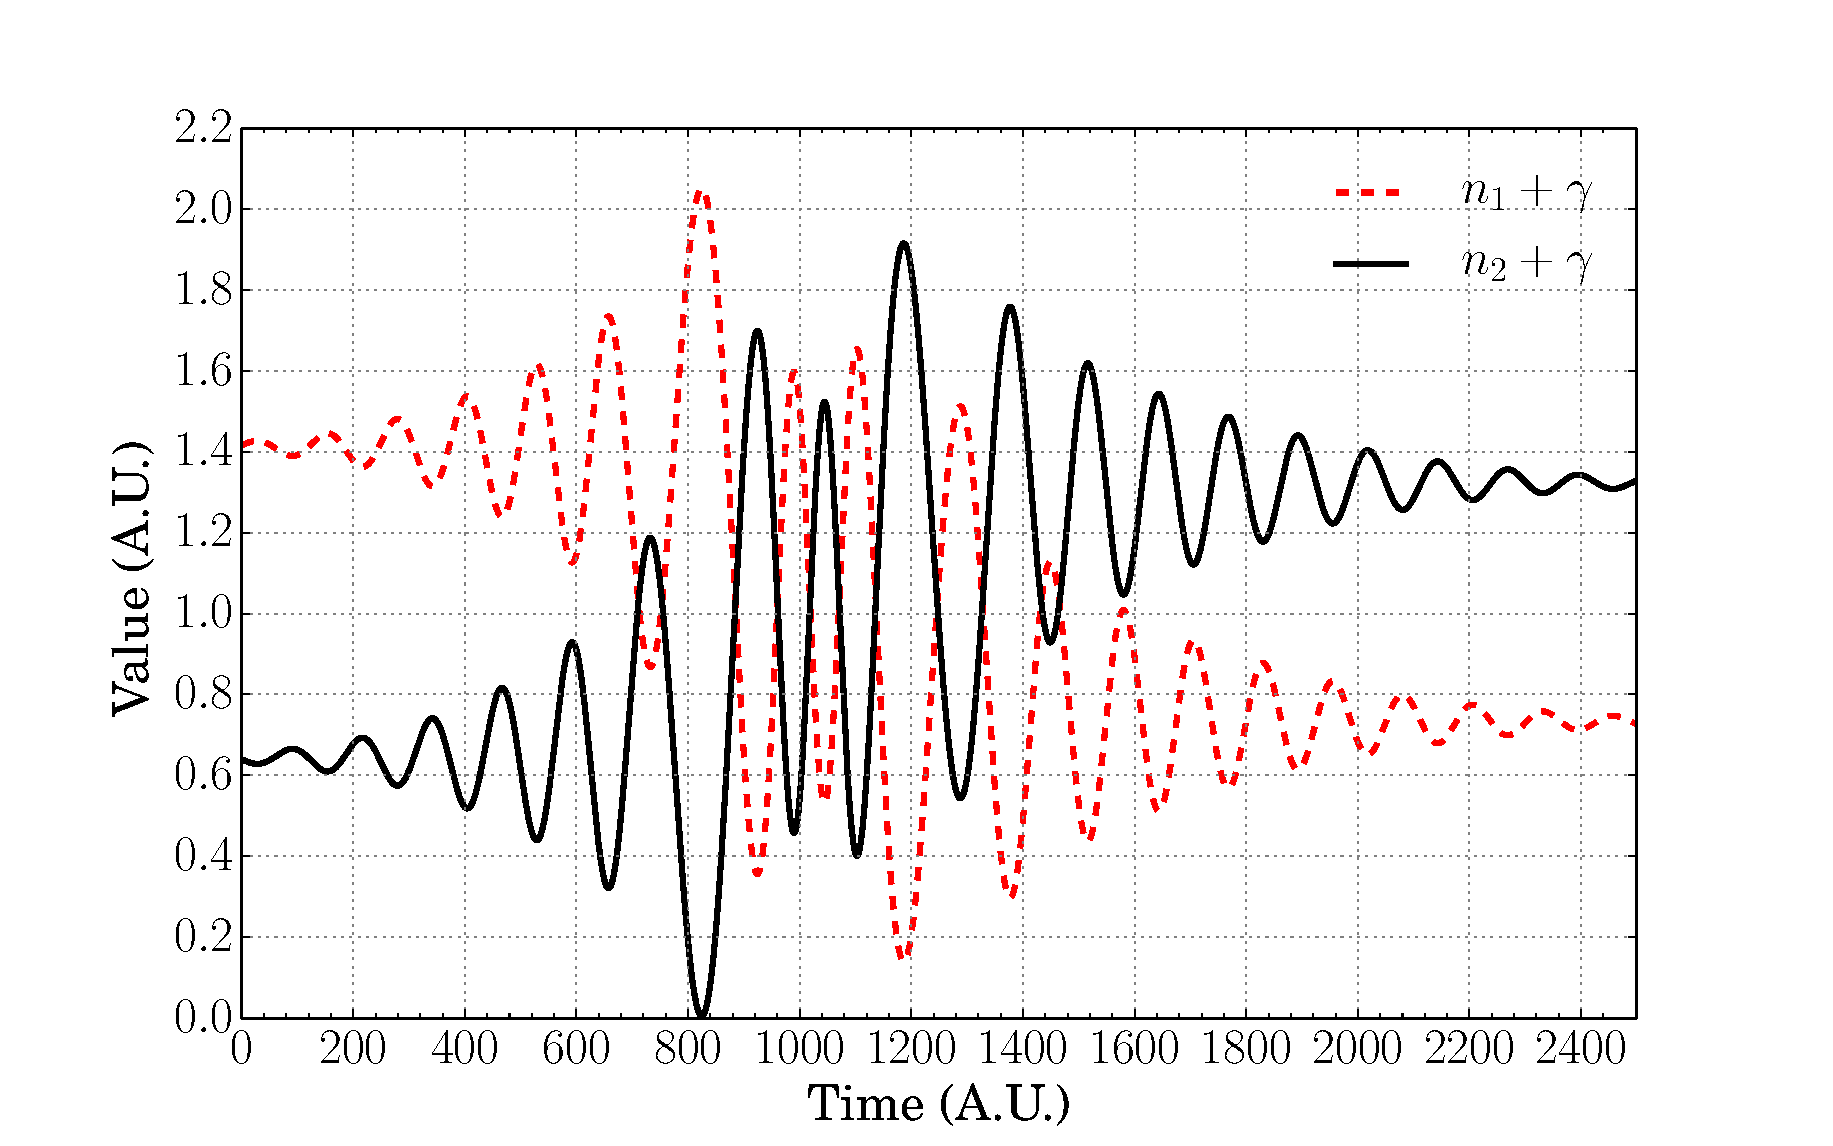
\includegraphics[width=\textwidth]{dc_traj_t21_e.eps}
\vspace{-0.1cm}
\caption{{\fontsize{7}{8}\selectfont \tto, zoom into $ n_{1}$, $n_{2} $.}}
\end{subfigure}
\vspace{-0.1cm}
\caption{$ i = 1 $, sample trajectories.}
\end{figure}
}{\stepcounter{figure}}

\alt<4>{
\framesubtitle{Sample Trajectories ($ i=1 $).}
\begin{figure}
\begin{subfigure}[t]{0.48\textwidth}
\centering
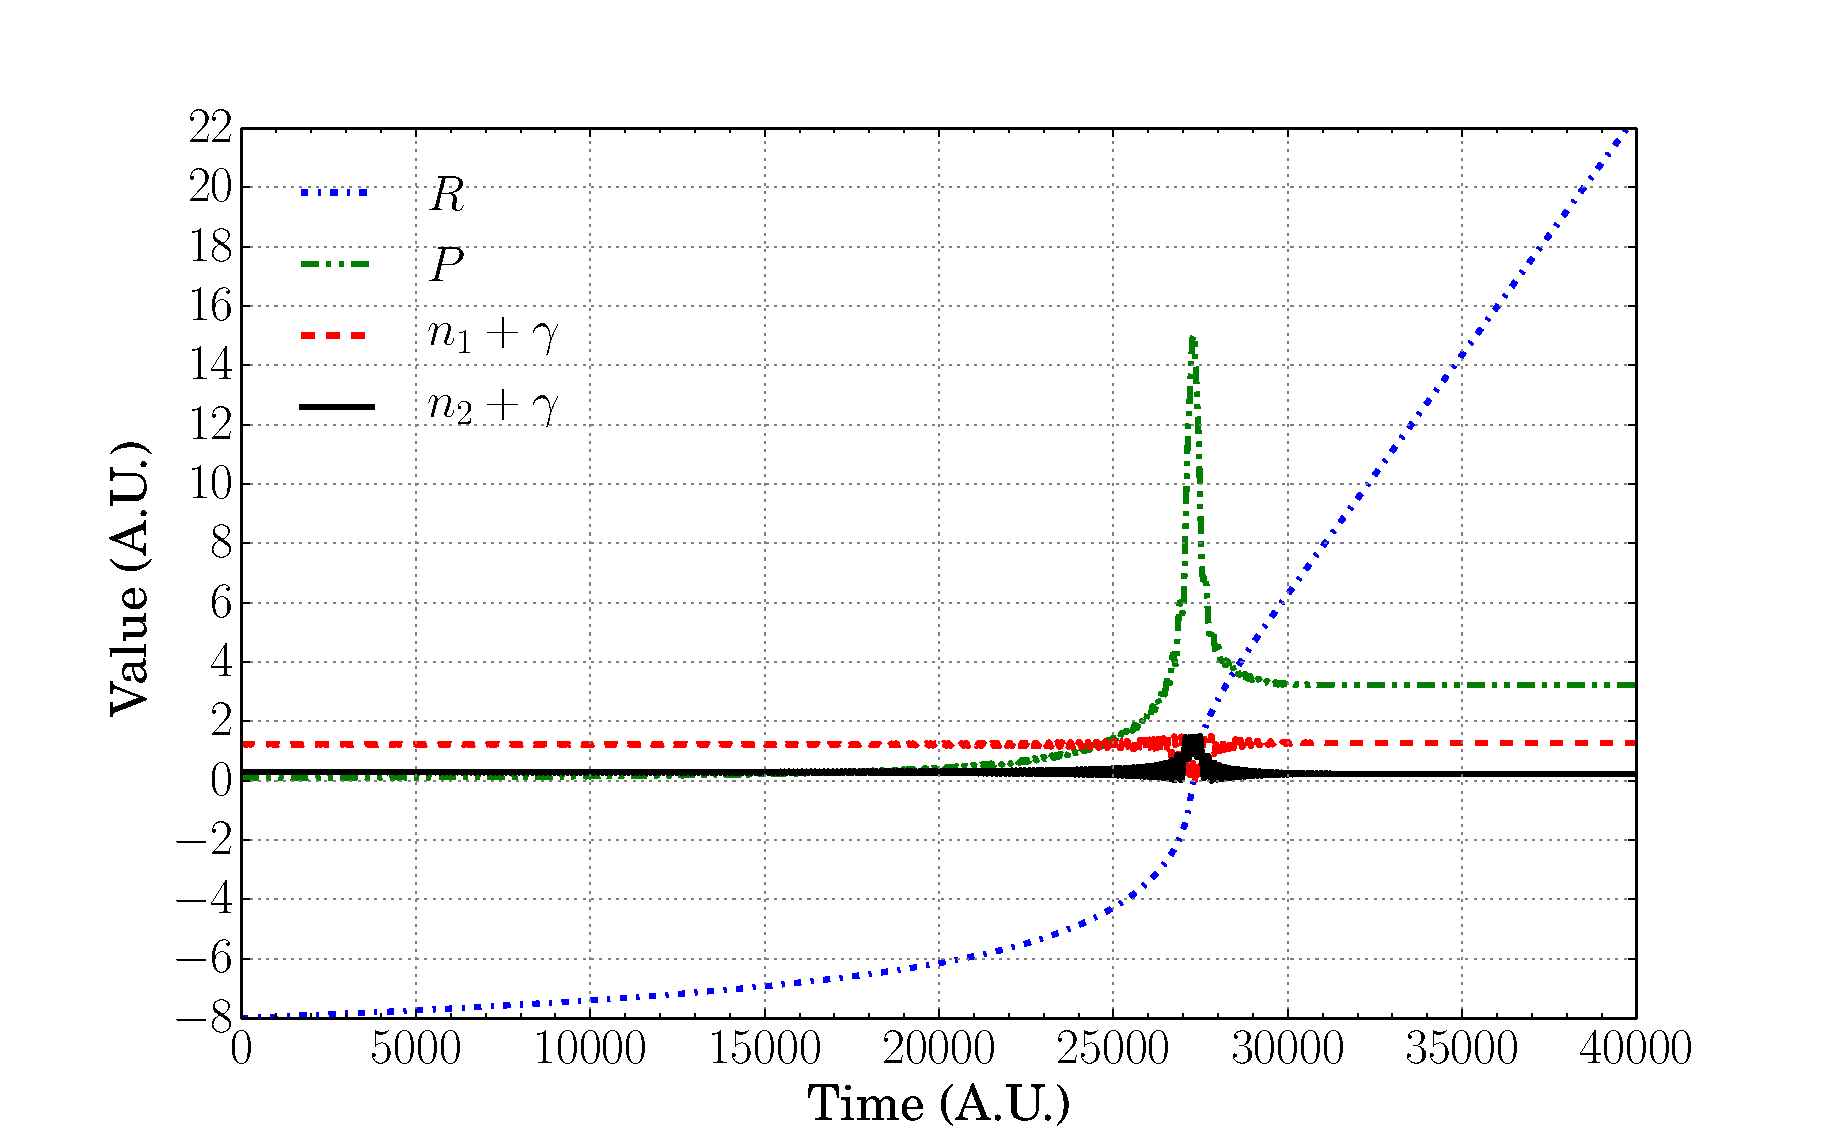
\includegraphics[width=\textwidth]{dc_traj_low_momentum.eps}
\caption{Low nuclear momentum.}
\end{subfigure}
~
\begin{subfigure}[t]{0.48\textwidth}
\centering
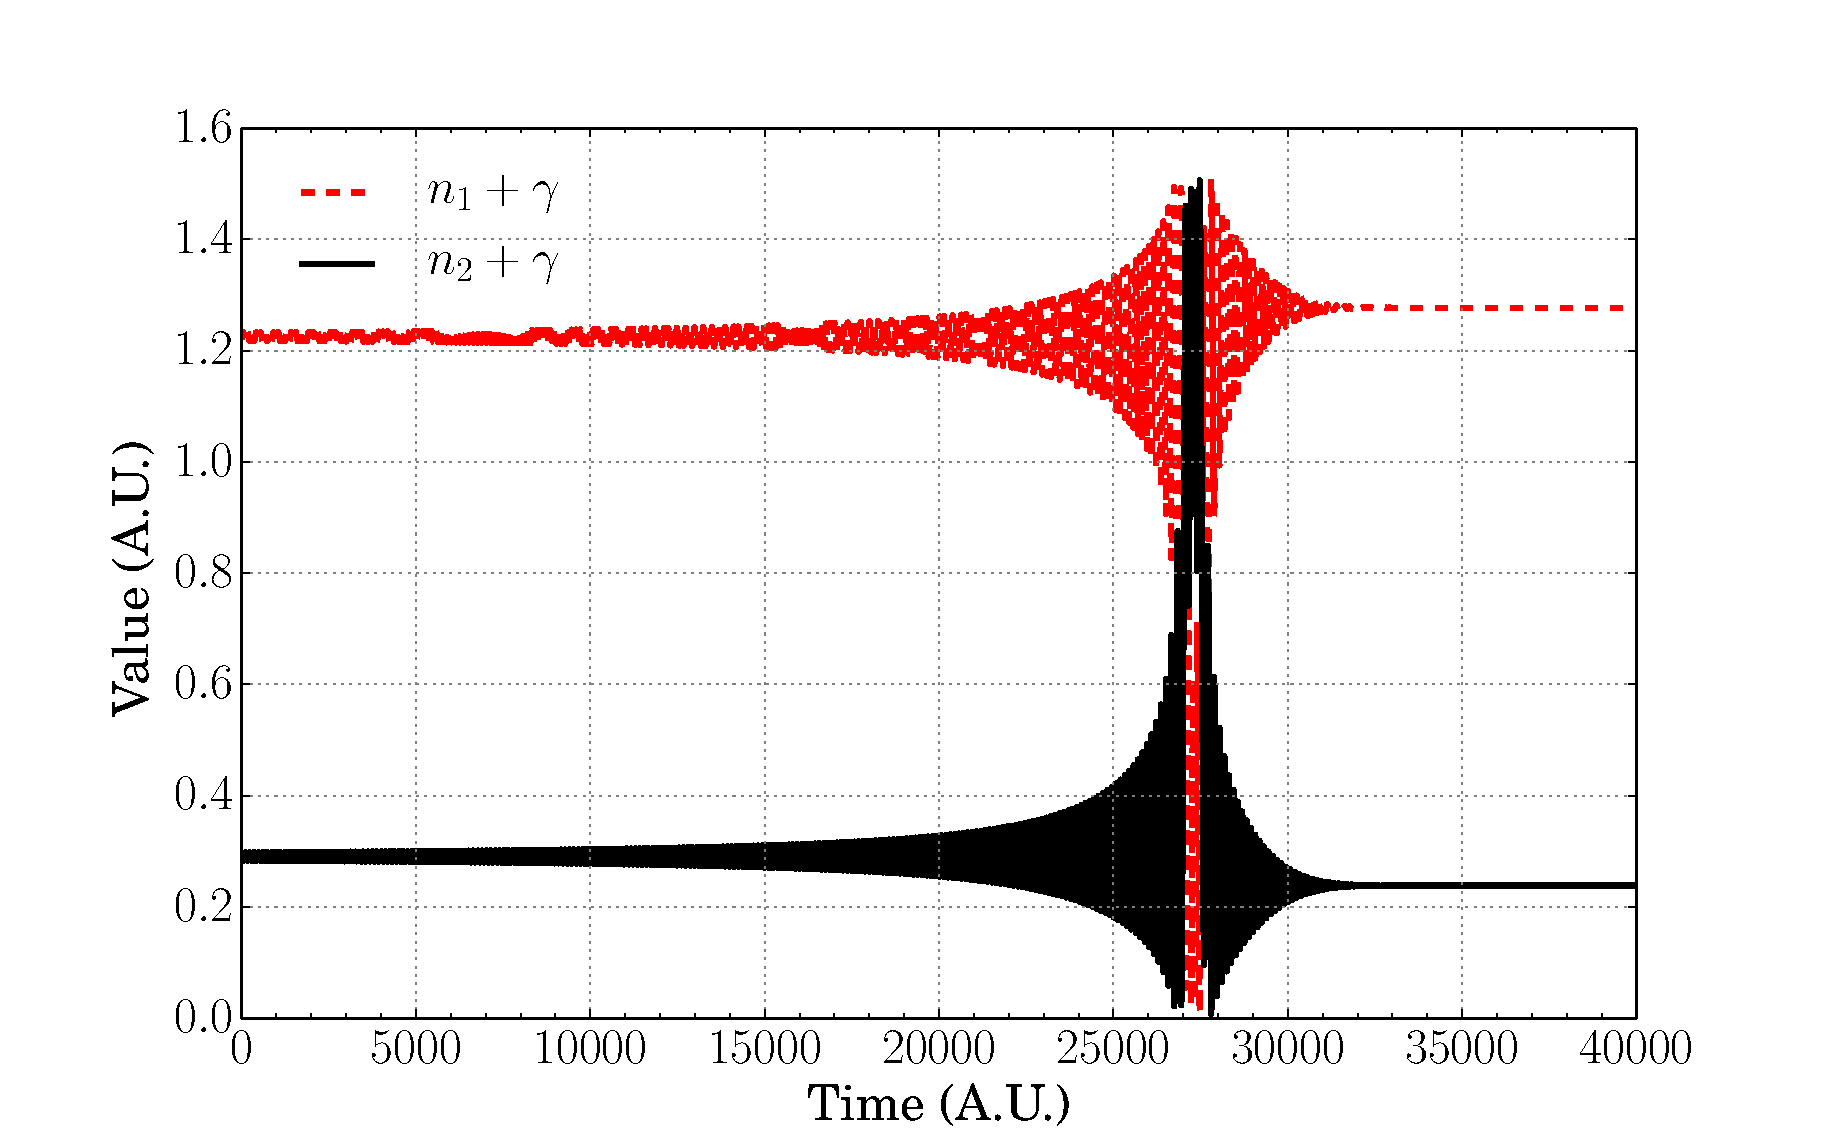
\includegraphics[width=\textwidth]{dc_traj_low_momentum_e.eps}
\caption{Low nuclear momentum, zoom into $ n_{1}$, $n_{2} $.}
\end{subfigure}
\caption{$ i = 1 $, trajectory examples.}
\end{figure}
}{\stepcounter{figure}}

\alt<5>{
\framesubtitle{Sample Trajectories ($ i=2 $).}
\vspace{-0.3cm}
\begin{figure}
\begin{subfigure}[t]{0.45\textwidth}
\centering
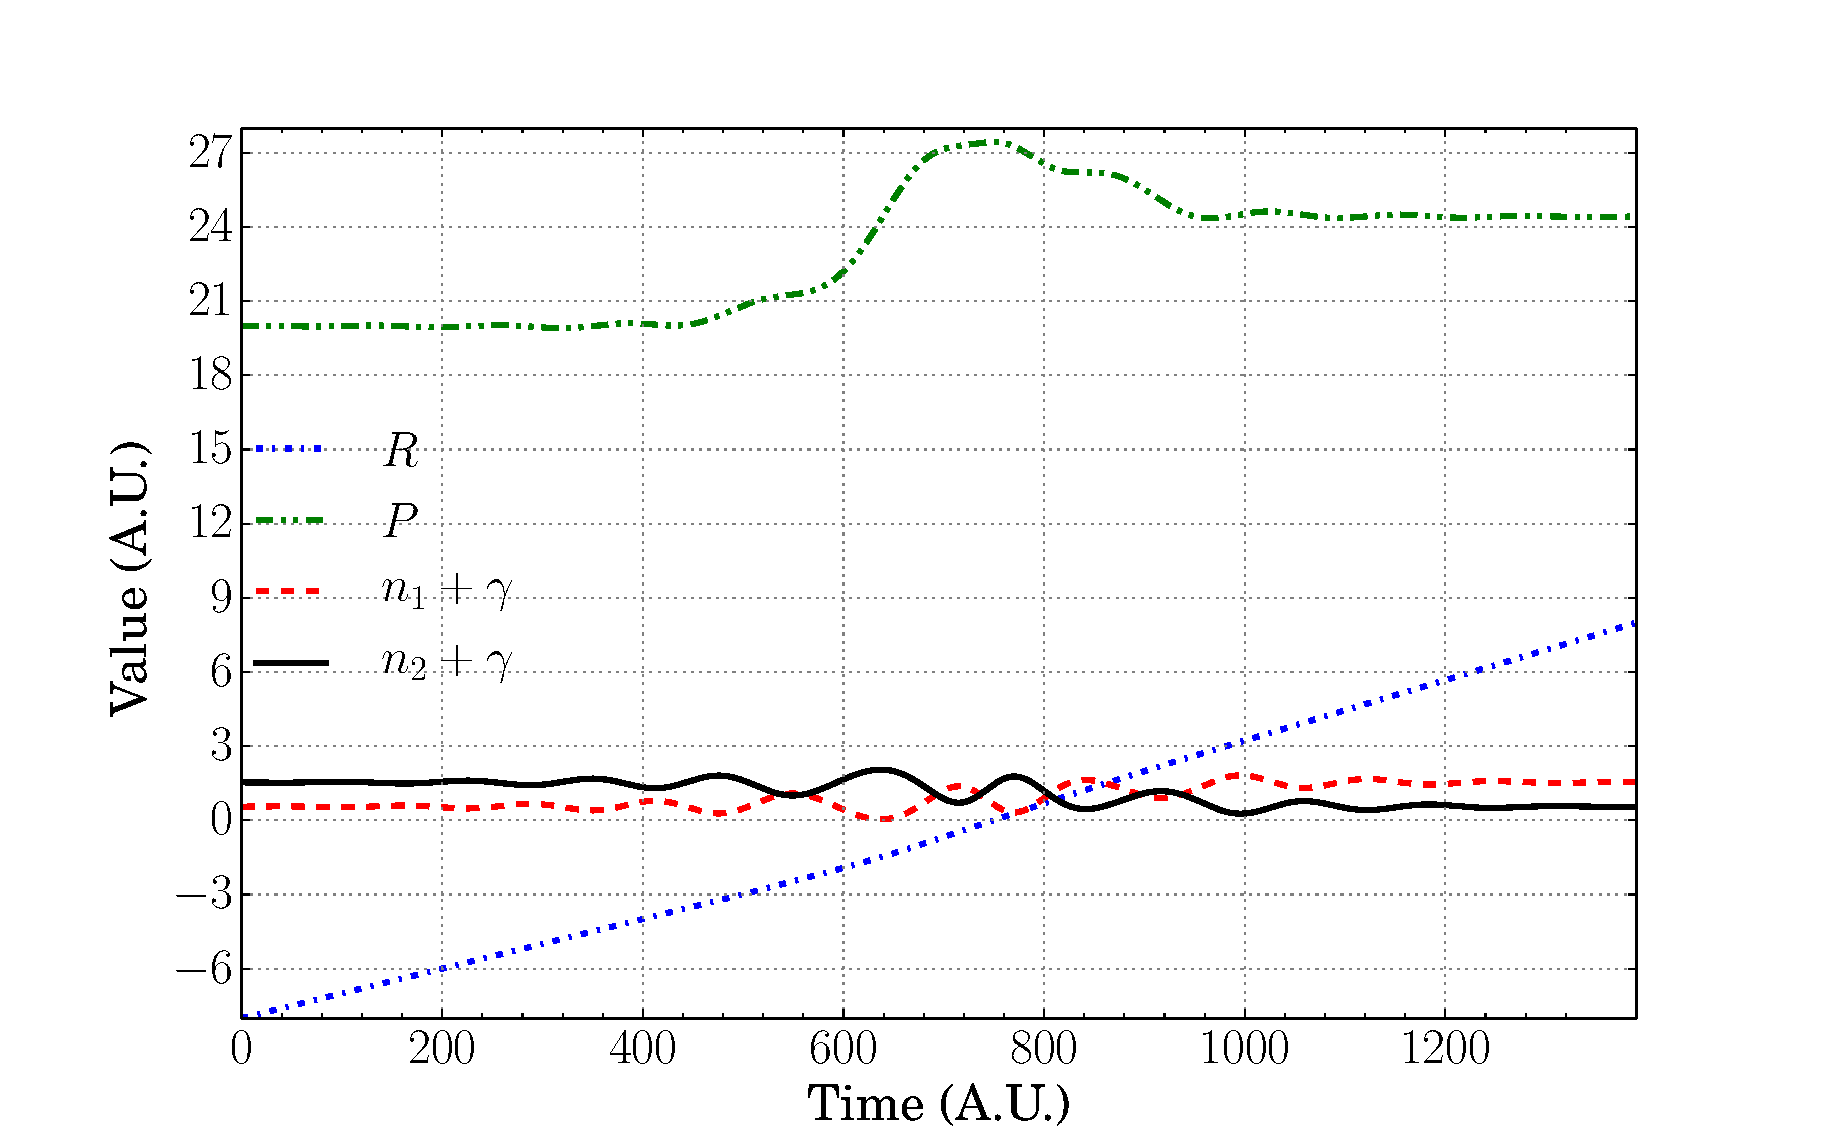
\includegraphics[width=\textwidth]{dc_traj_t12.eps}
\vspace{-0.1cm}
\caption{{\fontsize{7}{8}\selectfont \tot.}}
\end{subfigure}
~
\begin{subfigure}[t]{0.45\textwidth}
\centering
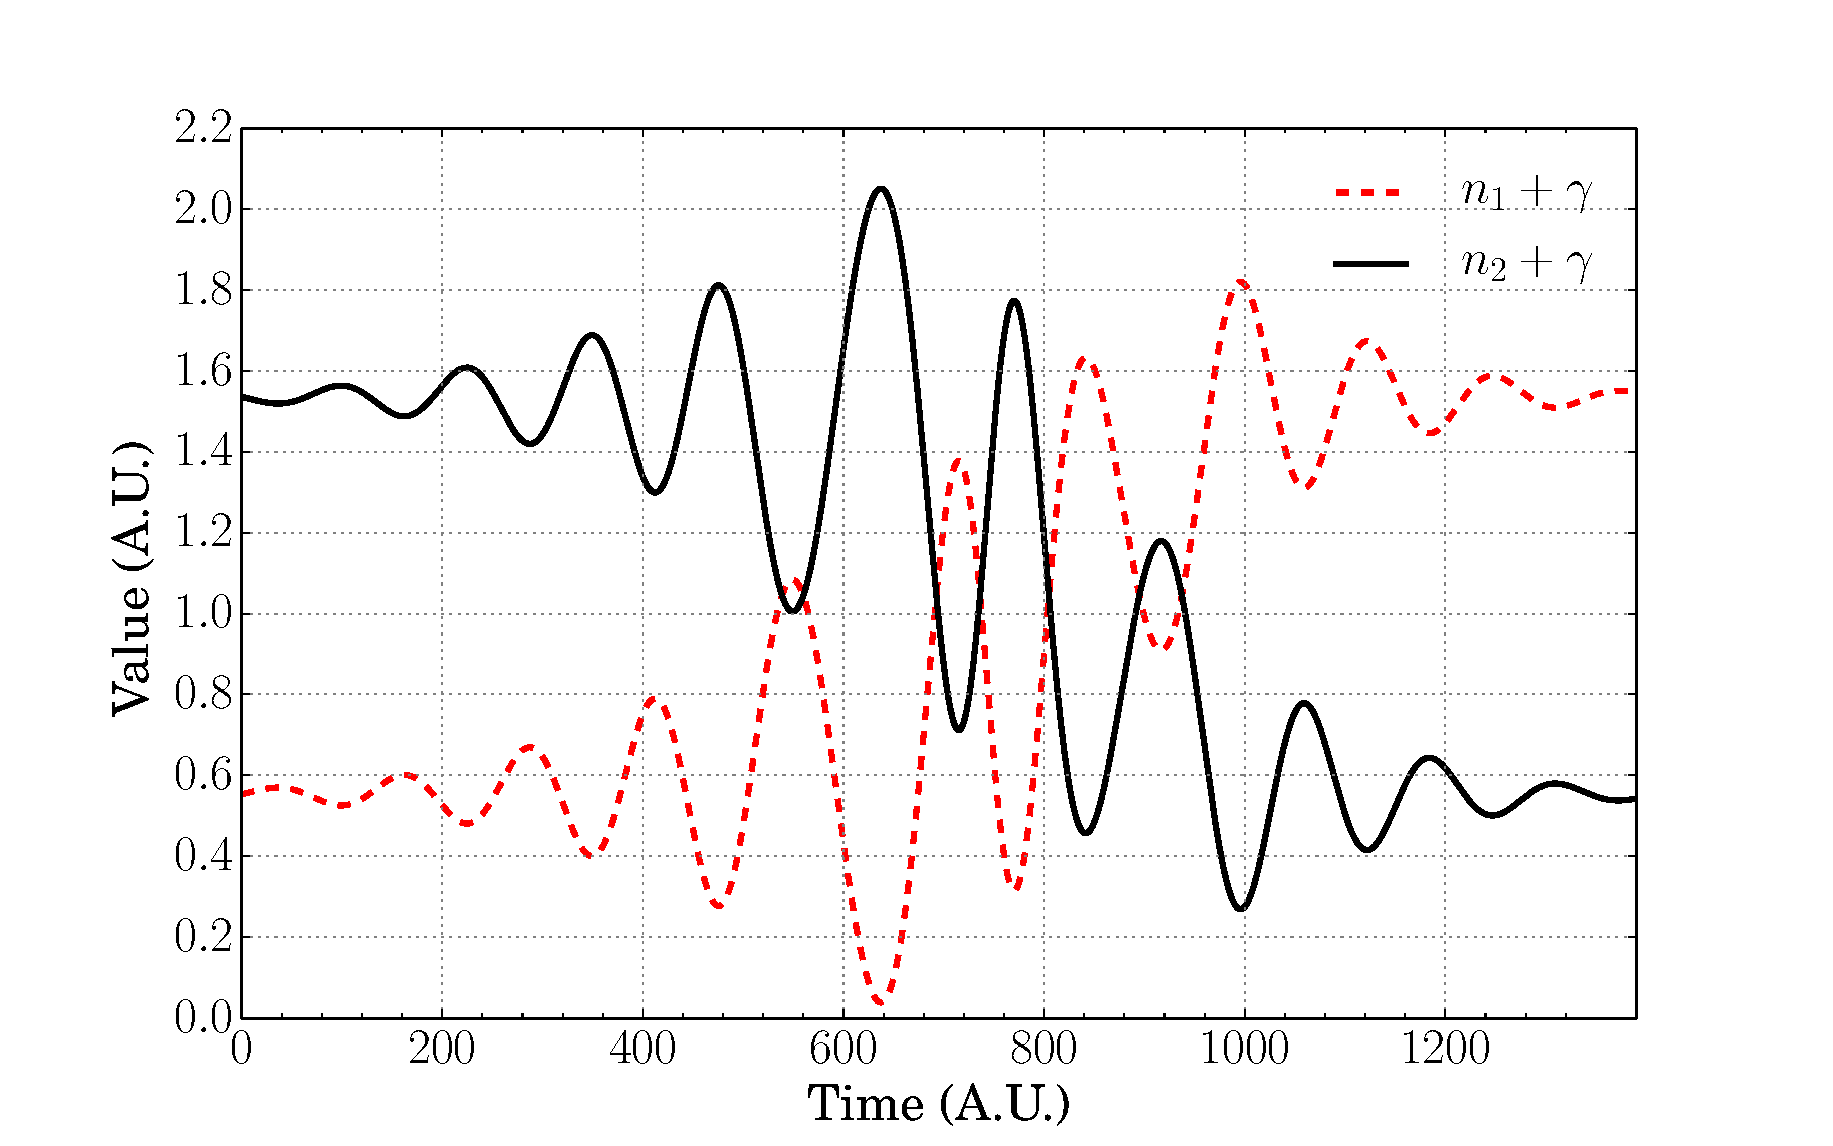
\includegraphics[width=\textwidth]{dc_traj_t12_e.eps}
\vspace{-0.1cm}
\caption{{\fontsize{7}{8}\selectfont \tot, zoom into $ n_{1} $, $ n_{2} $.}}
\end{subfigure}
\\[-0.32cm]
\begin{subfigure}[t]{0.45\textwidth}
\centering
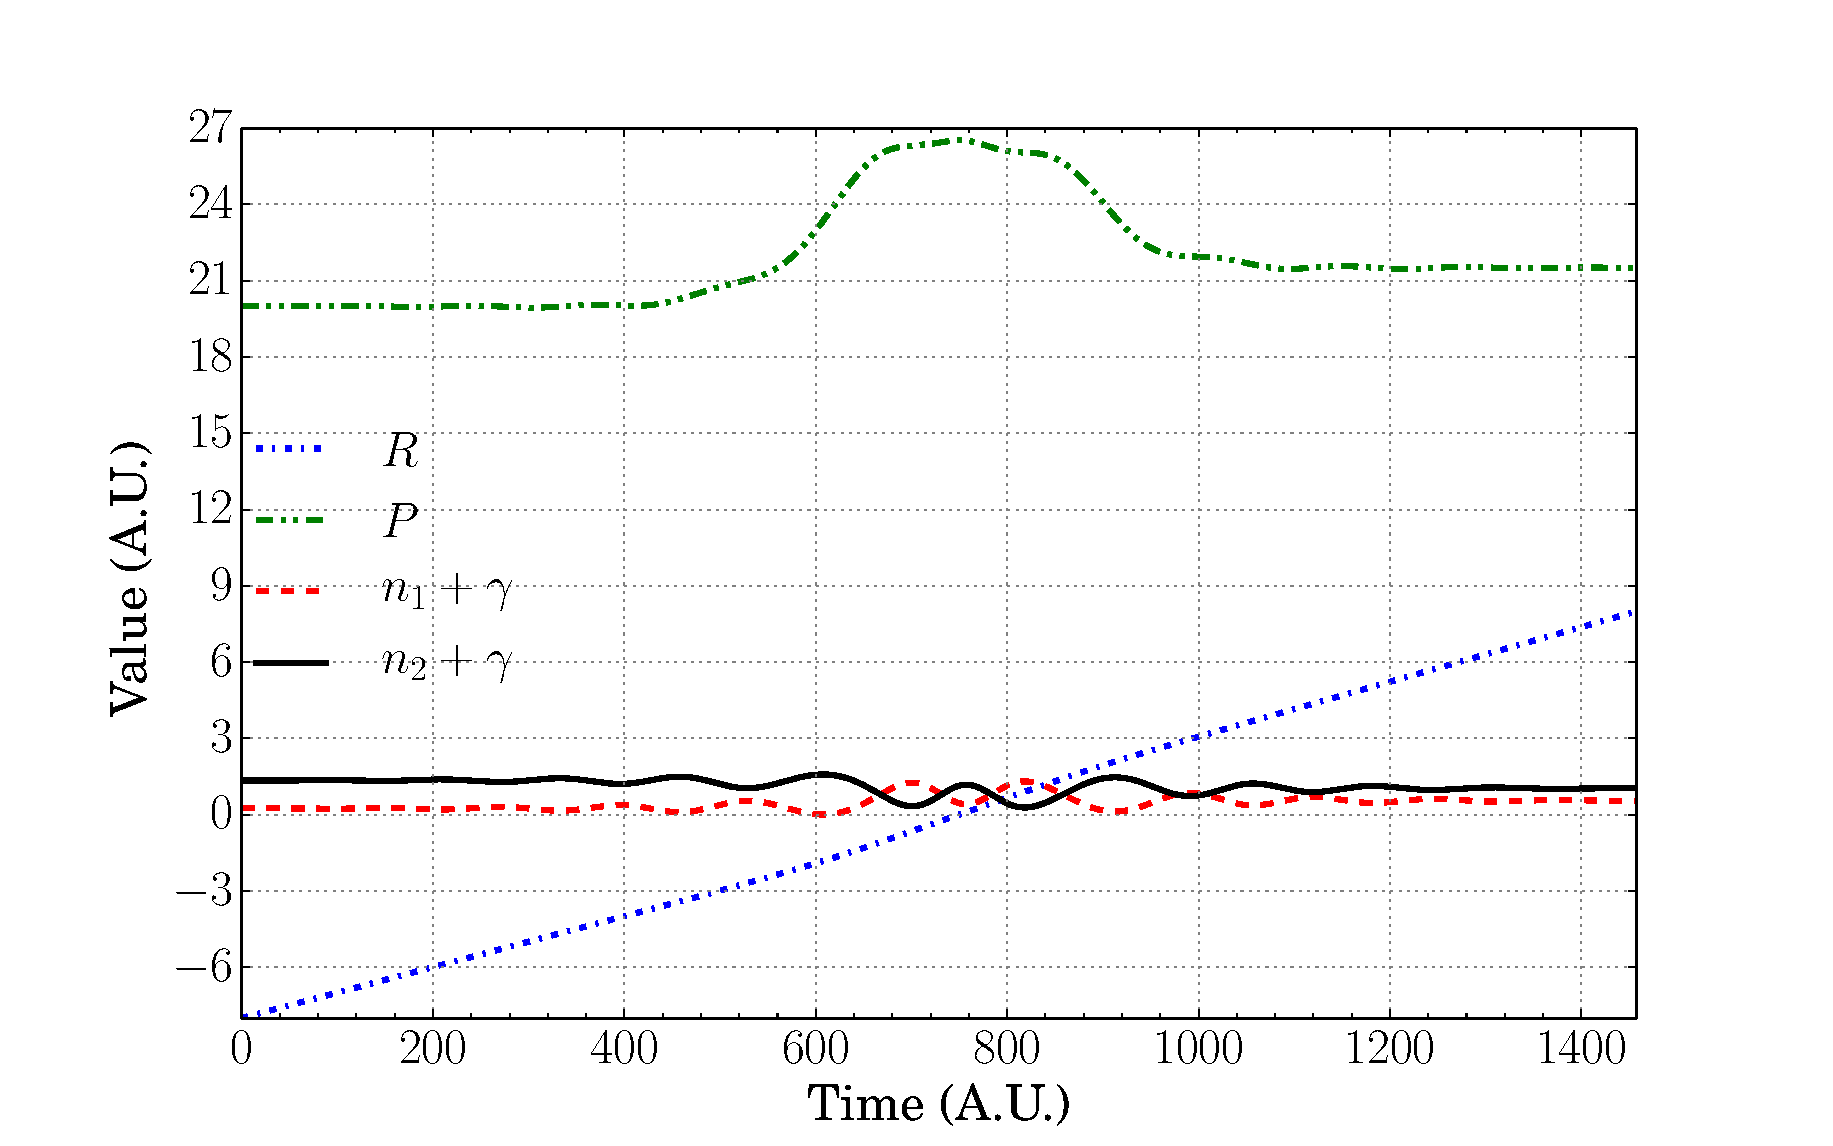
\includegraphics[width=\textwidth]{dc_traj_t22.eps}
\vspace{-0.1cm}
\caption{{\fontsize{7}{8}\selectfont \ttt.}}
\end{subfigure}
~
\begin{subfigure}[t]{0.45\textwidth}
\centering
\includegraphics[width=\textwidth]{dc_traj_t22_e.eps}
\vspace{-0.1cm}
\caption{{\fontsize{7}{8}\selectfont \ttt, zoom into $ n_{1}$, $n_{2} $.}}
\end{subfigure}
\caption{$ i = 2 $, trajectory examples.}
\end{figure}
}{\stepcounter{figure}}

\alt<6>{
\framesubtitle{Sample Trajectories ($ i=2 $).}
\begin{figure}
\begin{subfigure}[t]{0.48\textwidth}
\centering
\includegraphics[width=\textwidth]{dc_traj_low_momentum_2.eps}
\caption{Low nuclear momentum.}
\end{subfigure}
~
\begin{subfigure}[t]{0.48\textwidth}
\centering
\includegraphics[width=\textwidth]{dc_traj_low_momentum_e_2.eps}
\caption{Low nuclear momentum, zoom into $ n_{1}$, $n_{2} $.}
\end{subfigure}
\caption{$ i = 2 $, trajectory examples.}
\end{figure}
}{\stepcounter{figure}}
\end{frame}

\subsection{Extended Coupling}
\begin{frame}
\frametitle{Extended Coupling}
\alt<1>{
\framesubtitle{Diabatic PES Derivatives (DPES)}
\begin{subequations}
\begin{align}
\dpar{H_{11}}{R} &= \dpar{H_{22}}{R} = 0\\
\dpar{H_{12}}{R} &= \dpar{H_{21}}{R} = 
\begin{cases}
B C e^{-C R} &\mbox{if } R\geq 0\\
B C e^{C R} &\mbox{if } R<0
\end{cases}
\end{align}
\end{subequations}
}{\stepcounter{equation}}

\alt<2>{
\framesubtitle{Adiabatic PES (APES)}
\begin{subequations}
\begin{align}
E_{1} & = -
\sqrt{
A^{2} + 
\begin{cases}
B^{2} (2 - e^{-C R})^{2} &\mbox{if } R\geq 0\\
B^{2} e^{2 C R} &\mbox{if } R<0
\end{cases}
}\\
E_{2} &= -E_{1}
\end{align}
\end{subequations}
}{\stepcounter{equation}}

\alt<3>{
\framesubtitle{Derivatives of the APES (DAPES)}
\begin{subequations}
\begin{align}
\dpar{E_{1}}{R} &= 
\begin{cases}
-\frac{B^2 C e^{-2 C R} \left(2 e^{C R}-1\right)}{\sqrt{A^2+B^2 \left(e^{-C 
R}-2\right)^2}} & \mbox{if } R\geq 0\\
-\frac{B^2 C e^{2 C R}}{\sqrt{A^2+B^2 e^{2 C R}}} &\mbox{if } R<0
\end{cases}\\
\dpar{E_{2}}{R} &= -\dpar{E_{1}}{R}
\end{align}
\end{subequations}
}{\stepcounter{equation}}

\alt<4>{
\framesubtitle{Sample Trajectories ($ i=1 $).}
\vspace{-0.3cm}
\begin{figure}
\centering
\begin{subfigure}[t]{0.45\textwidth}
\centering
\includegraphics[width=\textwidth]{ec_traj_r11.eps}
\vspace{-0.1cm}
\caption{{\fontsize{7}{8}\selectfont \roo.}}
\end{subfigure}
~
\begin{subfigure}[t]{0.45\textwidth}
\centering
\includegraphics[width=\textwidth]{ec_traj_r11_e.eps}
\vspace{-0.1cm}
\caption{{\fontsize{7}{8}\selectfont \roo, zoom into $ n_{1}$, $n_{2} $.}}
\end{subfigure}
\\[-0.32cm]
\begin{subfigure}[t]{0.45\textwidth}
\centering
\includegraphics[width=\textwidth]{ec_traj_r21.eps}
\vspace{-0.1cm}
\caption{{\fontsize{7}{8}\selectfont \rto.}}
\end{subfigure}
~
\begin{subfigure}[t]{0.45\textwidth}
\centering
\includegraphics[width=\textwidth]{ec_traj_r21_e.eps}
\vspace{-0.1cm}
\caption{{\fontsize{7}{8}\selectfont \rto, zoom into $ n_{1}$, $n_{2} $.}}
\end{subfigure}
\vspace{-0.1cm}
\caption{$ i = 1 $, sample trajectories.}
\end{figure}
}{\stepcounter{figure}}

\alt<5>{
\framesubtitle{Sample Trajectories ($ i=1 $).}
\vspace{-0.3cm}
\begin{figure}
\centering
\begin{subfigure}[t]{0.45\textwidth}
\centering
\includegraphics[width=\textwidth]{ec_traj_t11.eps}
\vspace{-0.1cm}
\caption{{\fontsize{7}{8}\selectfont \too.}}
\end{subfigure}
~
\begin{subfigure}[t]{0.45\textwidth}
\centering
\includegraphics[width=\textwidth]{ec_traj_t11_e.eps}
\vspace{-0.1cm}
\caption{{\fontsize{7}{8}\selectfont \too, zoom into $ n_{1}$, $n_{2} $.}}
\end{subfigure}
\\[-0.32cm]
\begin{subfigure}[t]{0.45\textwidth}
\centering
\includegraphics[width=\textwidth]{ec_traj_t21.eps}
\vspace{-0.1cm}
\caption{{\fontsize{7}{8}\selectfont \tto.}}
\end{subfigure}
~
\begin{subfigure}[t]{0.45\textwidth}
\centering
\includegraphics[width=\textwidth]{ec_traj_t21_e.eps}
\vspace{-0.1cm}
\caption{{\fontsize{7}{8}\selectfont \tto, zoom into $ n_{1}$, $n_{2} $.}}
\end{subfigure}
\vspace{-0.1cm}
\caption{$ i = 1 $, sample trajectories.}
\end{figure}
}{\stepcounter{figure}}

\alt<6>{
\framesubtitle{Sample Trajectories ($ i=2 $).}
\vspace{-0.3cm}
\begin{figure}
\centering
\begin{subfigure}[t]{0.45\textwidth}
\centering
\includegraphics[width=\textwidth]{ec_traj_r12.eps}
\vspace{-0.1cm}
\caption{{\fontsize{7}{8}\selectfont \rot.}}
\end{subfigure}
~
\begin{subfigure}[t]{0.45\textwidth}
\centering
\includegraphics[width=\textwidth]{ec_traj_r12_e.eps}
\vspace{-0.1cm}
\caption{{\fontsize{7}{8}\selectfont \rot, zoom into $ n_{1}$, $n_{2} $.}}
\end{subfigure}
\\[-0.32cm]
\begin{subfigure}[t]{0.45\textwidth}
\centering
\includegraphics[width=\textwidth]{ec_traj_r22.eps}
\vspace{-0.1cm}
\caption{{\fontsize{7}{8}\selectfont \rtt.}}
\end{subfigure}
~
\begin{subfigure}[t]{0.45\textwidth}
\centering
\includegraphics[width=\textwidth]{ec_traj_r22_e.eps}
\vspace{-0.1cm}
\caption{{\fontsize{7}{8}\selectfont \rtt, zoom into $ n_{1}$, $n_{2} $.}}
\end{subfigure}
\vspace{-0.1cm}
\caption{$ i = 2 $, sample trajectories.}
\end{figure}
}{\stepcounter{figure}}

\alt<7>{
\framesubtitle{Sample Trajectories ($ i=2 $).}
\vspace{-0.3cm}
\begin{figure}
\centering
\begin{subfigure}[t]{0.45\textwidth}
\centering
\includegraphics[width=\textwidth]{ec_traj_t21.eps}
\vspace{-0.1cm}
\caption{{\fontsize{7}{8}\selectfont \tto.}}
\end{subfigure}
~
\begin{subfigure}[t]{0.45\textwidth}
\centering
\includegraphics[width=\textwidth]{ec_traj_t21_e.eps}
\vspace{-0.1cm}
\caption{{\fontsize{7}{8}\selectfont \tto, zoom into $ n_{1}$, $n_{2} $.}}
\end{subfigure}
\\[-0.32cm]
\begin{subfigure}[t]{0.45\textwidth}
\centering
\includegraphics[width=\textwidth]{ec_traj_t22.eps}
\vspace{-0.1cm}
\caption{{\fontsize{7}{8}\selectfont \ttt.}}
\end{subfigure}
~
\begin{subfigure}[t]{0.45\textwidth}
\centering
\includegraphics[width=\textwidth]{ec_traj_t22_e.eps}
\vspace{-0.1cm}
\caption{{\fontsize{7}{8}\selectfont \ttt, zoom into $ n_{1}$, $n_{2} $.}}
\end{subfigure}
\vspace{-0.1cm}
\caption{$ i = 2 $, sample trajectories.}
\end{figure}
}{\stepcounter{figure}}
\end{frame}

\subsection{Condensed-Phase Spin-Boson Model}
\begin{frame}
\frametitle{Condensed-Phase Spin-Boson Model}
\alt<1>{
\framesubtitle{Diabatic PES Derivatives (DPES)}
\begin{subequations}
\begin{align}
\dpar{H_{11}}{\bm{Q}} &= \sum\limits_{k=1}^{M} m_{k} \omega_{k}^{2} Q_{k} + \sum\limits_{k=1}^{M} c_{k}\\
\dpar{H_{22}}{\bm{Q}} &= \sum\limits_{k=1}^{M} m_{k} \omega_{k}^{2} Q_{k} - \sum\limits_{k=1}^{M} c_{k}\\
\dpar{H_{12}}{\bm{Q}} &= \dpar{H_{21}}{\bm{Q}} = 0
\end{align}
\end{subequations}
}{\stepcounter{equation}}

\alt<2>{
\framesubtitle{Nuclear Equations of Motion}
\begin{itemize}
\item There are $ M $ nuclear degrees of freedom (DOFs) and $ F $ electronic degrees of freedom $ \therefore $ there are $ 2 M + 2 F $ equations of motion.
\item In our case, $ F = 2 $ so the nuclear equations of motion are:
\end{itemize}
\begin{subequations}
\begin{align}
\dot{Q}_{j} & = \frac{P_{j}}{m_{j}}\\
\dot{P}_{j} & = -m_{j}\omega_{j}^{2}Q_{j} - \frac{1}{2} c_{j}(p_{1}^{2} + x_{1}^{2} - p_{2}^{2} - x_{2}^{2})
\end{align}
\end{subequations}
\begin{itemize}
\item They were implemented with a loop.
\end{itemize}
}{\stepcounter{equation}}

\alt<3>{
\framesubtitle{Frequencies}
\begin{itemize}
\item It was assumed that $ \omega_{k} $ are uniformly distributed $ \in [0.01 \omega_{c},~4 \omega_{c}] $ \textcolor{blue}{\cite{spin-boson}}, where $ \omega_{c} $ is the `characteristic frequency'.
\item Frequencies contribute to the system's energy differently so each has a coupling parameter $ c_{k} $.
\end{itemize}
\begin{subequations}
\begin{align}
J(\omega) &= \frac{\pi}{2} \sum\limits_{k=1}^{M} \frac{c_{k}^{2}}{m_{k} \omega_{k}}  \delta(\omega - \omega_{k})\\
J(\omega) &= \frac{\pi}{2} \alpha \omega \exp\left(-\frac{\omega}{\omega_{c}}\right)
\end{align}
\end{subequations}
\begin{itemize}
\item Where $ \alpha \equiv $ Kondo parameter (coupling strength).
\end{itemize}
}{\stepcounter{equation}}

\alt<4>{
\framesubtitle{Frequencies}
\begin{itemize}
\item Upon integrating with respect to $ \omega $, the coupling parameters can be calculated as:
\end{itemize}
\begin{subequations}
\begin{align}
c_{k} &= \omega_{k} \sqrt{\alpha \Delta \omega m_{k} \exp\left(-\frac{\omega_{k}}{\omega_{c}}\right)} \\
\Delta \omega &= \frac{\omega_{max} - \omega_{min}}{M - 1}
\end{align}
\end{subequations}
}{\stepcounter{equation}}

\alt<5>{
\framesubtitle{Initial Conditions}
\begin{itemize}
\item There is no covariant element $ \therefore $ nuclear momenta and positions can be independently sampled from gaussian distributions.
\item The standard deviation ($ \sigma $) and mean values ($ \mu $) for each of them are:
\end{itemize}
\begin{subequations}
\begin{align}
&\sigma_{P_{k}} = \sqrt{\frac{m_{k} \omega_{k}}{2 \tanh\left(\frac{\beta \omega_{k}}{2}\right)}}~~&&,~~
&&\mu_{P_{k}} = 0\\
&\sigma_{Q_{k}} = \sqrt{\frac{1}{2 m_{k} \omega_{k} \tanh\left(\frac{\beta \omega_{k}}{2}\right)}}~~&&,~~
&&\mu_{Q_{k}} = -\frac{c_{k}}{m_{k} \omega_{k}^{2}}
\end{align}
\end{subequations}
}{\stepcounter{equation}}
\end{frame}

\subsection{Main Code}
\begin{frame}
\frametitle{Main Code}
\only<1>{
\begin{itemize}
\item Main program.
\begin{enumerate}
\item[1)] Call data collection subroutine.
\item[2)] Call print PES and DPES subroutine.
\end{enumerate}
\item Data collection subroutine.
\begin{enumerate}
\item[1)] Declare and initialise variables.
\item[2)] Open output file.
\item[3)] Write heading on file.
\item[4)] Define value of initial momentum.
\item[5)] Call Monte-Carlo averaging routine.
\item[6)] Write final results.
\begin{itemize}
\item Repeat 4) to 6) for other initial momentum values.
\end{itemize}
\end{enumerate}
\end{itemize}
}
\only<2>{
\begin{itemize}
\item Monte-Carlo averaging subroutine.
\begin{enumerate}
\item[1)] Declare and intialise variables.
\item[2)] Define Monte-Carlo steps loop.
\begin{enumerate}
\item[a)] Call solution subroutine.
\item[b)] Add results.
\end{enumerate}
\item[3)] Average results with the number of Monte-Carlo steps.
\item[4)] Calculate transition probabilities for reflection and transmission.
\end{enumerate}
\end{itemize}
}
\only<3>{
\begin{itemize}
\item Solution subroutine.
\begin{enumerate}
\item[1)] Declare and initialise variables.
\item[2)] Define and calculate initial conditions and window functions.
\item[3)] Define integration loop.
\begin{enumerate}
\item[a)] Call RK4G subroutine using the appropriate equations of motion as argument.
\item[b)] Check for reflection, exit loop if the particle was reflected.
\item[c)] Update the initial conditions for next integration step.
\end{enumerate}
\item[4)] Calculate final values for the acceptance criteria.
\item[5)] Calculate final window functions.
\item[6)] Calculate results for the Monte-Carlo averaging subroutine.
\end{enumerate}
\end{itemize}
}
\only<4>{
\begin{itemize}
\item Equations of motion subroutine.
\begin{enumerate}
\item[1)] Define and initialise variables.
\item[2)] Define equations of motion.
\end{enumerate}

\begin{itemize}
\item PES or DPES subroutines.
\begin{enumerate}
\item[1)] Define and initialise variables.
\item[2)] Check which PES or DPES are required.
\item[3)] Define PES or DPES.
\end{enumerate}
\end{itemize}
\end{itemize}
}
\only<5>{
\begin{itemize}
\item Runge-Kutta 4 Gill numerical integration routine (RK4G).
\begin{enumerate}
\item[1)] Define and initialise variables.
\item[2)] Call equations of motion subroutine.
\begin{itemize}
\item Calculate the intermediate step for all independent variables.
\end{itemize}
\item[3)] Repeat 2. for every intermediate step.
\item[4)] Calculate the final value of every independent variable, to be used in the next integration step.
\end{enumerate}
\end{itemize}
}
\only<6>{
\begin{itemize}
\item PES and DPES printing subroutine.
\begin{enumerate}
\item[1)] Define and initialise variables.
\item[2)] Define loop to print all functions.
\begin{enumerate}
\item[a)] Open relevant output file.
\item[b)] Call PES and DPES subroutines.
\item[c)] Write numerical values of each PES and DPES function, evaluated at any given distance.
\begin{itemize}
\item Repeat b) and c) for all desired distances.
\end{itemize}
\end{enumerate}
\end{enumerate}
\end{itemize}
}
\end{frame}
\end{document}